%%%%%%%%%%%%%%%%%%%%%%%%%%%%%%%%%%%%%%%%%
% Master Thesis - HPC Sorting Serious Game
% University of Genova
%
% Author: Szymon Zinkowicz
% Supervisor: Professor Daniele D'Agostino
% Reviewer: Professor Maura Cerioli
%
% License: MIT
%%%%%%%%%%%%%%%%%%%%%%%%%%%%%%%%%%%%%%%%%

\documentclass[twoside]{./class/masterthesis}

%-----------------------------------------------------------------------
%	PACKAGES
%-----------------------------------------------------------------------

\usepackage[utf8]{inputenc}
\usepackage[T1]{fontenc}
\usepackage{lmodern}
\usepackage[english]{babel}
\usepackage{csquotes}
\usepackage{graphicx}
\usepackage{amsmath,amssymb,amsthm}
\usepackage[table, dvipsnames]{xcolor}
\usepackage[backend=biber,style=ieee,sorting=none,natbib=true]{biblatex}
\usepackage{hyperref}
\usepackage{subcaption}
\usepackage{caption}
\usepackage{lipsum}
\usepackage{fancyhdr}
\usepackage{float}
\usepackage{siunitx}
\usepackage{booktabs}
\usepackage{array,multirow,makecell}
\usepackage{adjustbox}
\usepackage{listings}
\usepackage{geometry}
\usepackage{titlesec}
\usepackage{tocloft}
\usepackage{mdframed}
\usepackage{microtype}

%-----------------------------------------------------------------------
%	GEOMETRY
%-----------------------------------------------------------------------

\geometry{
	top=3cm,
	bottom=3cm,
	left=3.5cm,
	right=2.5cm,
	headheight=15pt
}

%-----------------------------------------------------------------------
%	HYPERREF SETUP
%-----------------------------------------------------------------------

\hypersetup{
	colorlinks=true,
	linktoc=all,
	linkcolor=blue,
	citecolor=blue,
	urlcolor=blue,
	pdfauthor={Szymon Zinkowicz},
	pdftitle={HPC Sorting Serious Game: A Web-First Educational Approach},
}

%-----------------------------------------------------------------------
%	CODE LISTING SETUP
%-----------------------------------------------------------------------
  
\definecolor{codegreen}{rgb}{0,0.6,0}
\definecolor{codegray}{rgb}{0.5,0.5,0.5}
\definecolor{codepurple}{rgb}{0.58,0,0.82}
\definecolor{backcolour}{rgb}{0.95,0.95,0.92}
 
\lstdefinestyle{gdscript}{
    numberstyle=\tiny\color{codegray},
    stringstyle=\color{codepurple},
    belowcaptionskip=1\baselineskip,
    frame=none,
    basicstyle=\footnotesize\ttfamily,
    keywordstyle=\bfseries\color{green!40!black},
    commentstyle=\itshape\color{purple!40!black},
    identifierstyle=\color{blue},
    backgroundcolor=\color{gray!10!white},
    breakatwhitespace=false,
    breaklines=true,
    captionpos=b,
    keepspaces=true,
    numbers=left,
    numbersep=5pt,
    showspaces=false,
    showstringspaces=false,
    showtabs=false,
    tabsize=4,
    language=Python, % GDScript is Python-like
    mathescape=false
}

\lstset{style=gdscript}

%-----------------------------------------------------------------------
%	BIBLIOGRAPHY
%-----------------------------------------------------------------------

\addbibresource{references.bib}

%-----------------------------------------------------------------------
%	CUSTOM MACROS
%-----------------------------------------------------------------------

% Convenient macros for frequently used terms
\newcommand*\openmp{OpenMP}
\newcommand*\mpi{MPI}
\newcommand*\gdscript{GDScript}
\newcommand*\hpc{HPC}

%-----------------------------------------------------------------------
% Measurement placeholders — replace \MEASURE{placeholder} with actual values
% after running benchmarks. Search for \MEASURE to find all unfilled values.
\newcommand{\MEASURE}[1]{\textbf{[\,#1\,]}}  % renders as bold [placeholder]

% --- Web Export Size (measured via Get-ChildItem + Python gzip) ---
\newcommand{\exportSizeUncompressed}{135}           % MB, uncompressed export folder (actual: 135.32 MB)
\newcommand{\exportSizeGzip}{30}                    % MB, gzip-compressed (actual: 30.38 MB at level 6)
\newcommand{\exportSizeWasm}{40}                    % MB, index.side.wasm=38.88 + index.wasm=1.52 = 40.4 MB
\newcommand{\exportSizeScenes}{91}                  % MB, index.pck=90.4 MB (bundles scenes, scripts, assets)
\newcommand{\exportSizeAssets}{\MEASURE{??}}       % MB, subset of .pck — not separately measurable without Godot PCK tool
\newcommand{\exportSizeGDSync}{\MEASURE{??}}       % MB, subset of .pck — not separately measurable without Godot PCK tool


%-----------------------------------------------------------------------
%	BEGIN DOCUMENT
%-----------------------------------------------------------------------

\begin{document}

% Document information for masterthesis.cls
\title{A serious game for High Performance Computing}
\author{Szymon Zinkowicz}
\advisor{Prof. Daniele D'Agostino}
% \examiner{Prof. Maura Cerioli}
\examiner{Prof. Gianna Reggio}

% Generate title page using masterthesis.cls
\maketitle

%-----------------------------------------------------------------------
%	DEDICATION (Optional)
%-----------------------------------------------------------------------

\dedication{
    \textit{To my father Piotr,\\
        from whom I learned modesty, hard work, and integrity, and whose sacrifices made this possible.}

    \vspace{1.5\baselineskip}

    \textit{To my mother Wioletta,\\
        who always believed in me and pushed me forward.}

    \vspace{1.5\baselineskip}

    %     \textit{To my girlfriend Magdalena,\\
    %         who has always been focused and keeping me on my toes.}
}

%-----------------------------------------------------------------------
%	ABSTRACT
%-----------------------------------------------------------------------

\chapter*{Abstract}
\addcontentsline{toc}{chapter}{Abstract}

High Performance Computing (HPC) and parallel programming pose significant pedagogical challenges, as students must internalize abstract concepts without tangible interactive experiences. Serious games facilitate intuitive understanding through engagement, surfacing misconceptions and enabling targeted instruction.

This thesis presents a web-based educational serious game for teaching fundamental parallel computing concepts—specifically OpenMP shared memory parallelism—through interactive card-sorting mechanics. Players sort cards collaboratively in multiplayer mode using local buffer zones, simulating OpenMP thread-local storage. Students cooperate to minimize sorting time under constraints, learning speedup, scalability, communication overhead, and multithreading.

Key contributions include: (1) an original mapping between card-sorting mechanics and HPC concepts derived from physical classroom experiments, (2) robust multiplayer state synchronization using GDSync, (3) responsive UI/UX for manipulating 50+ interactive elements across screen sizes, (4) documentation of technical challenges in GDSync and multiplayer synchronization, and (5) an open-source, extensible platform for HPC education research.

\textbf{Keywords:} Serious Games, High Performance Computing, Parallel Computing Education, OpenMP, Web-Based Game Development, Multiplayer Synchronization, Godot Engine, GDScript, Card Sorting, Educational Technology

%-----------------------------------------------------------------------
%	ACKNOWLEDGEMENTS
%-----------------------------------------------------------------------

\chapter*{Acknowledgements}
\addcontentsline{toc}{chapter}{Acknowledgements}

I would like to express my sincere gratitude to my supervisor, Professor Daniele D'Agostino, for his guidance, valuable insights, and continuous support throughout this thesis work. His much needed enthusiasm was what has put me on the rails for High Performance Computing research. His expertise in High Performance Computing and educational methodologies has been instrumental in shaping this research.

I am also grateful to Professor Maura Cerioli for serving as the reviewer of this thesis for the first period, steering me in right direction regarding organisational aspects and providing constructive feedback.

Special thanks to the Godot Engine community and the developers of the GDSync framework for their open-source contributions and support in resolving technical issues encountered during development.

Finally, I thank my family and friends for their encouragement and patience during the completion of this work.

%-----------------------------------------------------------------------
%	TABLE OF CONTENTS
%-----------------------------------------------------------------------

\tableofcontents
\listoffigures
\listoftables
\lstlistoflistings


%	MAIN CONTENT
%-----------------------------------------------------------------------

% !TeX root = ../main.tex

\chapter{Introduction}
\label{ch:introduction}

\paragraph*{Terminology Note}
Throughout this thesis, the artifact is referred to as a \textbf{game}. For pedagogical precision, it can also be categorized as a \textbf{serious game} and used as an instructional tool in educational contexts.
This terminology aligns with prior HPC educational activities explicitly framed as serious games~\citep{mullen2021teaching}.

%-----------------------------------------------------------------------
\section{Context and Motivation}
\label{sec:context-motivation}

%-----------------------------------------------------------------------
\subsection{The Challenge of Teaching High-Performance Computing}
\label{subsec:hpc-challenge}

High-Performance Computing (HPC) has become an indispensable tool in modern computational science, powering everything from weather forecasting and molecular dynamics simulations to machine learning and big data analytics. As computational problems grow in scale and complexity, the ability to write efficient parallel programs has transitioned from a specialized skill to a fundamental competency for software engineers and computational scientists.

However, teaching parallel computing concepts presents unique pedagogical challenges. Students frequently find it difficult to visualize how multiple threads or processes interact, communicate, and coordinate to solve problems efficiently. The principal challenges include:

\begin{itemize}
    \item \textbf{Abstraction Gap}: Concepts like threads, processes, synchronization, and message passing are inherently abstract and difficult to visualize
    \item \textbf{Cognitive Load}: Understanding parallel algorithms requires simultaneous consideration of multiple execution flows, shared resources, and synchronization primitives
    \item \textbf{Limited Immediate Feedback}: Traditional HPC assignments involve slow compile-submit-debug cycles that impede learning
    \item \textbf{Language Barriers}: HPC programming typically requires C/C++ or Fortran—languages with steep learning curves that can overshadow conceptual understanding. Students often struggle more with template errors and memory management than with parallelism itself due to the focus of C++ on keeping backwards compatibility as first priority
    \item \textbf{High Entry Barrier}: Setting up HPC environments and debugging distributed systems requires significant technical expertise that distracts from core concepts
\end{itemize}

Traditional lecture-based approaches struggle to convey the dynamic, interactive nature of parallel processes, motivating the exploration of alternative pedagogical approaches.

%-----------------------------------------------------------------------
\subsection{Serious Games as Educational Tools}
\label{subsec:serious-games}

\textbf{Serious games}---games designed with a primary purpose beyond entertainment---have emerged as powerful educational tools. By leveraging mechanics such as immediate feedback, progressive challenges, and interactive exploration, serious-game-based tools can make complex concepts more accessible and engaging.

\begin{itemize}
    \item \textbf{Active Learning}: Learners engage directly with concepts through interaction
    \item \textbf{Immediate Feedback}: Actions produce visible outcomes quickly
    \item \textbf{Visualization}: Abstract parallel behaviors become tangible
    \item \textbf{Safe Experimentation}: Risk-free environment for trial and error  without costly HPC infrastructure
    \item \textbf{Lower Entry Barrier}: Learners can focus on concepts before full programming complexity
\end{itemize}

%-----------------------------------------------------------------------
\subsection{From Physical Experiments to Digital Tooling}
\label{subsec:physical-experiments}

The pedagogical approach underlying this thesis stems from classroom experiments conducted by Professor Daniele D'Agostino, where students physically sorted numbered cards to simulate parallel computing paradigms:

\begin{itemize}
    \item \textbf{Sequential Execution}: A single student sorts all cards alone—demonstrating traditional sequential algorithms
    \item \textbf{OpenMP Simulation}: Multiple students work collaboratively at a shared desk with all cards visible in a common container, using public buffer areas for local sorting—demonstrating shared memory parallelism with partitioned per-thread work areas
\end{itemize}

These physical activities were highly effective at conveying parallel computing concepts in a tangible, memorable way. However, they faced significant limitations, including scalability (limited by desk size).

This thesis aims to capture that pedagogical effectiveness in a scalable, digital format accessible via web browsers, enabling students worldwide to experience similar learning benefits without the constraints of physical classrooms.

\begin{figure}[htbp]
    \centering
    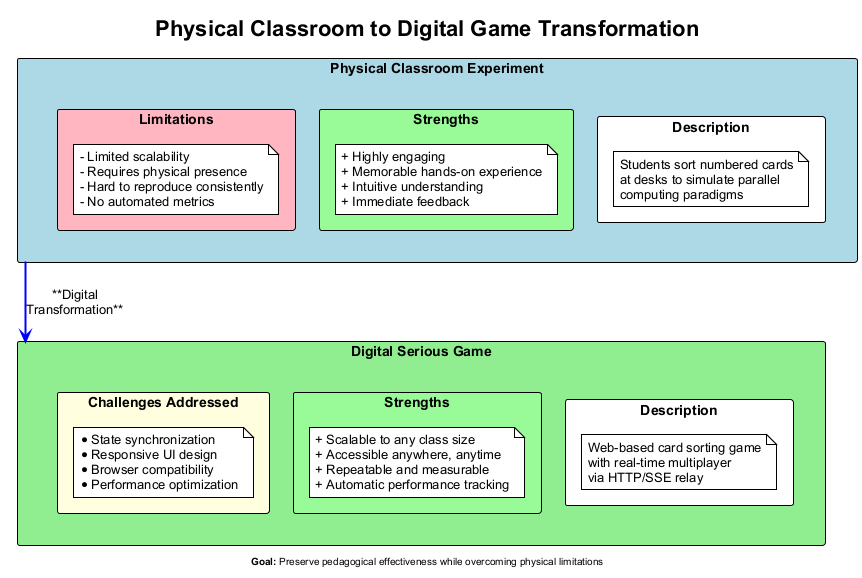
\includegraphics[width=0.85\textwidth]{figures/diagrams/physical-to-digital-mapping.png}
    \caption{Transformation from physical classroom activity to digital serious-game-based educational tool, preserving pedagogical effectiveness while overcoming physical limitations}
    \label{fig:physical-to-digital}
\end{figure}

%-----------------------------------------------------------------------
\section{Problem Statement}
\label{sec:problem-statement}

This thesis addresses the following research problem:

\begin{quote}
    \textit{How can we design and implement an effective web-based serious-game educational tool that teaches fundamental High-Performance Computing concepts (specifically OpenMP shared-memory parallelism and sequential vs. parallel execution) through interactive card-sorting while overcoming technical challenges of multiplayer state synchronization and responsive UI/UX constraints?}
\end{quote}

This overarching problem decomposes into three interrelated challenges:

\begin{itemize}
    \item \textbf{Educational Challenge}: How can abstract parallel computing concepts be mapped to concrete mechanics that accurately represent OpenMP paradigms?
    \item \textbf{Technical Challenge}: How can real-time multiplayer interaction be implemented across diverse devices with acceptable latency and consistent state?
    \item \textbf{Design Challenge}: How can we balance educational effectiveness with engagement and playability across different screen sizes and devices?
\end{itemize}

Detailed requirements analysis appears in Chapter~\ref{ch:methodology}.

%-----------------------------------------------------------------------
\section{Research Objectives}
\label{sec:objectives}

The primary objective of this thesis is to develop a functional serious-game-based educational tool that demonstrates the feasibility of teaching HPC concepts through web-based interactive activities, creating an open-source platform suitable for educational use and future research.

\subsection{Core Objectives}
\label{subsec:core-objectives}

\begin{enumerate}
    \item \textbf{Develop an Interactive Game-like Educational Tool}: Use card sorting as a metaphor for parallel sorting and OpenMP-style collaboration
    \item \textbf{Implement Web-First Functionality}: Run directly in modern browsers with responsive design
    \item \textbf{Create Multiplayer Capability}: Support many collaborative participants with synchronized shared state
    \item \textbf{Evaluate Technical Feasibility}: Assess architecture decisions and implementation challenges, including GDSync integration and HTTP/SSE relay networking
    \item \textbf{Support Instructor-Guided Use}: Ensure the artifact fits classroom and workshop workflows with facilitation and reflection
\end{enumerate}

%-----------------------------------------------------------------------
\section{Proposed Solution: HPC Sorting Serious Game}
\label{sec:proposed-solution}

This thesis presents the \textbf{HPC Sorting Serious Game}, a web-first serious-game-based educational tool for introducing parallel computing concepts through interactive card sorting. The card interaction model provides an intuitive bridge between concrete manipulation and abstract HPC concepts.
Technology selection process, alternatives explored, and final rationale are presented in Chapter~\ref{ch:methodology}.

%-----------------------------------------------------------------------
\section{Thesis Contributions}
\label{sec:contributions}

This thesis contributes to HPC education and educational game engineering in four areas:

\begin{enumerate}
    \item \textbf{Pedagogical Contribution}: A novel game-based approach for teaching OpenMP shared-memory parallelism and sequential vs. parallel execution comparison, directly inspired by successful physical classroom experiments, with systematic mapping between game mechanics and parallel computing paradigms. Additionally, demonstrates that fundamental HPC concepts can be taught effectively without requiring students to first master complex programming languages like C/C++, reducing cognitive load.
    \item \textbf{Technical Contribution}: A web-first implementation with synchronized multiplayer behavior and responsive UI for high-card-count interaction
    \item \textbf{Documentation Contribution}: Detailed discussion of practical engineering issues, including synchronization and framework constraints
    \item \textbf{Open-Source Contribution}: An extensible codebase that can be reused and expanded for future HPC education research
\end{enumerate}

Detailed discussion of these contributions appears in Chapter~\ref{ch:conclusion}.

%-----------------------------------------------------------------------
\section{Thesis Organization}
\label{sec:thesis-organization}

The remainder of this thesis is organized as follows:

\textbf{Chapter~\ref{ch:background}} reviews parallel computing fundamentals, serious games in education, web development constraints, and multiplayer architecture patterns.

\textbf{Chapter~\ref{ch:methodology}} describes the research method, requirements analysis, and technology selection.

\textbf{Chapter~\ref{ch:architecture}} presents system architecture, component design, networking model, and UI/UX strategy.

\textbf{Chapter~\ref{ch:implementation}} details implementation choices and key engineering decisions.

\textbf{Chapter~\ref{ch:problems}} analyzes development challenges and lessons learned.

\textbf{Chapter~\ref{ch:results}} presents system capabilities, technical performance, and preliminary educational observations.

\textbf{Chapter~\ref{ch:conclusion}} summarizes contributions and outlines future work.

\textbf{Appendices} provide supplementary materials including user documentation and technical references.

%-----------------------------------------------------------------------

% !TeX root = ../main.tex
\chapter{Background and Literature Review}
\label{ch:background}

This chapter provides the foundational knowledge and contextual background necessary to understand the HPC Sorting Serious Game. It reviews key concepts in parallel computing, serious games in education, web-based game development, and multiplayer networking architectures.

\begin{figure}[htbp]
    \centering
    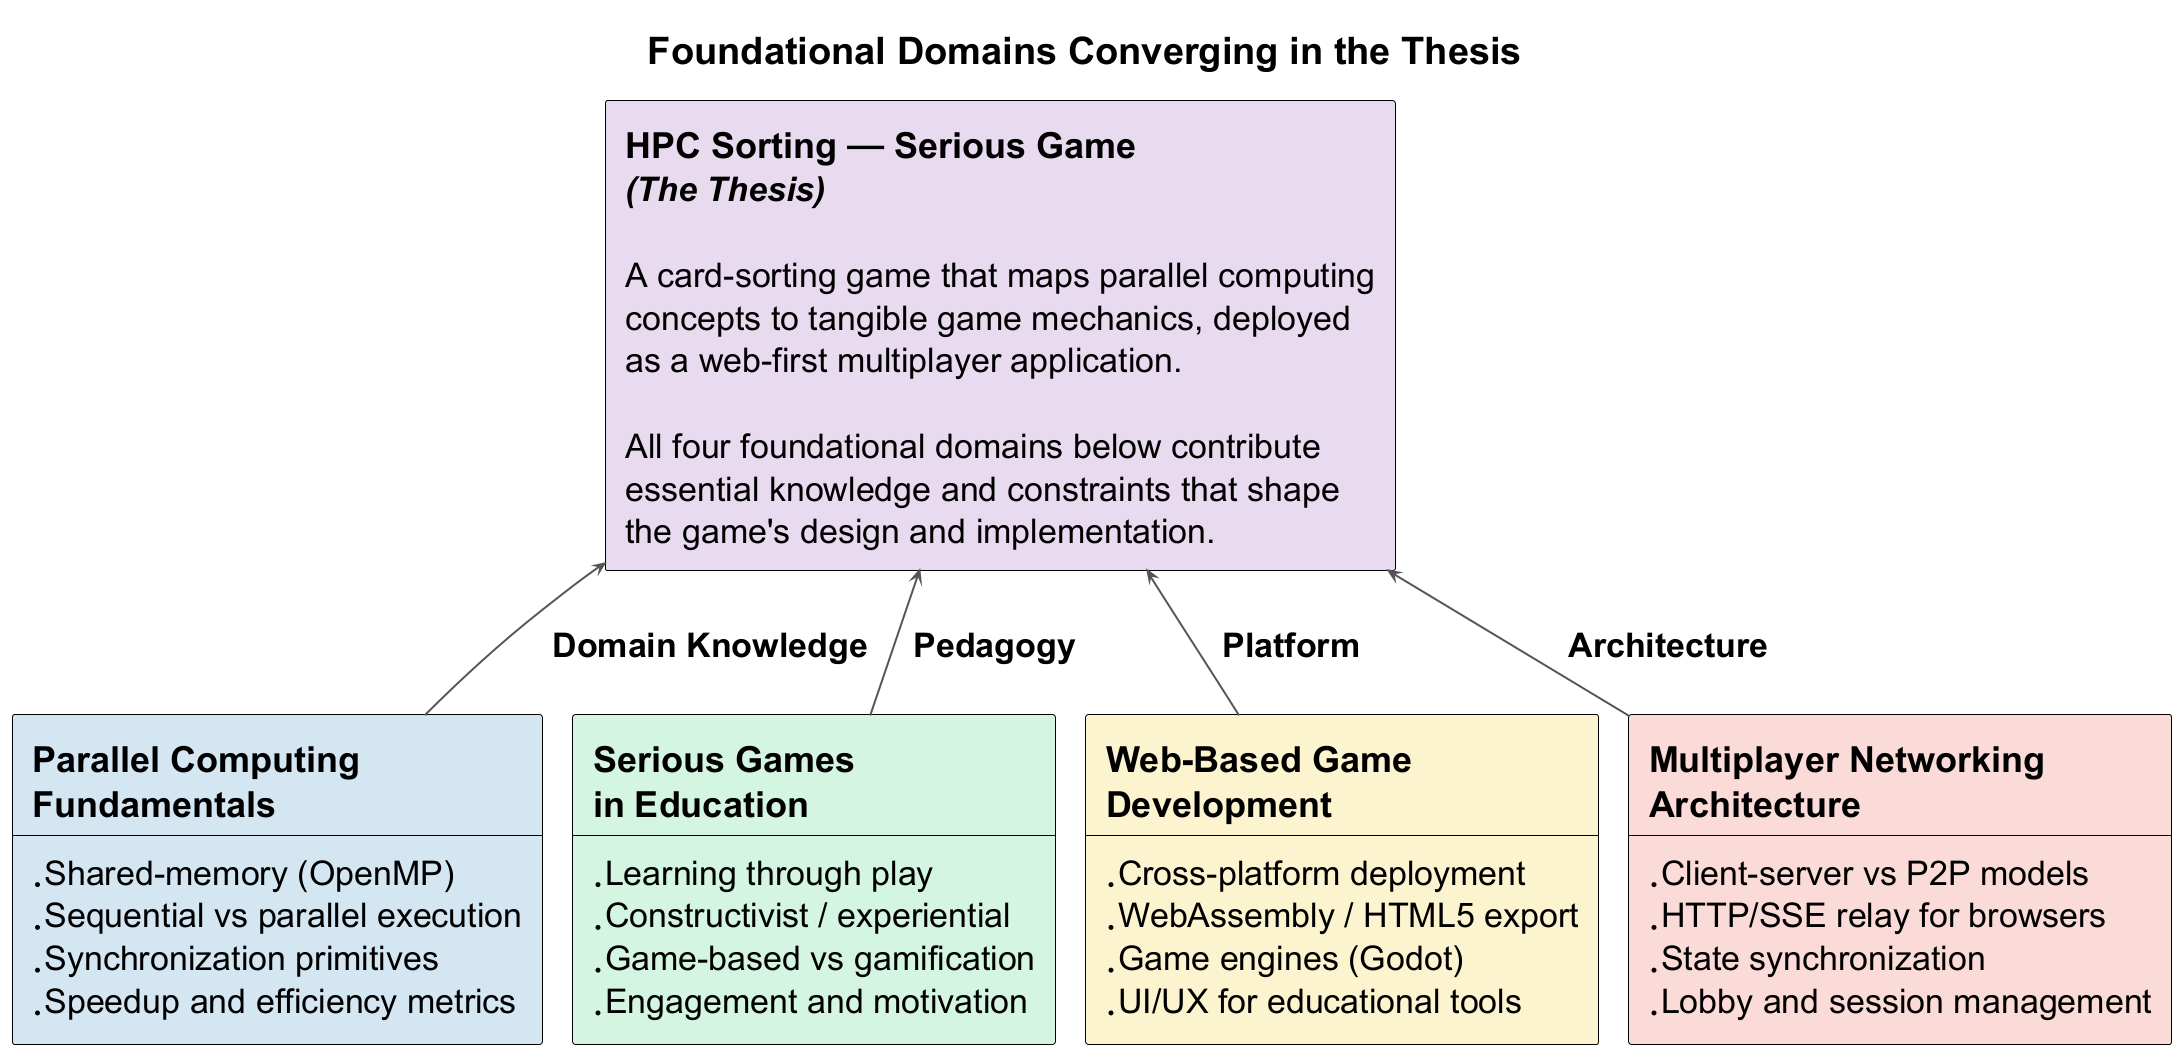
\includegraphics[width=0.95\textwidth]{figures/diagrams/background-concept-overview.png}
    \caption{Conceptual overview of the four knowledge domains converging in this thesis.}
    \label{fig:background-concept-overview}
\end{figure}

%-----------------------------------------------------------------------
\section{Parallel Computing Fundamentals}
\label{sec:parallel-computing}

Parallel computing is the simultaneous execution of multiple computational tasks to solve problems more efficiently than sequential processing. As Moore's Law approaches its physical limits, parallel computing has become essential for improving computational performance across scientific computing, data analytics, and real-time systems.

%-----------------------------------------------------------------------
\subsection{Parallel Programming Paradigms}
\label{subsec:parallel-paradigms}

Two primary paradigms dominate parallel computing education and practice: shared-memory parallelism and distributed-memory parallelism.

\subsubsection*{Shared-Memory Parallelism}

In shared-memory systems, multiple processors or cores access a common address space. All threads can read and write to the same memory locations, enabling efficient data sharing but requiring careful synchronization to prevent race conditions.

\textbf{Characteristics:}
\begin{itemize}
    \item All processors access the same physical memory
    \item Communication between threads occurs through shared variables
    \item Synchronization primitives (locks, barriers, atomic operations) prevent conflicts
    \item Lower communication overhead compared to distributed memory
    \item Scalability typically limited to a single workstation (one multi-core node)
\end{itemize}

\textbf{Applications:} Shared-memory parallelism is ideal for problems requiring frequent communication between processing units, such as iterative algorithms, graph processing, and data analytics on multicore processors.

\subsubsection*{Distributed-Memory Parallelism}

In distributed-memory systems, each processor has its own local memory. Processors communicate by explicitly sending and receiving messages over a network, requiring programmers to manage data distribution and communication patterns.

\textbf{Characteristics:}
\begin{itemize}
    \item Each processor has private memory space
    \item Communication between processes requires explicit message passing
    \item Scalable to thousands or millions of processors
    \item Higher communication overhead and latency
    \item No shared state eliminates race conditions but complicates programming
\end{itemize}

\textbf{Applications:} Distributed-memory parallelism is essential for large-scale scientific simulations, weather modeling, molecular dynamics, and big data processing across cluster and supercomputer architectures.

%-----------------------------------------------------------------------
\subsection{OpenMP: Shared-Memory Programming}
\label{subsec:openmp}

OpenMP (Open Multi-Processing) is a widely-used API for shared-memory parallel programming in C, C++, and Fortran. It uses compiler directives (pragmas) to specify parallel regions, enabling incremental parallelization of sequential code.

\textbf{Core Concepts:}
\begin{enumerate}
    \item \textbf{Parallel Regions}: Code sections executed by multiple threads simultaneously
    \item \textbf{Work-Sharing Constructs}: Distribute loop iterations or tasks among threads
    \item \textbf{Data Scoping}: Variables can be shared (visible to all threads) or private (thread-local copies)
    \item \textbf{Synchronization}: Barriers, critical sections, and atomic operations coordinate thread execution
    \item \textbf{Scheduling}: Strategies (static, dynamic, guided) control how iterations are assigned to threads
\end{enumerate}

\paragraph*{Example Code:}

\begin{lstlisting}[language=C++, caption={Simple OpenMP parallel loop}]
#pragma omp parallel for schedule(dynamic)
for (int i = 0; i < N; i++) {
    array[i] = compute_value(i);
}
\end{lstlisting}

\textbf{Educational Value:} OpenMP's simplicity makes it excellent for teaching parallel programming concepts. The incremental approach—starting with sequential code and adding pragmas—allows students to observe immediate performance improvements while learning about thread management, data dependencies, and race conditions.

%-----------------------------------------------------------------------
\subsection{MPI: Distributed-Memory Programming}
\label{subsec:mpi}

\begin{mdframed}[backgroundcolor=yellow!10, linecolor=orange, linewidth=2pt]
    \textbf{Note:} This section provides background on MPI for completeness and context within the broader HPC landscape. \textbf{The game implemented in this thesis focuses exclusively on OpenMP shared-memory parallelism.} MPI distributed-memory concepts are discussed here for educational context but are \textbf{not implemented} in the current version. See Chapter~\ref{ch:conclusion} for discussion of MPI as potential future work.
\end{mdframed}

MPI (Message Passing Interface) is the de facto standard for distributed-memory parallel programming. It provides a rich set of communication primitives for sending and receiving messages between processes, enabling scalable parallel computing on clusters and supercomputers.

\textbf{Core Operations:}
\begin{description}
    \item[Point-to-Point Communication] \texttt{MPI\_Send} and \texttt{MPI\_Recv} exchange messages between specific processes
    \item[Collective Communication] Operations like \texttt{MPI\_Bcast}, \texttt{MPI\_Gather}, and \texttt{MPI\_Reduce} involve all processes in a communicator
    \item[Process Groups] Communicators organize processes and define communication contexts
    \item[Data Types] MPI supports both primitive and user-defined data types for message content
\end{description}

\paragraph*{Example Code:}

\begin{lstlisting}[language=C++, caption={Simple MPI message passing}]
MPI_Init(&argc, &argv);
int rank, size;
MPI_Comm_rank(MPI_COMM_WORLD, &rank);
MPI_Comm_size(MPI_COMM_WORLD, &size);

if (rank == 0) {
    // Master process
    MPI_Send(data, count, MPI_INT, 1, 0, MPI_COMM_WORLD);
} else if (rank == 1) {
    // Worker process
    MPI_Recv(data, count, MPI_INT, 0, 0, MPI_COMM_WORLD, &status);
}

MPI_Finalize();
\end{lstlisting}

\textbf{Educational Value:} MPI teaches students about distributed computing challenges including data distribution, explicit communication, latency management, and scalability. The message-passing model forces programmers to think carefully about data ownership and communication patterns, skills essential for modern distributed systems.

%-----------------------------------------------------------------------
\subsection{Parallel Sorting Algorithms}
\label{subsec:parallel-sorting}

Sorting is a fundamental algorithmic problem that benefits significantly from parallelization. Several parallel sorting strategies exist, each with different communication and synchronization requirements.

\paragraph*{Parallel Merge Sort:}
\begin{itemize}
    \item Recursively divide array into subarrays
    \item Sort subarrays in parallel
    \item Merge sorted subarrays (potentially in parallel)
    \item Well-suited for shared-memory systems
    \item Time complexity: $O(\frac{n \log n}{p})$ with $p$ processors
\end{itemize}

\paragraph*{Parallel Quicksort:}
Parallel quicksort \citep{sanders2019sequential} exploits task-level parallelism through its recursive divide-and-conquer structure:
\begin{itemize}
    \item Select a \emph{pivot} element from the array
    \item \textbf{Partition} the array: elements $\leq$ pivot go left, elements $>$ pivot go right
    \item Recursively sort the left and right partitions \emph{in parallel} (each assigned to a different thread/task)
    \item Quality of the pivot determines load balance---a poor pivot creates unequal partitions
    \item Expected time complexity: $O\!\left(\frac{n \log n}{p}\right)$ with $p$ processors, assuming balanced pivots
\end{itemize}
Unlike merge sort, where the \emph{merge} phase is the synchronization bottleneck, quicksort's challenge is the \emph{partition} phase: threads must agree on a pivot and redistribute data before independent recursion can proceed. Parallel partitioning schemes (e.g., each thread partitions a local block, then a prefix-sum determines final positions) can parallelize this step, but at the cost of additional communication \citep{sanders2019sequential}.

\paragraph*{Sample Sort (MPI Pattern):}
\begin{itemize}
    \item Distribute data across processes
    \item Each process sorts local data
    \item Select sample elements to determine global pivots
    \item Redistribute data based on pivots
    \item Each process sorts its final partition
    \item Commonly used in distributed-memory systems
    \item \textit{Note: Not implemented in this thesis; discussed for context}
\end{itemize}

\textbf{Relevance to Educational Game:} The card-sorting game mechanics map directly to parallel sorting algorithms \citep{sanders2019sequential}. \emph{Parallel merge sort} maps to the game's divide-into-buffers, sort-locally, then merge-back workflow, with barriers separating each merge round. \emph{Parallel quicksort} maps to collaborative pivot selection and partitioning, followed by sub-group recursion into smaller card sub-arrays. In the implemented game, players act as threads (OpenMP) coordinating through shared memory to sort cards efficiently, making abstract algorithmic concepts tangible through gameplay. Chapter~\ref{ch:architecture} demonstrates how the existing algorithm-agnostic architecture already supports both strategies without code changes, and Chapter~\ref{ch:conclusion} outlines potential guided modes as medium-term extensions.

%-----------------------------------------------------------------------
\section{Serious Games in Education}
\label{sec:serious-games}

Serious games—games designed primarily for purposes beyond entertainment—have emerged as powerful educational tools. This section reviews the theoretical foundations and empirical evidence supporting game-based learning.

%-----------------------------------------------------------------------
\subsection{Definition and Characteristics}
\label{subsec:serious-games-definition}

\citet{zyda2005visual} defines a serious game as ``a mental contest, played with a computer in accordance with specific rules, that uses entertainment to further \textelp{} training, education, health, public policy, and strategic communication objectives.'' These games leverage game design principles to achieve learning objectives, skill development, or behavioral change.

\textbf{Key Characteristics:}
\begin{itemize}
    \item \textbf{Clear Learning Objectives}: Explicit educational goals aligned with curricula
    \item \textbf{Engaging Mechanics}: Game elements (challenges, rewards, feedback) maintain motivation
    \item \textbf{Active Learning}: Players learn by doing, not passive observation
    \item \textbf{Immediate Feedback}: Instant consequences of actions reinforce learning
    \item \textbf{Safe Experimentation}: Risk-free environment for trial and error
    \item \textbf{Progressive Difficulty}: Challenges scale with player skill development
\end{itemize}

%-----------------------------------------------------------------------
\subsection{Theoretical Foundations}
\label{subsec:game-based-learning-theory}

Game-based learning draws on several established educational theories:

\paragraph*{Constructivism:}

Constructivist theory \citep{piaget1970genetic} posits that learners actively construct knowledge through experience rather than passively receiving information. Games naturally support constructivist learning by placing players in problem-solving scenarios where they discover principles through experimentation.

\paragraph*{Flow Theory:}

\citet{csikszentmihalyi1990flow} describes ``flow'' as the optimal psychological state where challenge level matches skill level, producing deep engagement. Well-designed educational games maintain flow by dynamically adjusting difficulty, keeping learners challenged without overwhelming them.

\paragraph*{Experiential Learning:}

\citet{kolb1984experiential}'s experiential learning cycle---concrete experience, reflective observation, abstract conceptualization, active experimentation---aligns naturally with game mechanics. Players experience situations, observe outcomes, form hypotheses, and test them iteratively.

%-----------------------------------------------------------------------
\subsection{Empirical Evidence}
\label{subsec:serious-games-evidence}

Research consistently demonstrates the effectiveness of serious games for learning:

\paragraph*{\citet{connolly2012systematic} Meta-Analysis:}

A systematic literature review analysing 70 empirical studies found that serious games positively impact learning outcomes across multiple domains. Key findings include:

\begin{itemize}
    \item Improved knowledge acquisition and retention
    \item Enhanced perceptual and cognitive skills
    \item Increased motivation and engagement
    \item Better affective and motivational outcomes
    \item Most effective when integrated with traditional instruction
\end{itemize}

\paragraph*{\citet{papastergiou2009digital} Computer Science Education:}

A study of digital game-based learning in high school computer science found that students using educational games demonstrated:

\begin{itemize}
    \item Significantly higher knowledge acquisition
    \item Greater enjoyment and motivation
    \item Preference for game-based learning over traditional methods
    \item Improved attitudes toward computer science
\end{itemize}

%-----------------------------------------------------------------------
\subsection{Serious Games in Computer Science}
\label{subsec:games-cs-education}

Several successful serious games target computer science education.
\textbf{CodeCombat} \citep{codecombat} teaches programming through RPG-style gameplay in which players write real Python or JavaScript code to control characters; it is used in thousands of classrooms worldwide.
\textbf{Lightbot} \citep{lightbot} introduces sequencing, loops, and procedures through a visual puzzle interface that requires no programming syntax, making it accessible to young learners.

\paragraph*{Parallel Computing Games:}

In contrast to introductory programming, very few serious games target advanced topics like parallel computing education. Instructors typically rely on traditional, non-gamified software visualizers or simulation tools to teach parallel algorithm design, highlighting a significant gap in the current game-based learning landscape for advanced computer science topics.

%-----------------------------------------------------------------------
\subsection{Serious Games for HPC Education}
\label{subsec:serious-games-hpc}

High Performance Computing education faces unique challenges that serious games can address:

\paragraph*{Why Games for HPC?}

\begin{enumerate}
    \item \textbf{Abstract Concepts}: HPC involves invisible processes (threads, messages, synchronization) that are difficult to visualize through static diagrams
    \item \textbf{Temporal Dynamics}: Parallelism involves timing, race conditions, and coordination that unfold over time---games naturally model dynamic systems
    \item \textbf{Scale Mismatch}: Real HPC systems involve millions of operations per second; games can slow down and make these concepts observable
    \item \textbf{Hands-On Experience}: Students learn parallelism best by experiencing coordination challenges firsthand
\end{enumerate}

\paragraph*{Mapping HPC Concepts to Game Mechanics:}
The following mappings enable intuitive understanding of HPC concepts through gameplay (see Table~\ref{tab:hpc-game-mapping}).

\begin{table}[htbp]
    \centering
    \caption{HPC concepts mapped to game mechanics}
    \label{tab:hpc-game-mapping}
    \begin{tabular}{@{}l|l@{}}
        \toprule
        \textbf{HPC Concept}   & \textbf{Game Mechanic}                   \\
        \midrule
        Threads/Processes      & Players                                  \\
        \midrule
        Shared Memory          & Shared game board/container              \\
        \midrule
        Thread-Local Storage   & Private player inventory                 \\
        \midrule
        Synchronization        & Turn-taking or barriers                  \\
        \midrule
        Race Conditions        & Conflicting simultaneous actions         \\
        \midrule
        Speedup                & Time comparison (1 player vs. N players) \\
        \midrule
        Communication Overhead & Time to transfer items between players   \\
        \midrule
        Load Balancing         & Equal distribution of work               \\
        \bottomrule
    \end{tabular}
\end{table}

\paragraph*{Advantages of Game-Based HPC Learning:}

\begin{itemize}
    \item \textbf{No Prerequisites}: Students can experience parallel concepts before learning programming syntax
    \item \textbf{Misconception Surfacing}: Games reveal incorrect mental models (e.g., ``more threads always faster'')
    \item \textbf{Quantifiable Learning}: Performance metrics (time, moves) provide concrete feedback
    \item \textbf{Collaborative Learning}: Multiplayer games naturally create discussion and peer learning
    \item \textbf{Scalable Delivery}: Web-based games reach students regardless of institutional HPC infrastructure
\end{itemize}

%-----------------------------------------------------------------------
\section{Web-Based Game Development}
\label{sec:web-game-dev}

Web browsers provide a universal platform for educational game deployment, eliminating installation barriers and enabling access from any device with a modern browser.

%-----------------------------------------------------------------------
\subsection{Web Platform Advantages}
\label{subsec:web-advantages}

\textbf{Accessibility:} Web games require no installation—students access the game via URL, eliminating software distribution challenges and platform compatibility concerns.

\textbf{Cross-Platform:} A single web build runs on Windows, macOS, Linux, and even mobile browsers, maximizing reach with minimal development overhead.

\textbf{Instant Updates:} Deploying updates is immediate—no app store approval processes or user-initiated updates required.

\textbf{Low Barrier:} Modern browsers include powerful JavaScript engines, WebGL for graphics, and APIs for real-time communication.

%-----------------------------------------------------------------------
\subsection{Web Development Challenges}
\label{subsec:web-challenges}

\textbf{Browser Sandboxing:} Security restrictions prevent raw socket access, UDP communication, and local peer discovery—complicating multiplayer networking.

\textbf{Performance Overhead:} WebAssembly and JavaScript have overhead compared to native code, though performance is acceptable for 2D games.

\textbf{Networking Limitations:} Traditional peer-to-peer networking (like WebRTC data channels) can be complex to configure and may not work reliably across all network configurations.

%-----------------------------------------------------------------------
\subsection{Game Engines for Web}
\label{subsec:web-game-engines}

Several game engines support web deployment through HTML5/WebAssembly export, each with different trade-offs relevant to educational game development:
%TODO add links!
\begin{description}
    \item[Unity] offers a mature ecosystem with extensive documentation and asset store, but web exports tend to be large (50--100~MB) and the licensing model introduces constraints for open-source educational projects.
    \item[Unreal Engine] provides advanced rendering and networking capabilities; however, its focus on high-fidelity 3D and large export sizes make it less suited for lightweight 2D browser applications.
    \item[Godot Engine] is fully open-source (MIT license), produces compact web exports, and provides a Python-like scripting language (GDScript) alongside a scene-based architecture oriented toward rapid 2D development.
    \item[Cocos2d] is efficient for 2D applications and supports cross-platform builds, though its tooling ecosystem is smaller and the editor workflow is less integrated than some alternatives.
\end{description}

Key evaluation criteria for an educational web game include export size (affecting load time), 2D rendering quality, scripting accessibility for students who may inspect source code, and licensing compatibility with open educational resources. The engine selection process, evaluation evidence, and final decision are presented in Chapter~\ref{ch:methodology}, Section~\ref{subsec:godot-selection}.

%-----------------------------------------------------------------------
\section{Multiplayer Game Architecture}
\label{sec:bg-multiplayer-architecture}

Multiplayer functionality is essential for simulating OpenMP shared-memory parallelism with multiple players collaborating on shared data. This section reviews common multiplayer architectures and networking technologies.

\begin{figure}[htbp]
    \centering
    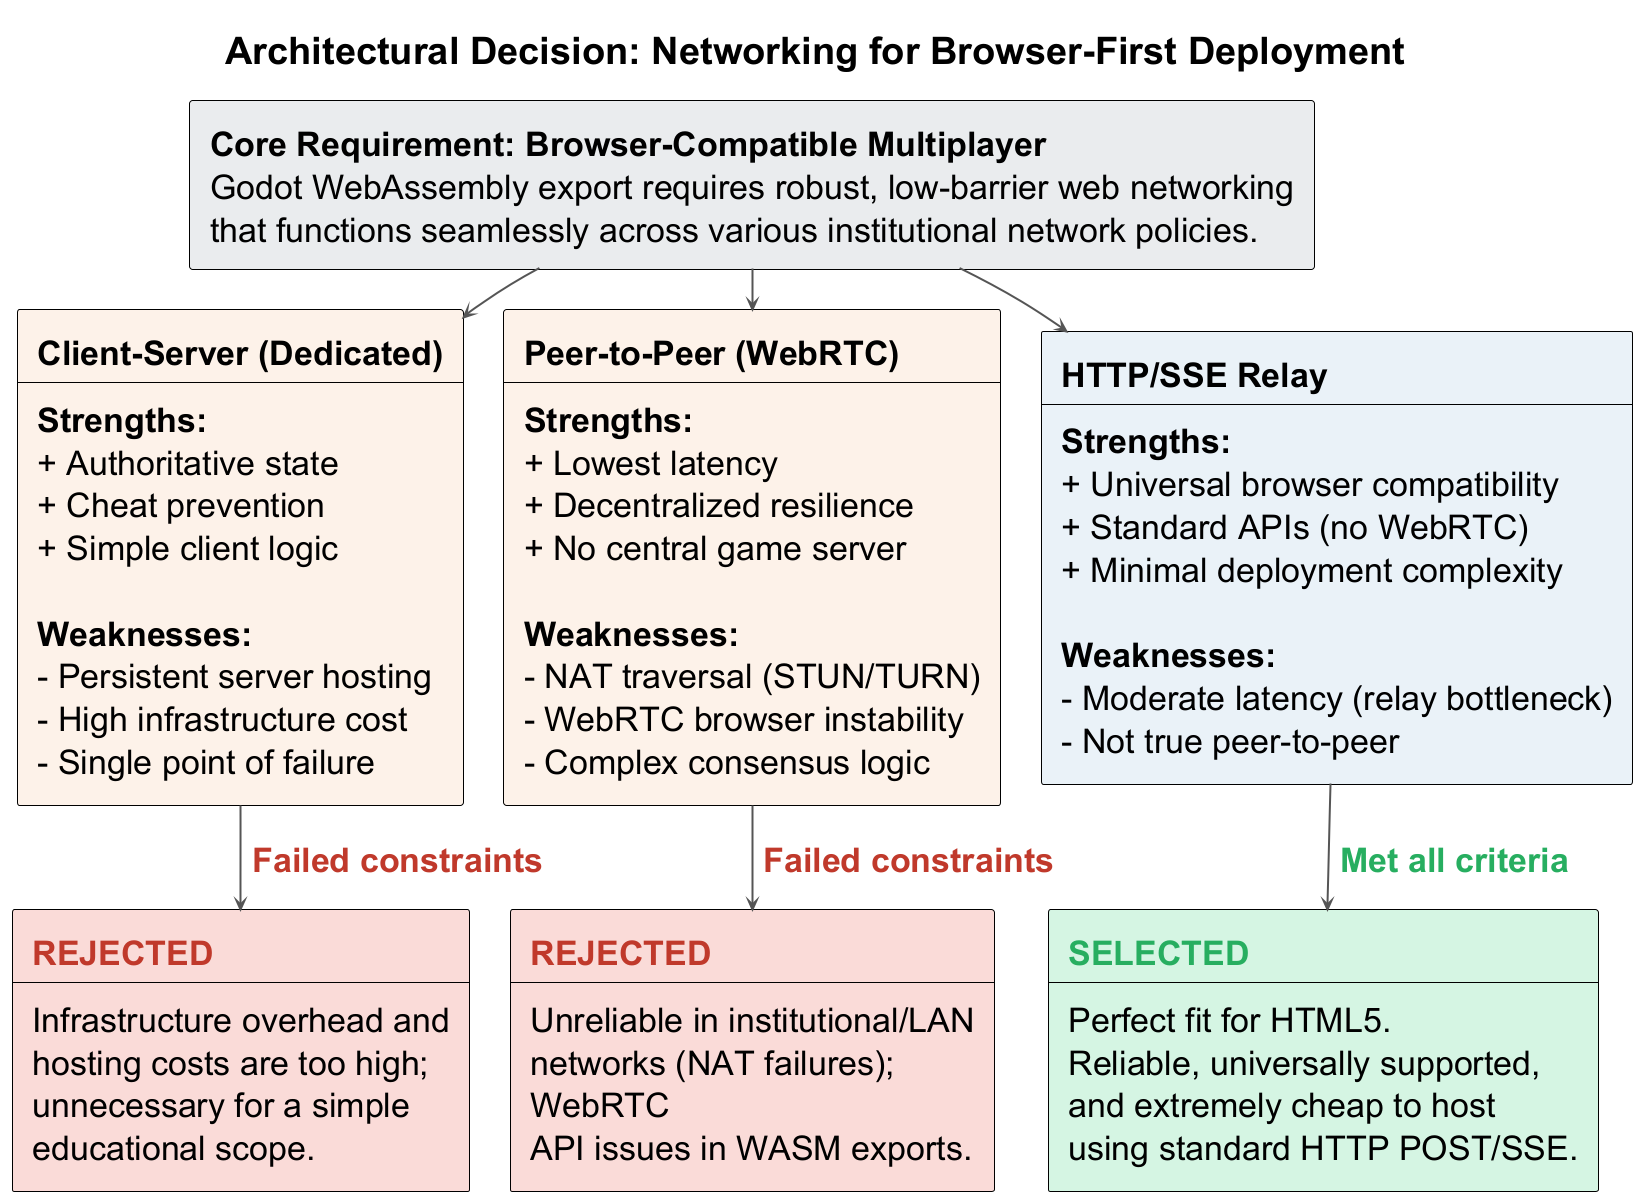
\includegraphics[width=0.95\textwidth]{figures/diagrams/networking-approach-comparison}
    \caption{Comparison of networking approaches for browser-first deployment, highlighting the HTTP/SSE relay selected for this thesis.}
    \label{fig:networking-approach-comparison}
\end{figure}

\begin{table}[htbp]
    \centering
    \caption{Summary matrix of networking approach evaluation criteria}
    \label{tab:networking-approach-summary}
    \small
    \begin{tabular}{@{}p{0.28\textwidth}p{0.2\textwidth}p{0.2\textwidth}p{0.2\textwidth}@{}}
        \toprule
        \textbf{Evaluation Criteria} & \textbf{Client-Server} & \textbf{P2P (WebRTC)} & \textbf{HTTP/SSE Relay} \\
        \midrule
        Browser compatibility        & Partial                & Problematic           & \textbf{Universal}      \\
        Infrastructure needs         & High                   & Low (STUN/TURN)       & \textbf{Minimal}        \\
        Implementation complexity    & Medium                 & High                  & \textbf{Low}            \\
        Latency                      & Low                    & Lowest                & Moderate                \\
        \bottomrule
    \end{tabular}
\end{table}

%-----------------------------------------------------------------------
\subsection{Client-Server Architecture}
\label{subsec:client-server}

In a traditional client-server model, a dedicated server hosts the authoritative game state. Clients send their inputs to the server, which validates actions, updates the canonical state, and broadcasts the result to all connected clients. This architecture provides strong consistency guarantees and inherent cheat prevention, since no client can unilaterally alter the game state. However, it requires maintaining dedicated server infrastructure, introduces a single point of failure, and routes all communication through the server, adding latency to every interaction. These costs are justified in scenarios where state correctness is paramount, but they impose operational overhead that may be disproportionate for small-scale educational deployments.

%-----------------------------------------------------------------------
\subsection{Peer-to-Peer Architecture}
\label{subsec:p2p}

Peer-to-peer (P2P) networks eliminate the need for a dedicated server by allowing clients to communicate directly. One peer is typically designated as ``host'' to serve as the authority for conflict resolution. This approach removes server infrastructure costs and can reduce latency for direct connections between nearby peers. However, establishing connections is considerably more complex due to NAT traversal requirements, and the host peer bears a disproportionate performance burden. Cheat prevention is also more difficult, since clients have more control over state. P2P topologies scale well for small groups (2--8 players) but become impractical as group size increases due to the quadratic growth in connection count.

%-----------------------------------------------------------------------
\subsection{Web Transport Technologies}
\label{subsec:web-transport}

Web browsers offer several options for real-time communication, each with trade-offs:

\paragraph*{HTTP Polling} is the simplest approach: the client repeatedly requests updates from the server at fixed intervals. It is universally supported and trivial to implement, but incurs higher latency and server load due to the frequency of requests, making it suitable only for low-frequency state updates.

\paragraph*{Server-Sent Events (SSE)} allow the server to push events to the client over a persistent HTTP connection. SSE is simpler than WebSocket (it uses standard HTTP with no protocol upgrade), supports automatic reconnection through the browser API, and enjoys broad proxy compatibility. The trade-off is that the channel is unidirectional---server to client only---so client-to-server communication must use a separate mechanism such as HTTP POST.

\paragraph*{HTTP + SSE Relay Architecture:}

For web-based multiplayer games requiring broad browser compatibility, a relay server architecture using HTTP POST for client-to-server communication and SSE for server-to-client events provides:

\begin{itemize}
    \item Universal browser support without WebSocket complexity
    \item Works through firewalls and proxies that block WebSocket
    \item Simplified connection establishment (no STUN/TURN required)
    \item Trade-off: All traffic routes through server (no P2P)
    \item Acceptable latency for turn-based or slower-paced games
\end{itemize}

%-----------------------------------------------------------------------
\subsection{State Synchronization Patterns}
\label{subsec:state-sync}

Maintaining consistent game state across multiple clients is challenging. Common patterns include:

\paragraph*{Deterministic Lockstep}
requires all clients to simulate identical game logic, with inputs synchronized and executed simultaneously. This guarantees identical state on every client but is highly sensitive to latency and packet loss, making it most suitable for real-time strategy games (e.g., \textit{Age of Empires}, \textit{StarCraft}).

\paragraph*{Client-Side Prediction}
allows clients to predict the results of their own actions immediately, while the server validates and corrects if necessary. This provides a responsive feel despite latency, at the cost of occasional reconciliation when predictions are wrong. First-person shooters such as \textit{Counter-Strike} and \textit{Overwatch} rely on this technique.

\paragraph*{Authoritative Server/Host}
models maintain a single canonical state on the server or host. Clients send proposed actions and receive authoritative state updates in return. This approach is simpler to implement and reason about, provides stronger consistency, and is well-suited for turn-based or slower-paced games where moderate latency is acceptable.

\paragraph*{Suitability for Educational Games:}

For educational multiplayer games where correctness and pedagogical clarity take priority over competitive low-latency performance, the \textbf{authoritative server/host} model is a natural fit: it is straightforward to implement, prevents inconsistencies across clients, and aligns with centralized coordination patterns found in parallel computing. The specific synchronization model adopted for this thesis is discussed in Chapter~\ref{ch:methodology}.

%-----------------------------------------------------------------------
\section{Related Work}
\label{sec:related-work}

This section reviews existing educational tools and games related to parallel computing and serious games.

%-----------------------------------------------------------------------
\subsection{Parallel Computing Educational Tools}
\label{subsec:parallel-tools}

Several tools exist for teaching parallel computing, each with strengths and limitations.
\textbf{PARMACS} provides parallel algorithm visualization through thread and process execution timelines, but offers limited interactivity and runs only on desktop platforms.
Tools such as \textbf{Intel VTune} and \textbf{TAU} (Tuning and Analysis Utilities) focus on OpenMP performance profiling; while powerful, they have steep learning curves and are designed for optimization work rather than introductory education.
\textbf{MPICH} and \textbf{Open MPI} supply debugging tools for MPI-based programs, but require cluster access or virtual machines and presuppose programming ability.

\paragraph*{Gap Identification:}

Existing tools generally fall into two categories: (1)~visualization tools that show parallel execution but lack hands-on interaction, and (2)~programming environments that require coding skills, deterring beginners. Few tools bridge the gap between conceptual understanding and practical implementation, and fewer still are designed for web platforms or incorporate game mechanics to enhance engagement.

%-----------------------------------------------------------------------
\subsection{Serious Games for Computing Education}
\label{subsec:cs-games}

Several serious games have successfully taught computing concepts, though none specifically target OpenMP-style parallel computing on web platforms.
\textbf{CodeCombat} teaches programming through RPG gameplay in which players write real Python or JavaScript; it is effective for syntax and basic algorithms but does not address parallelism.
\textbf{Human Resource Machine} uses visual assembly-like puzzles to teach sequential algorithmic thinking without syntax barriers, but its single-threaded model excludes parallelism concepts.
\textbf{Shenzhen I/O} targets hardware design and low-level optimization for experienced programmers; while sophisticated, it has no explicit parallel computing focus.

\paragraph*{Gap in Parallel Computing Games:}

No widely-adopted serious game specifically teaches parallel computing concepts like OpenMP shared-memory parallelism through interactive, game-based mechanics on web platforms. This gap motivated the development of the HPC Sorting Serious Game, which focuses on OpenMP concepts with potential for future MPI extensions.

%-----------------------------------------------------------------------
\subsection{Physical Teaching Methods}
\label{subsec:physical-methods}

The pedagogical approach for this thesis draws inspiration from physical classroom activities:

\paragraph*{CS Unplugged:}

The CS Unplugged collection teaches computer science concepts---algorithms, sorting, searching---through hands-on activities that require no computers. These activities are highly engaging but inherently limited to in-person classroom settings and are difficult to scale or reproduce consistently.

\paragraph*{Professor D'Agostino's Card Sorting Experiments:}

As described in Chapter~\ref{ch:introduction}, Professor Daniele D'Agostino conducted classroom experiments where students physically sorted numbered cards to simulate parallel computing paradigms. These experiments demonstrated:

\begin{itemize}
    \item High student engagement and retention
    \item Intuitive understanding of parallelism concepts
    \item Memorable hands-on experience
    \item Clear differentiation between sequential and parallel execution models
\end{itemize}

However, physical experiments have limitations:

\begin{itemize}
    \item Require physical classroom presence
    \item Not scalable to large classes
    \item Difficult to reproduce consistently
    \item Limited flexibility in parameters (card count, student count)
    \item No performance metrics or automated feedback
\end{itemize}

\paragraph*{Digital Transformation:}

This thesis aims to capture the pedagogical effectiveness of physical card-sorting experiments in a digital, web-first serious game that overcomes the limitations of physical activities while preserving their educational benefits.

%-----------------------------------------------------------------------
\section{Summary}
\label{sec:background-summary}

This chapter established the foundational knowledge necessary to understand the HPC Sorting Serious Game:

\begin{itemize}
    \item \textbf{Parallel Computing}: Reviewed OpenMP shared-memory parallelism (the focus of this thesis) and MPI distributed-memory paradigms (for context), highlighting their educational challenges and importance.

    \item \textbf{Serious Games}: Examined theoretical foundations, empirical evidence, and successful examples of game-based learning in computer science education.

    \item \textbf{Web Development}: Discussed advantages and challenges of web platforms for educational games, and surveyed available game engines with web export capabilities.

    \item \textbf{Multiplayer Architecture}: Compared client-server and peer-to-peer models, introduced web transport technologies (HTTP/SSE), and justified the host-authoritative approach for OpenMP simulation.

    \item \textbf{Related Work}: Identified gaps in existing parallel computing educational tools and serious games, motivating the development of this project.
\end{itemize}

The next chapter describes the research methodology, requirements analysis, and technology selection decisions that guided the development of the HPC Sorting Serious Game.

% !TeX root = ../main.tex
\chapter{Methodology}
\label{ch:methodology}

This chapter describes the research methodology, requirements analysis, design approach, and technology selection decisions that guided the development of the HPC Sorting Serious Game. The methodology follows a Design Science Research approach, emphasizing iterative development and evaluation.

%-----------------------------------------------------------------------
\section{Research Methodology}
\label{sec:research-methodology}

%-----------------------------------------------------------------------
\subsection{Design Science Research Framework}
\label{subsec:design-science}

This thesis adopts the Design Science Research (DSR) methodology \citep{hevner2004design, peffers2007design}, which is particularly well-suited for developing innovative artifacts that address practical problems while contributing to theoretical knowledge.

\paragraph*{DSR Process Model:}

The DSR process consists of six iterative activities:

\begin{enumerate}
    \item \textbf{Problem Identification and Motivation}: Identify the research problem (teaching HPC concepts) and justify the value of a solution (web-based serious game).

    \item \textbf{Define Objectives of a Solution}: Infer solution objectives from problem definition and existing knowledge (create engaging, accessible, educational multiplayer game).

    \item \textbf{Design and Development}: Create the artifact (HPC Sorting Serious Game) by selecting appropriate technologies and implementing game mechanics.

    \item \textbf{Demonstration}: Demonstrate the artifact's utility by applying it to the problem context (students learning parallel computing).

    \item \textbf{Evaluation}: Observe and measure how well the artifact supports a solution to the problem (usability testing, performance benchmarking).

    \item \textbf{Communication}: Communicate the problem, artifact, evaluation, and contributions to relevant audiences (thesis, potential publications).
\end{enumerate}

\paragraph*{Rationale for DSR:}

DSR is appropriate for this research because:

\begin{itemize}
    \item The goal is to create a functional artifact (serious game) rather than merely analyze existing phenomena
    \item The problem is practical and relevant to HPC education
    \item The solution requires integrating knowledge from multiple domains (pedagogy, game design, parallel computing, web development)
    \item Evaluation can be both utility-based (does it work?) and design-based (is it well-constructed?)
\end{itemize}

\section{Requirements Analysis}
\label{sec:requirements}

A comprehensive requirements analysis was conducted to ensure the game met educational and functional objectives.

%-----------------------------------------------------------------------
\subsection{Educational Requirements}
\label{subsec:educational-requirements}

The primary purpose of the game is education. Requirements were derived from HPC learning objectives and parallel computing curricula:

\paragraph*{ER1: OpenMP Simulation}
\begin{itemize}
    \item The game must simulate shared-memory parallelism
    \item All players must see all cards in the main container (shared memory)
    \item Players must have public buffers (partitioned shared memory for per-thread work)
    \item No explicit communication required between players (implicit synchronization)
\end{itemize}

\paragraph*{ER2: Sequential Execution Baseline}
\begin{itemize}
    \item The game must provide a single-player mode for sequential execution comparison
    \item A single player must sort all cards without parallelism
    \item This mode serves as a baseline for understanding speedup from parallelization
    \item Players should be able to compare sequential vs. parallel performance
\end{itemize}

\paragraph*{ER3: Performance Feedback}
\begin{itemize}
    \item The game must provide timing information (simulating speedup measurement)
    \item Move counting must encourage algorithmic efficiency
    \item Visual feedback must reinforce correct and incorrect actions
\end{itemize}

\paragraph*{ER4: Progressive Difficulty}
\begin{itemize}
    \item Support variable numbers of cards (10--200) for scalability lessons
    \item Support variable numbers of players (10--40) for parallelism degree
    \item Provide different sorting challenges (random, partially sorted, reverse sorted)
\end{itemize}

\paragraph*{ER5: Conceptual Clarity}
\begin{itemize}
    \item Game mechanics must clearly map to HPC concepts
    \item Visual design must distinguish shared vs. private data
    \item Terminology should align with parallel computing vocabulary when appropriate
\end{itemize}

%-----------------------------------------------------------------------
\subsection{Functional Requirements}
\label{subsec:functional-requirements}

Functional requirements specify what the system must do:

\paragraph*{FR1: Card Management}
\begin{itemize}
    \item Generate configurable numbers of cards with unique values
    \item Shuffle cards randomly at game start
    \item Render cards with clear visual representation (number, state)
    \item Support dragging and dropping cards between containers
\end{itemize}

\paragraph*{FR2: Single-Player Mode}
\begin{itemize}
    \item Provide a single-player game mode representing sequential execution
    \item Display all cards in a scrollable container
    \item Provide work buffer zones for temporary storage
    \item Validate sorting order upon completion
    \item Display completion time and move count
\end{itemize}

\paragraph*{FR3: Multiplayer Mode}
\begin{itemize}
    \item Enable 10--40 players to connect via server-relayed networking
    \item Provide lobby for matchmaking and game configuration
    \item Display shared container visible to all players (OpenMP shared memory)
    \item Synchronize card movements across all clients
    \item Provide public buffers for each player (partitioned shared memory for per-thread sorting)
    \item Hide cards in other players' public buffers (thread-private data)
    \item Handle player disconnections gracefully
\end{itemize}

\paragraph*{FR4: User Interface}
\begin{itemize}
    \item Main menu with navigation to single-player and multiplayer modes
    \item Lobby interface for creating/joining games
    \item In-game UI with timer, move counter, player indicators
    \item Victory screen with performance summary
    \item Settings for theme, controls, and game parameters
\end{itemize}

\paragraph*{FR5: Feedback Systems}
\begin{itemize}
    \item Toast notifications for events (player joined, card moved, errors)
    \item Visual animations for card pickup, drop, invalid moves
    \item Sound effects for actions (optional, can be disabled)
    \item Confetti or celebration effects upon game completion
          % TODO: [Artifact] Completion-state feedback screenshot with annotations.
          % TODO: [Purpose] Show how celebration feedback reinforces task completion and user feedback loops.
          % TODO: [Source Inputs] End-of-game UI state capture (confetti/celebration, timer, move summary, and completion labels).
          % TODO: [Placement] Near FR5 or in results chapter screenshot montage if consolidated.
          % TODO: [Done Criteria] Annotate which visual/audio channel corresponds to completion confirmation.
          % TODO: [Cross-refs] Chapter~\ref{ch:results}, Sections~\ref{subsec:functional-features},~\ref{subsec:engagement-effects}, and~\ref{sec:usability-evaluation}.
\end{itemize}

\paragraph*{FR6: Quality Attributes}
\begin{itemize}
    \item Target 60 FPS in modern web browsers
    \item Game initialization and card generation under 2 seconds
    \item Support up to 200 cards without significant performance degradation
    \item Intuitive interface requiring no tutorial for basic gameplay
    \item Responsive drag-and-drop with visual feedback
    \item Graceful handling of network disconnections
    \item Clean code structure with modular design
    \item Open-source license (MIT) for educational reuse
    \item No account creation or authentication required
\end{itemize}


\subsection{Core Concept}
\label{subsec:core-concept}

The game presents players with a deck of numbered cards that must be sorted in ascending order. This simple metaphor maps directly to parallel sorting algorithms, with different game modes representing different execution paradigms:

\paragraph*{Single-Player Mode (Sequential Execution):} Represents traditional sequential algorithm execution where a single process sorts all data. The player works alone with all cards visible, performing the entire sorting task independently.

\paragraph*{Multiplayer Mode (OpenMP Shared-Memory Parallelism):} Represents shared-memory parallelism where multiple threads cooperate on a single address space. All players work collaboratively with cards visible in a shared container (representing shared memory), each player uses public buffer zones for local sorting (representing partitioned regions of shared memory), and players work simultaneously without forced turn-taking (representing OpenMP's implicit synchronization and parallel execution model).

The complete architecture and pedagogical mapping are detailed in Chapter~\ref{ch:architecture}.

\begin{figure}[htbp]
    \centering
    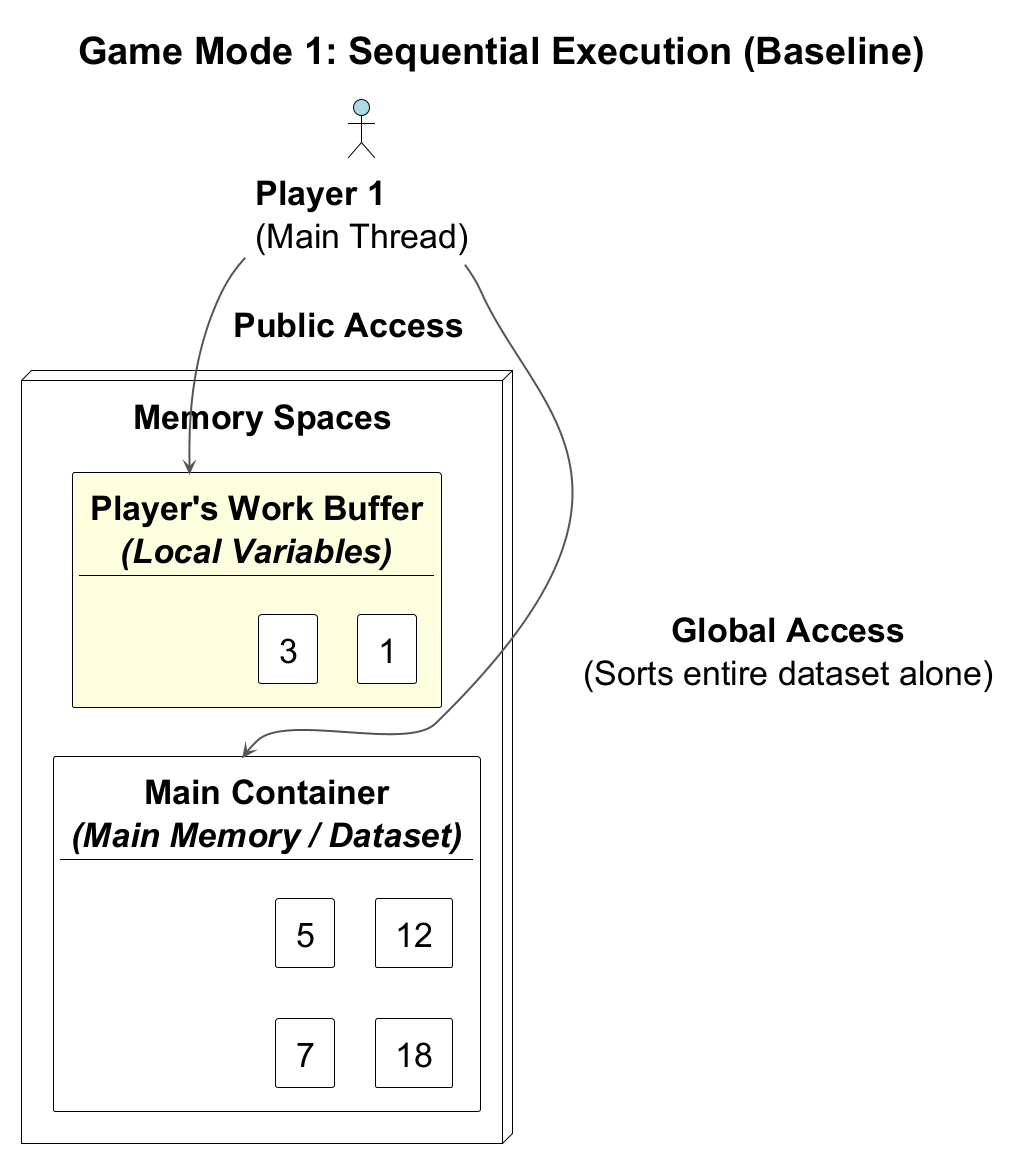
\includegraphics[width=0.65\textwidth]{figures/diagrams/sequential-mode.png}
    \caption{Game Mode~1: Sequential Execution (Baseline). A single player (main thread) sorts the entire dataset alone, accessing both the main container (main memory) and a public work buffer (local variables).}
    \label{fig:sequential-mode}

    \vspace{0.3em}
    \begin{description}
        \item[Pedagogical mapping:] A single actor represents a single CPU thread that processes the array element-by-element. No parallel speedup occurs; this mode serves as the baseline ($T_1$) for calculating parallel efficiency.
    \end{description}
\end{figure}

\begin{figure}[htbp]
    \centering
    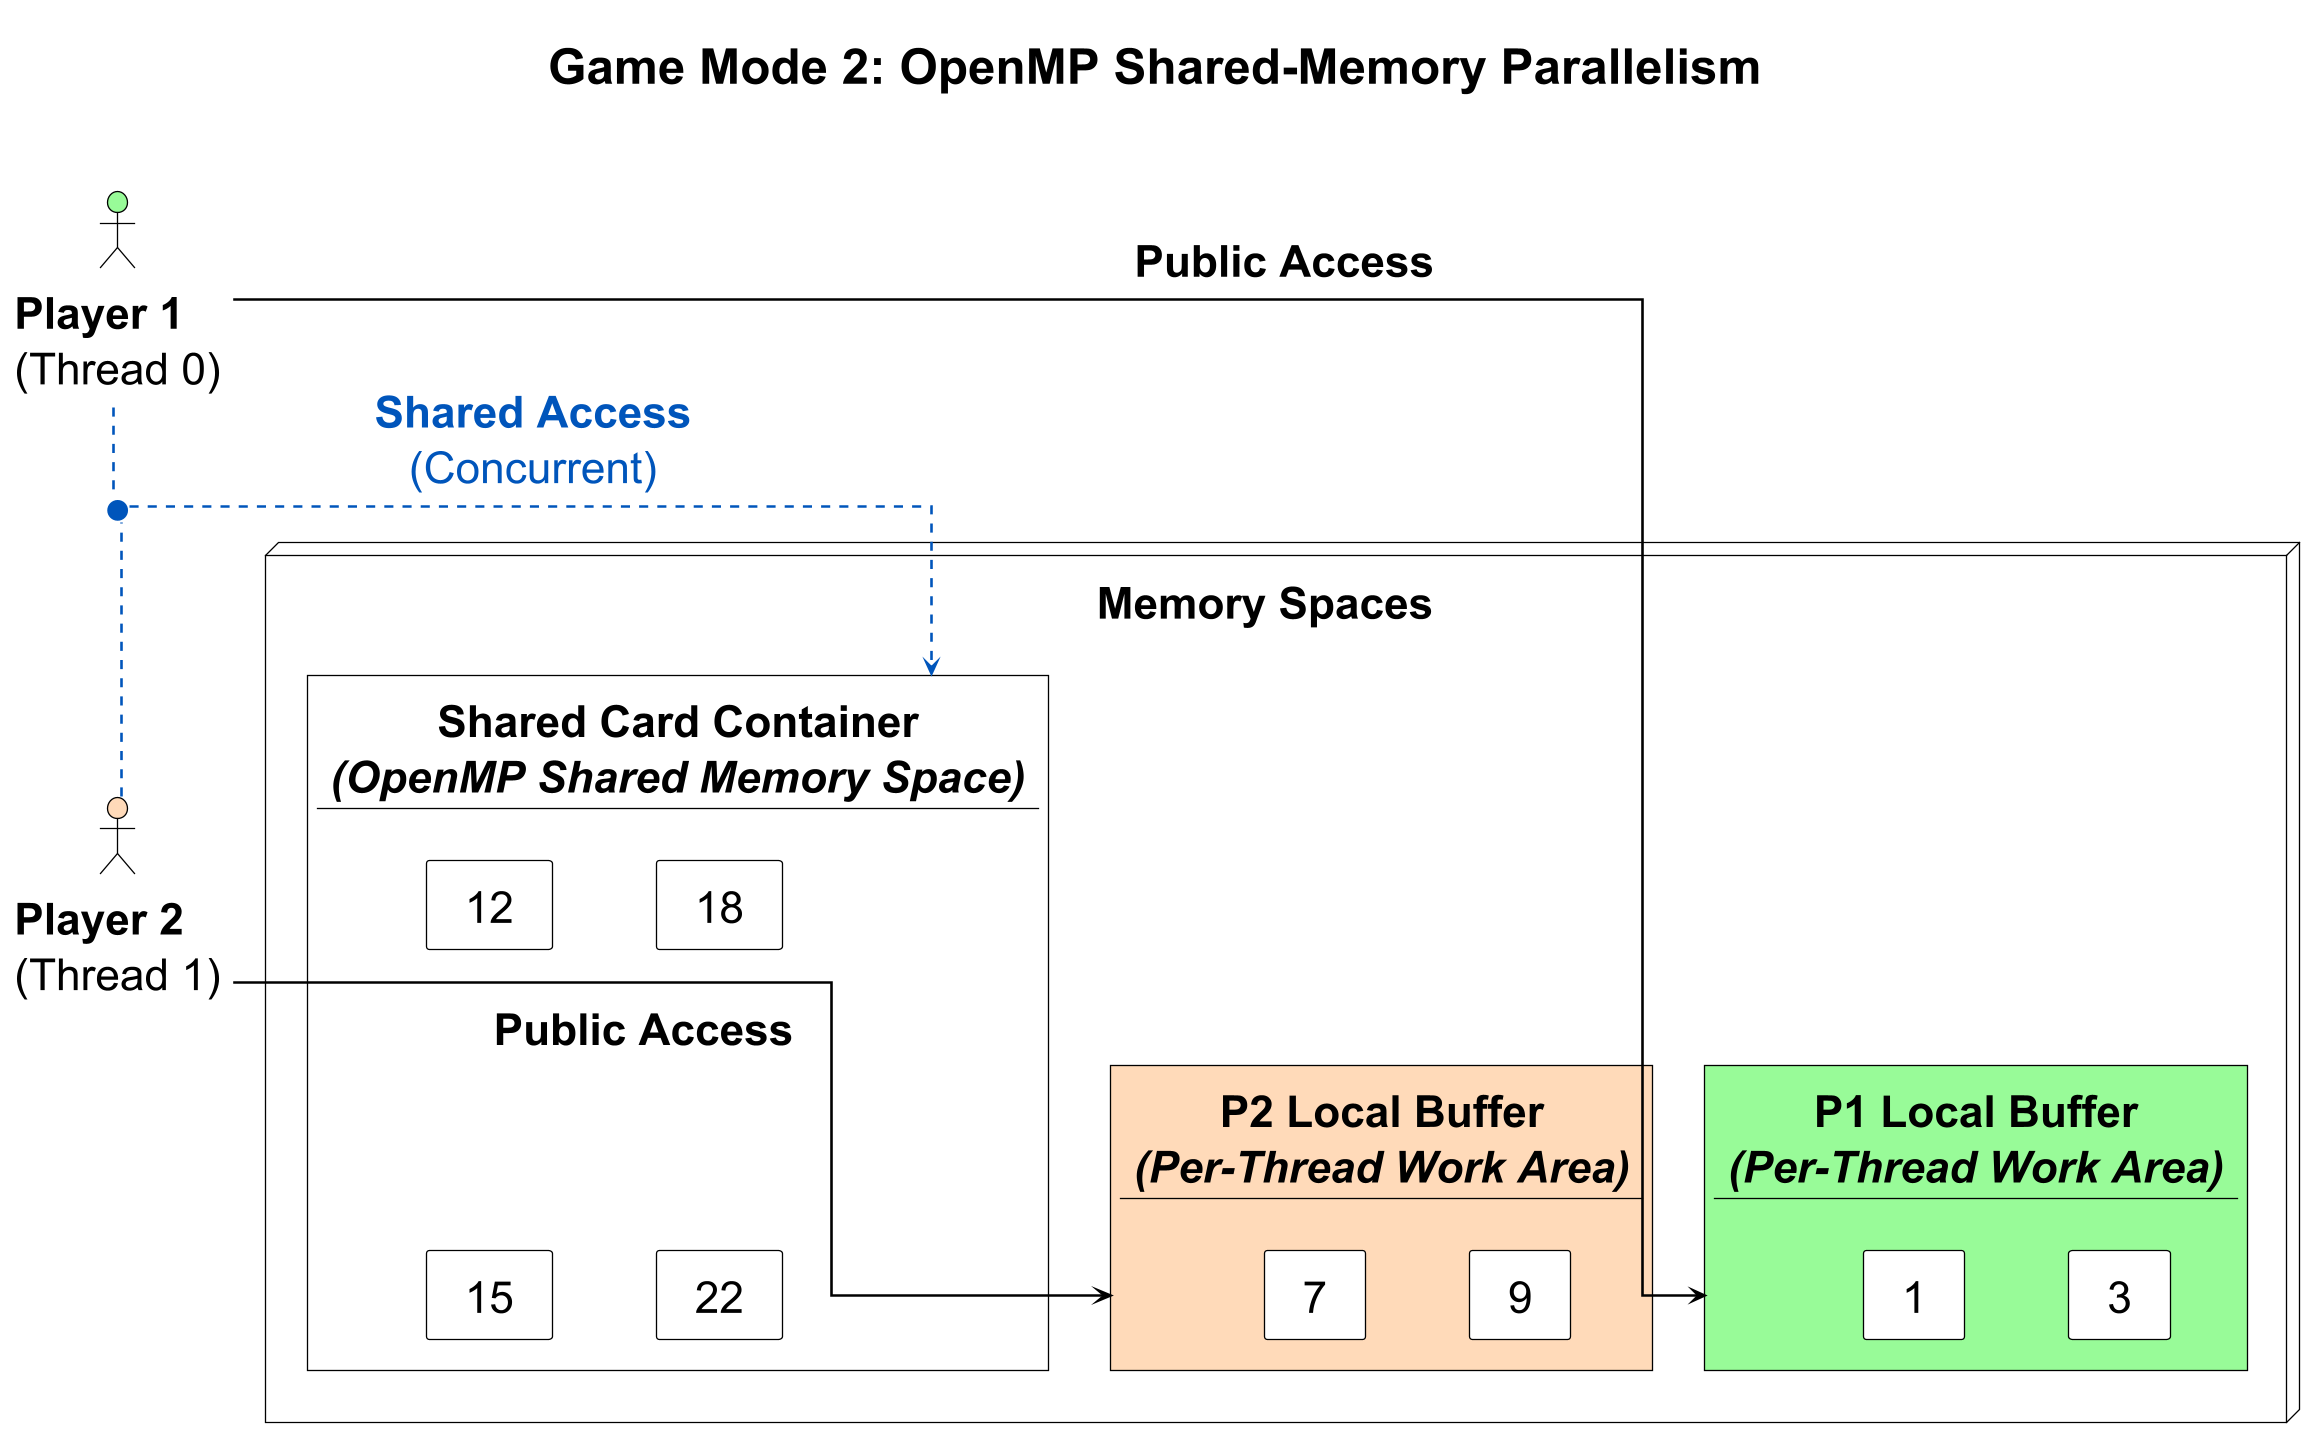
\includegraphics[width=0.85\textwidth]{figures/diagrams/openmp-mode.png}
    \caption{Game Mode~2: OpenMP Shared-Memory Parallelism. Multiple players (threads) access a shared card container concurrently and use public buffers for per-thread sorting.}
    \label{fig:openmp-mode}

    \vspace{0.3em}
    \begin{description}
        \item[Pedagogical mapping:] \textbf{Players} represent concurrent threads working on a single task. The \textbf{shared container} models a globally accessible memory space, introducing concepts such as race conditions and the need for synchronization (barriers). \textbf{Public buffers} represent partitioned regions of shared memory---analogous to per-thread segments of a shared array (e.g., \texttt{array[tid*chunk ..\ (tid+1)*chunk-1]}), where each thread conventionally works on its own portion while the data remains technically accessible to all threads. This models common OpenMP patterns such as block-based parallel sorting, where each thread sorts a local chunk before results are merged back into the shared space.
    \end{description}
\end{figure}

%-----------------------------------------------------------------------
\section{Technology Selection}
\label{sec:technology-selection}

Technology choices were treated as methodological outcomes of iterative experimentation, not fixed assumptions. This section documents the evaluation process, alternatives explored, observed constraints, and final decisions for both core architecture and the supporting development toolchain.

%-----------------------------------------------------------------------
\subsection{Tool and Framework Evaluation Process}
\label{subsec:tool-eval-process}

Selection decisions were made using a consistent set of criteria aligned with thesis goals:
\begin{itemize}
    \item \textbf{Educational fit}: ability to support clear mapping between gameplay mechanics and HPC concepts
    \item \textbf{Web deployment feasibility}: practical browser support and export reliability
    \item \textbf{Multiplayer support}: synchronization model maturity and debugging feasibility
    \item \textbf{Ecosystem maturity}: documentation quality, examples, and community responsiveness
    \item \textbf{Debugging observability}: runtime inspection and logging support
    \item \textbf{Development speed}: iteration time and implementation complexity
    \item \textbf{Maintainability}: modularity, replacement cost, and long-term project sustainability
\end{itemize}

Decisions were validated through prototype iterations described in Section~\ref{subsec:development-approach}, with problematic assumptions revisited as implementation evidence emerged.

%-----------------------------------------------------------------------
\subsection{Game Engine: Godot 4.x}
\label{subsec:godot-selection}

\paragraph*{Alternatives explored:}

Unity, Unreal, Godot, and Cocos2d were evaluated against the criteria in Section~\ref{subsec:tool-eval-process}.

\paragraph*{Practical background and evaluation context:}
Before this thesis, the author had only brief prior hands-on exposure to Unity and Godot, and no production experience with Unreal or Cocos2d. For this reason, engine selection emphasized thesis-time experimentation and iteration evidence rather than long-term prior specialization.

\paragraph*{Unity:}
was a strong candidate due to its mature ecosystem, large community, and broad platform support. It provides robust tooling and many ready-made resources, which can reduce implementation risk. However, for this specific web-first educational prototype, the overall project/runtime footprint and workflow complexity were less aligned with the goal of fast, lightweight iteration.

\paragraph*{Unreal Engine:}
offers advanced rendering and strong networking capabilities, but it was less suitable for a small 2D educational game with frequent design revisions. In practice, heavier tooling and longer compilation/build cycles can slow down rapid prototyping during thesis development, where many short iteration loops are required.

\paragraph*{Cocos2d:}
is efficient for 2D applications and supports cross-platform development. However, for this thesis it appeared less convenient as an all-in-one workflow for scene editing, multiplayer experimentation, and rapid educational UI iteration. Compared to Godot's integrated editor-first experience, Cocos2d would likely require more custom assembly of tooling and architecture choices for comparable development speed.

\paragraph*{Godot:}
provided the best balance for this thesis context: small web exports, strong 2D workflow, open-source licensing, and fast iteration through a cohesive scene-based architecture. These factors made it the most natural fit for implementing and evaluating the proposed educational game within thesis time constraints.

\begin{table}[htbp]
    \centering
    \caption{Game engine comparison for HPC Sorting Game}
    \label{tab:engine-comparison}
    \begin{tabular}{@{}lcccc@{}}
        \toprule
        \textbf{Criterion} & \textbf{Unity} & \textbf{Unreal} & \textbf{Godot} & \textbf{Cocos2d} \\
        \midrule
        Free/Open Source   & Partial        & Partial         & Yes            & Yes              \\
        2D Performance     & Good           & Fair            & Excellent      & Excellent        \\
        Web Export         & Good           & Fair            & Excellent      & Good             \\
        Learning Curve     & Medium         & Steep           & Gentle         & Medium           \\
        Networking APIs    & Good           & Excellent       & Good           & Fair             \\
        Community Size     & Large          & Large           & Medium         & Small            \\
        Export Size        & Large          & Very Large      & Small          & Medium           \\
        \bottomrule
    \end{tabular}
\end{table}

\paragraph*{Observed constraints:}
\begin{itemize}
    \item Web target required small export size and predictable browser behavior
    \item Educational project constraints favored open-source tooling and no licensing risk
    \item 2D interaction with many UI elements required efficient scene and layout workflows
\end{itemize}

\paragraph*{Decision and justification:}

Godot Engine was selected because:

\begin{enumerate}
    \item \textbf{Cost}: Completely free and open-source (MIT license), no royalties, subscriptions, or hidden fees. Critical for educational projects with no budget.

    \item \textbf{2D Optimization}: Godot is specifically optimized for 2D games, unlike Unity and Unreal which prioritize 3D. This results in better performance and smaller export sizes.

    \item \textbf{Lightweight}: Web export builds are significantly smaller (10--20 MB) compared to Unity (50--100 MB) or Unreal (100+ MB), important for fast loading in browsers.

    \item \textbf{GDScript}: Python-like scripting language is accessible to students who may examine the source code. Lower barrier to entry than C\# (Unity) or C++ (Unreal/Cocos2D).

    \item \textbf{Scene Architecture}: Godot's scene-based architecture promotes modular design and code reuse, aligning well with software engineering best practices.

    \item \textbf{Built-in Multiplayer}: High-level networking APIs available, though third-party frameworks (GDSync) and custom transport layers were needed for web browser compatibility.

    \item \textbf{Active Community}: Growing community with extensive tutorials, documentation, and plugins. Version 4.x introduced significant improvements over 3.x.

    \item \textbf{Ethical Alignment}: Open-source philosophy aligns with educational values and ensures long-term availability without corporate dependencies.
\end{enumerate}

\paragraph*{Trade-offs:}

Godot's limitations include:
\begin{itemize}
    \item Smaller community and fewer third-party assets compared to Unity
    \item Fewer commercial games as reference implementations
    \item Some plugins less mature than Unity Asset Store equivalents
    \item 3D capabilities lag behind Unity/Unreal (not relevant for this project)
\end{itemize}

%-----------------------------------------------------------------------
\subsection{Programming Language: GDScript}
\label{subsec:gdscript-selection}

\paragraph*{Alternatives explored:}

Godot supports three primary programming approaches:
\begin{enumerate}
    \item \textbf{GDScript}: Native scripting language, Python-like syntax
    \item \textbf{C\#}: .NET support via Mono runtime
    \item \textbf{C++}: Native modules via GDNative/GDExtension
\end{enumerate}

\paragraph*{Observed constraints:}
\begin{itemize}
    \item Rapid iteration was necessary during repeated gameplay and networking experiments
    \item Implementation needed to remain readable for thesis communication and educational reuse
    \item Cross-platform build complexity needed to remain low
\end{itemize}

\paragraph*{Decision and justification:}

GDScript was chosen because:

\begin{itemize}
    \item \textbf{Integration}: Tight integration with Godot Engine, optimized for game scripting
    \item \textbf{Simplicity}: Python-like syntax is readable and approachable for students
    \item \textbf{Rapid Development}: Dynamic typing and concise syntax accelerate prototyping
    \item \textbf{Documentation}: Most Godot tutorials and examples use GDScript
    \item \textbf{Performance}: Sufficient for 2D game logic; bottlenecks typically in rendering, not scripting
    \item \textbf{No Build Step}: Interpreted language—no compilation required for iteration
\end{itemize}

\paragraph*{Performance Considerations:}

GDScript is slower than C++ but acceptable for this use case because:
\begin{itemize}
    \item Card sorting logic is not computationally intensive
    \item Godot's rendering engine (written in C++) handles performance-critical operations
    \item Network latency dominates over local computation time
    \item Development speed more important than raw execution speed
\end{itemize}

%-----------------------------------------------------------------------
\subsection{Multiplayer Framework: GDSync}
\label{subsec:gdsync-selection}

\paragraph*{Alternatives explored:}

Three approaches were considered for multiplayer networking:

\begin{enumerate}
    \item \textbf{Raw Godot Networking}: Use built-in \texttt{ENetMultiplayerPeer} and RPC system
    \item \textbf{GDSync Framework}: Third-party addon providing high-level synchronization abstractions
    \item \textbf{Custom Protocol}: Build custom WebRTC integration from scratch
\end{enumerate}

\paragraph*{Observed constraints:}
\begin{itemize}
    \item Multiplayer state complexity required reusable abstractions, not only low-level RPC wiring
    \item Browser deployment exposed transport limitations for native WebRTC assumptions
    \item Debuggability and incremental adoption were critical during issue diagnosis
\end{itemize}

\paragraph*{Decision and justification:}

GDSync was selected because:

\begin{itemize}
    \item \textbf{Abstraction Level}: Provides higher-level abstractions than raw Godot networking, reducing boilerplate code
    \item \textbf{State Synchronization}: Built-in support for synchronizing node properties automatically
    \item \textbf{RPC Simplification}: Cleaner RPC syntax and management compared to Godot's built-in system
    \item \textbf{Active Development}: Maintained project with community support
    \item \textbf{Documentation}: Adequate documentation and examples for common use cases
    \item \textbf{Compatibility}: Works well with Godot 4.x and WebRTC connections
\end{itemize}

\paragraph*{Challenges Encountered:}

GDSync introduced some difficulties:

\begin{itemize}
    \item \textbf{Protected Mode Issue}: Default "protected" mode blocked RPC calls between peers, requiring workarounds (see Chapter~\ref{ch:problems})
    \item \textbf{Documentation Gaps}: Some features underdocumented or unclear
    \item \textbf{Debugging}: Opaque error messages complicated troubleshooting
    \item \textbf{Framework Overhead}: Additional layer of abstraction sometimes obscured underlying networking behavior
\end{itemize}

Despite these challenges, GDSync provided net benefits by significantly reducing the amount of low-level networking code required. During development, a framework issue relevant to web export behavior required a local fork maintained by the author to apply a fix \citep{gdsync_fork}. A pull request was submitted to the upstream GDSync repository \citep{gdsync_framework}, but until that change is merged and released, this project uses the author's fork for the web-export-based game build.

%-----------------------------------------------------------------------
\subsection{Networking Technology: HTTP/SSE Relay}
\label{subsec:http-sse-selection}

\paragraph*{Alternatives explored:}
\begin{itemize}
    \item Native peer-to-peer approaches through WebRTC
    \item Raw Godot networking patterns (not browser-compatible as implemented)
    \item Relay-based architecture with standard web protocols
\end{itemize}

\paragraph*{Observed constraints:}

Web browsers impose significant restrictions on networking that prevented use of traditional approaches:

\begin{itemize}
    \item \textbf{No UDP Access}: Browsers cannot open raw UDP sockets, eliminating ENet and similar protocols
    \item \textbf{WebRTC Complexity}: While browsers support WebRTC, GDSync's native WebRTC implementation does not function in browser-exported Godot games due to sandboxing
    \item \textbf{No LAN Discovery}: Browser security prevents local network peer discovery
\end{itemize}

\paragraph*{Decision and justification: HTTP + Server-Sent Events (SSE)}

To overcome browser limitations, a custom relay server architecture was developed:

\begin{enumerate}
    \item \textbf{HTTP POST for Commands}: All game packets sent via standard HTTP POST requests
    \item \textbf{SSE for Real-time Events}: Server-Sent Events provide push notifications to clients
    \item \textbf{Server Relay}: All communication passes through the relay server rather than peer-to-peer
    \item \textbf{Star Topology}: Clients connect to server; host receives, processes, and broadcasts via server
\end{enumerate}

\paragraph*{Relay Server Implementation:}

The relay server (Python/aiohttp) provides:
\begin{itemize}
    \item \texttt{POST /api/lobby/connect} --- Client registration and peer ID assignment
    \item \texttt{POST /api/lobby/create} --- Create lobby with room code
    \item \texttt{POST /api/lobby/join} --- Join existing lobby by code
    \item \texttt{POST /api/lobby/broadcast} --- Send game packets to other peers
    \item \texttt{GET /api/lobby/events} --- SSE stream for receiving real-time events
\end{itemize}

\paragraph*{Trade-offs:}

This architecture has trade-offs compared to peer-to-peer approaches:
\begin{itemize}
    \item \textbf{Advantage}: Universal browser compatibility without plugins
    \item \textbf{Advantage}: Simplified connection establishment (no STUN/TURN configuration)
    \item \textbf{Trade-off}: Requires running relay server infrastructure
    \item \textbf{Trade-off}: Higher latency due to server hop (acceptable for turn-based card game)
\end{itemize}

\begin{figure}[htbp]
    \centering
    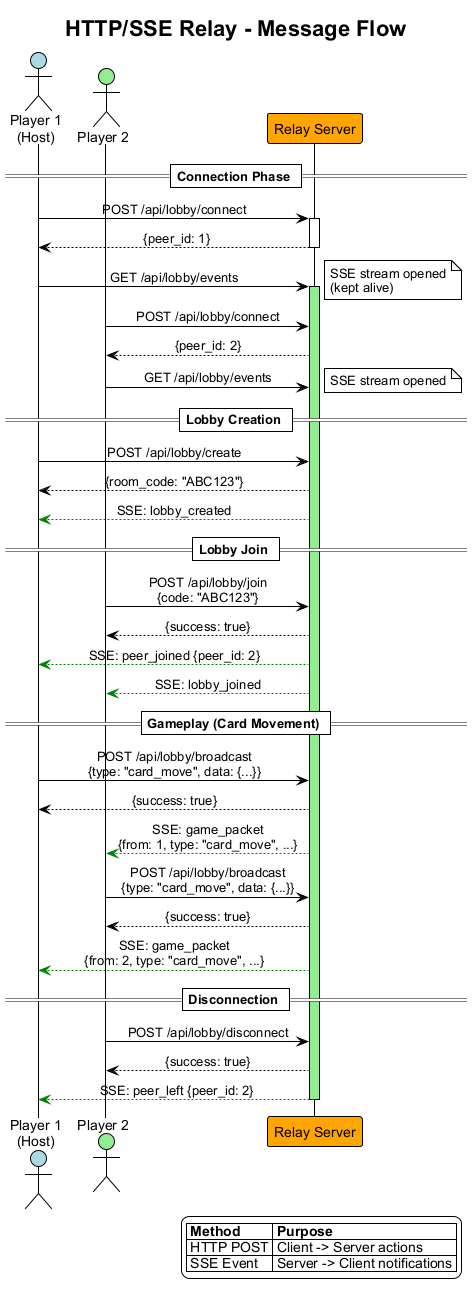
\includegraphics[width=0.75\textwidth]{figures/diagrams/http-sse-sequence.png}
    \caption{HTTP/SSE relay message flow: connection, lobby creation, and gameplay synchronization}
    \label{fig:http-sse-sequence}
\end{figure}

%-----------------------------------------------------------------------
\subsection{Supporting Development Toolchain}
\label{subsec:supporting-toolchain}

Beyond core engine/networking choices, several tools were selected to improve debugging observability, delivery speed, and reproducibility.

\begin{itemize}
    \item \textbf{ToastParty (Godot plugin)}: non-blocking UI event popups; improved usability feedback during multiplayer sessions \citep{toastparty_asset}.
    \item \textbf{VarTree (Godot plugin)}: runtime inspection/modification of sync variables; reduced debugging turnaround \citep{vartree_asset}.
    \item \textbf{Logger/custom logging client}: structured network/gameplay logs; improved diagnosis of timing and replication issues.
    \item \textbf{Python/aiohttp relay server}: browser-compatible signaling/relay backend for HTTP/SSE transport \citep{python_org,aiohttp_docs}.
    \item \textbf{Ruff}: linting and style checks for Python server/scripts; improved maintainability and consistency \citep{ruff_docs}.
    \item \textbf{justfile}: repeatable task automation for build/test/maintenance workflows \citep{just_docs}.
    \item \textbf{mkcert}: trusted local TLS certificates for secure browser multiplayer testing \citep{mkcert_repo}.
    \item \textbf{Chocolatey}: standardized Windows package setup, reducing environment variability \citep{chocolatey_platform}.
    \item \textbf{const\_generator}: generated constants to reduce manual duplication and config drift \citep{const_generator_asset}.
    \item \textbf{Git + GitHub}: version control, issue tracking, and collaborative documentation supporting reproducible research development \citep{git_scm,github_platform}.
\end{itemize}


%-----------------------------------------------------------------------
\subsection{Final Toolchain and Rationale Summary}
\label{subsec:toolchain-summary}

\begin{table}[htbp]
    \centering
    \caption{Final toolchain decisions and accepted trade-offs}
    \label{tab:toolchain-summary}
    \begin{tabular}{@{}p{2.8cm}p{2.6cm}p{4.5cm}p{4cm}@{}}
        \toprule
        \textbf{Tool}                & \textbf{Category}     & \textbf{Selected because}                        & \textbf{Trade-off accepted}                \\
        \midrule
        Godot 4.x                    & Engine                & Fast 2D/web workflow, open-source, small exports & Smaller ecosystem than Unity/Unreal        \\
        GDScript                     & Language              & Fast iteration and readability                   & Lower peak performance than C++            \\
        GDSync                       & Multiplayer framework & High-level synchronization abstractions          & Framework quirks and debugging overhead    \\
        HTTP/SSE relay (Python)      & Transport             & Browser compatibility and implementation control & Extra relay infrastructure and hop latency \\
        Supporting plugins/utilities & Toolchain             & Improved debugging, quality, and reproducibility & Additional maintenance surface             \\
        \bottomrule
    \end{tabular}
\end{table}

%-----------------------------------------------------------------------
\subsection{Development Approach}
\label{subsec:development-approach}

The game development followed an iterative, incremental approach spanning approximately 14~months (December~2024 to February~2026). Figure~\ref{fig:development-timeline} shows the five phases, key milestones, and decision pivots that shaped the architecture and tooling (see also Sections~\ref{subsec:tool-eval-process} and~\ref{subsec:toolchain-summary}; Chapter~\ref{ch:problems}, Section~\ref{subsec:web-patch-case-study}).

\begin{figure}[htbp]
    \centering
    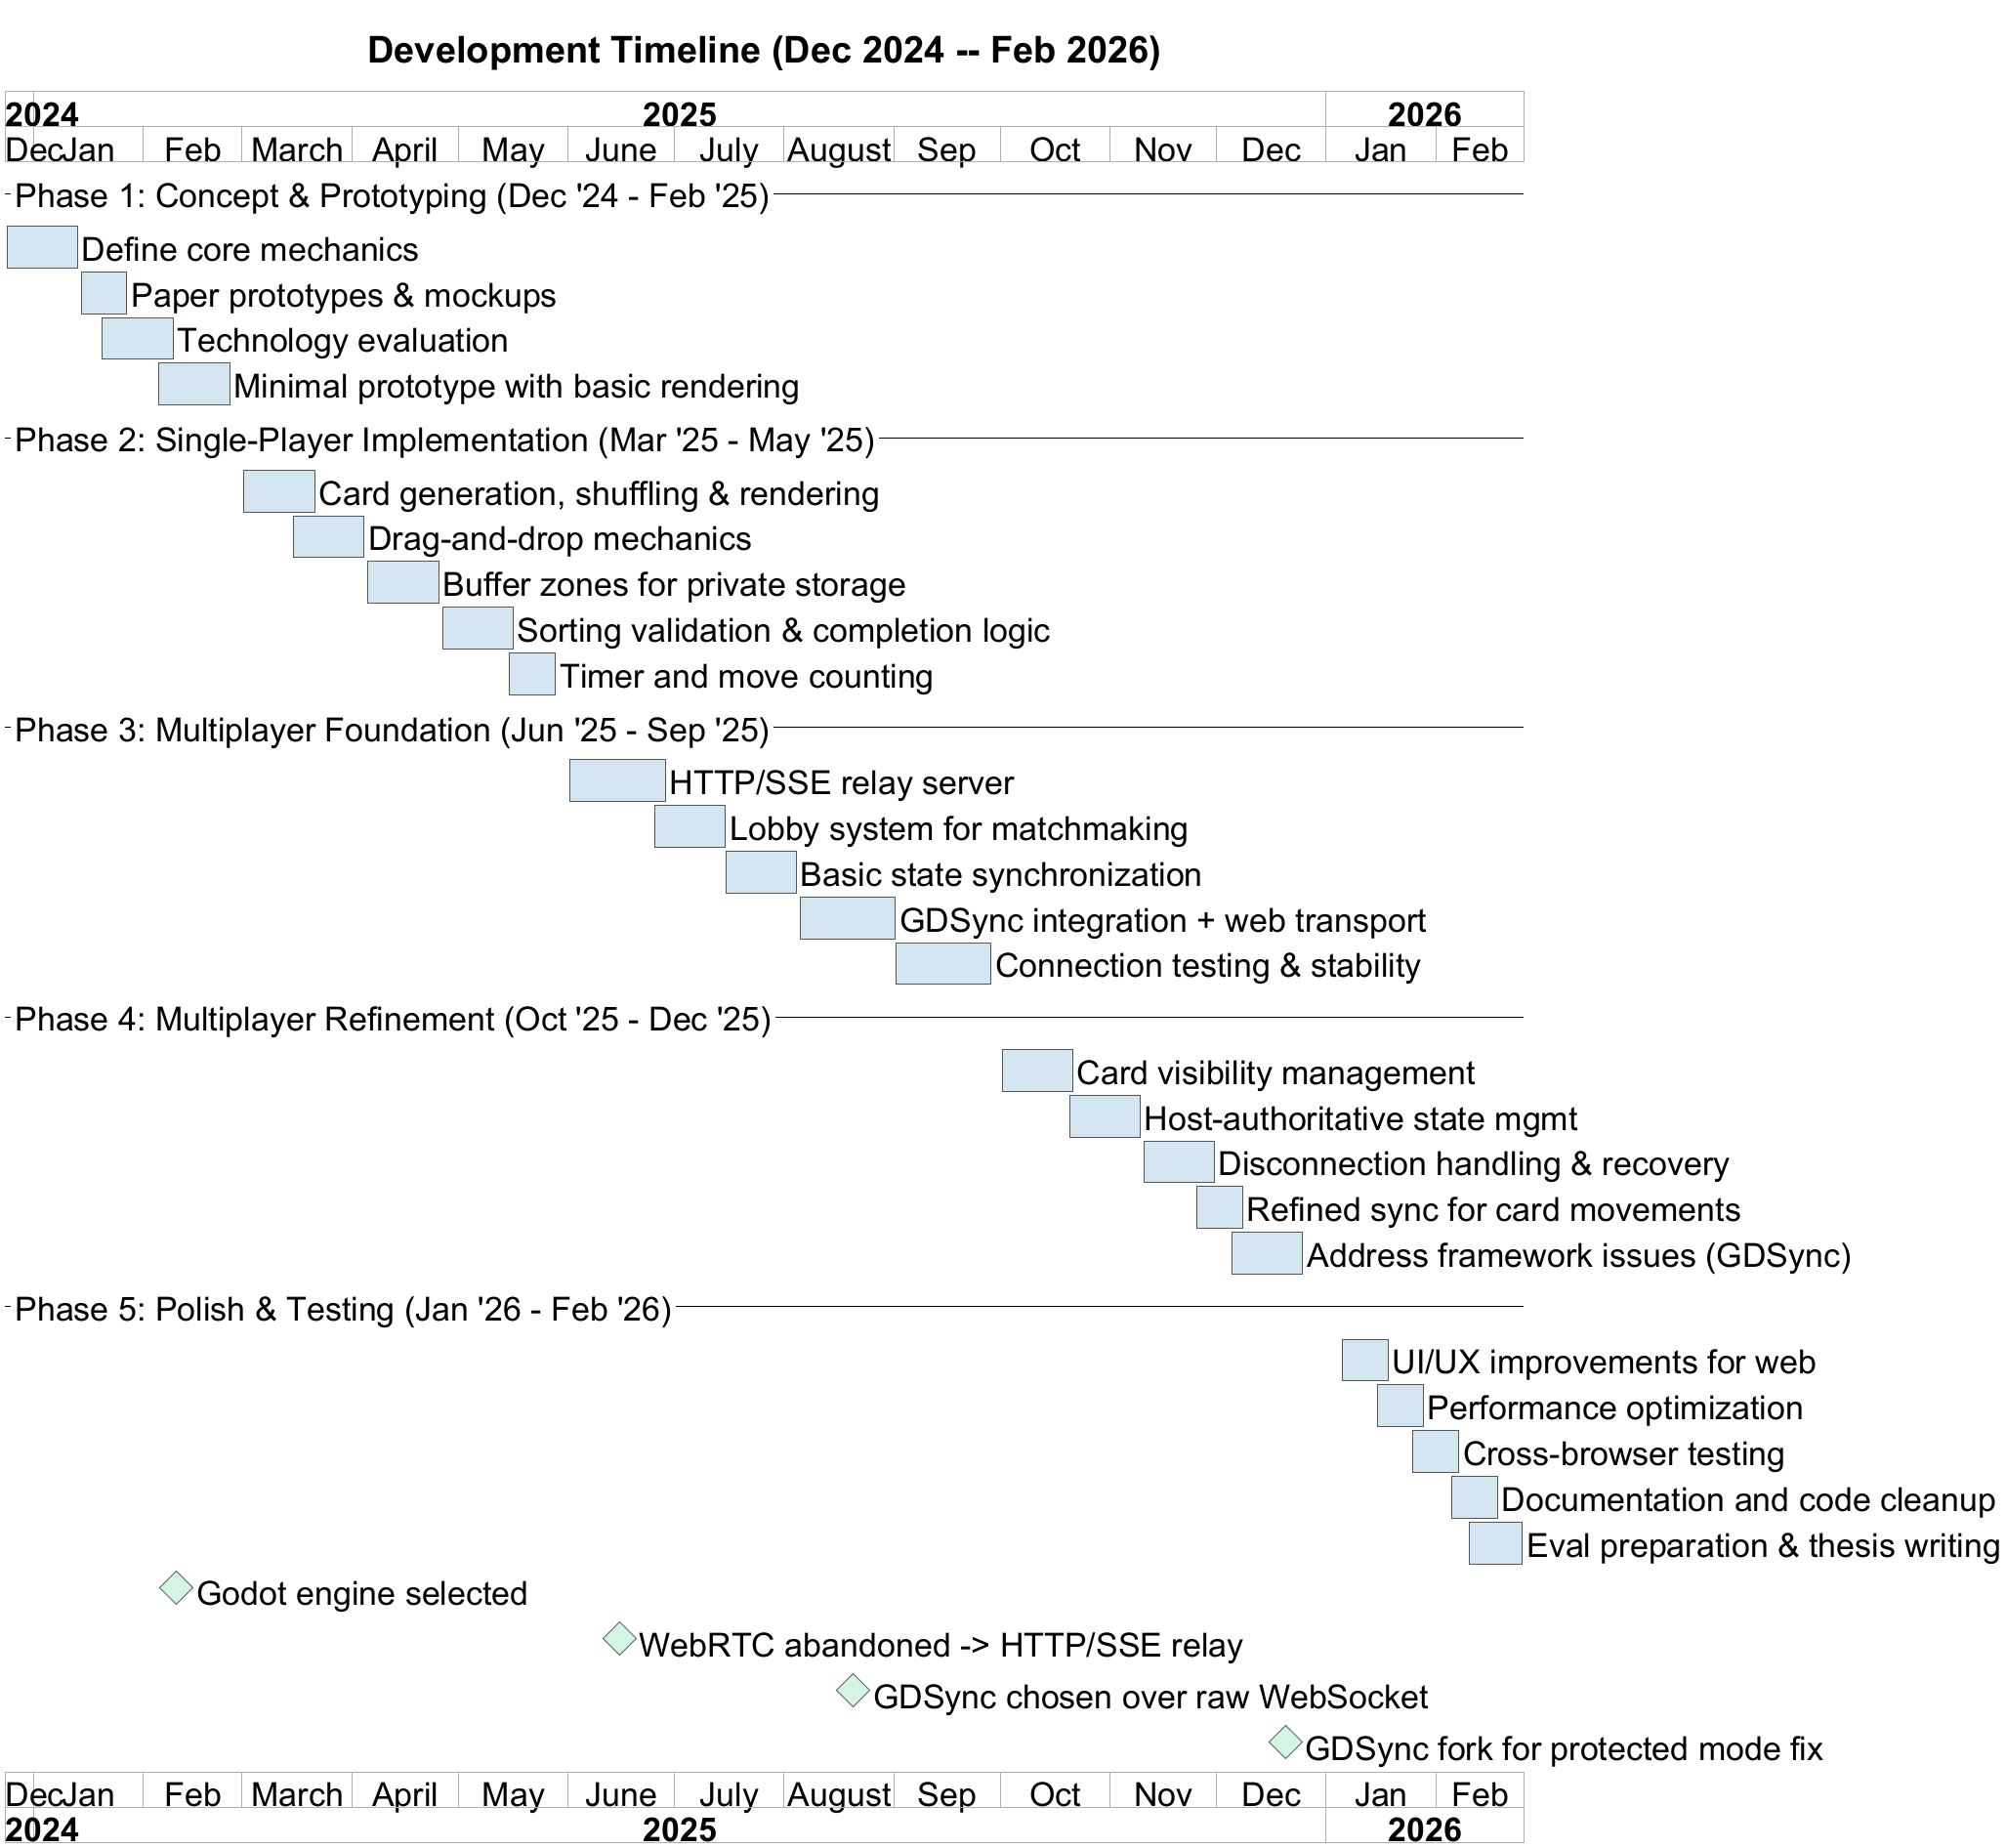
\includegraphics[width=\textwidth]{figures/diagrams/development-timeline-phases}
    \caption{Development timeline showing five project phases (December~2024 -- February~2026) with key decision pivots marked as milestones.}
    \label{fig:development-timeline}
\end{figure}

\paragraph*{Phase 1: Concept and Prototyping (December 2024 -- February 2025)}
\begin{itemize}
    \item Defined core mechanics based on physical card-sorting experiments
    \item Created paper prototypes and mockups
    \item Evaluated technology options (game engines, frameworks)
    \item Developed minimal prototype with basic card rendering
\end{itemize}

\paragraph*{Phase 2: Single-Player Implementation (March -- May 2025)}
\begin{itemize}
    \item Implemented card generation, shuffling, and rendering
    \item Developed drag-and-drop mechanics for touch and mouse input
    \item Created buffer zones for private card storage
    \item Implemented sorting validation and game completion logic
    \item Added timer and move counting
\end{itemize}

\paragraph*{Phase 3: Multiplayer Foundation (June -- September 2025)}
\begin{itemize}
    \item Developed HTTP/SSE relay server for web browser compatibility
    \item Implemented lobby system for matchmaking
    \item Developed basic state synchronization
    \item Integrated GDSync framework with custom web transport layer
    \item Tested connection establishment and stability
\end{itemize}

\paragraph*{Phase 4: Multiplayer Refinement (October -- December 2025)}
\begin{itemize}
    \item Implemented card visibility management (public buffers)
    \item Developed host-authoritative state management
    \item Added disconnection handling and recovery
    \item Refined synchronization for card movements
    \item Addressed framework issues (GDSync protected mode)
\end{itemize}

\paragraph*{Phase 5: Polish and Testing (January -- February 2026)}
\begin{itemize}
    \item UI/UX improvements for web usability
    \item Performance optimization (rendering, networking)
    \item Extensive testing across web browsers
    \item Documentation and code cleanup
    \item Preparation for evaluation and thesis writing
\end{itemize}

%-----------------------------------------------------------------------
\section{Game Design Methodology}
\label{sec:game-design}

%-----------------------------------------------------------------------
\subsection{Mapping HPC Concepts to Game Mechanics}
\label{subsec:concept-mapping}

The core challenge was translating abstract parallel computing concepts into tangible game mechanics. Table~\ref{tab:concept-mapping-methodology} shows the systematic mapping process:

\begin{table}[htbp]
    \centering
    \caption{Systematic mapping of HPC concepts to game mechanics}
    \label{tab:concept-mapping-methodology}
    \begin{tabular}{@{}p{3.5cm}p{4cm}p{5cm}@{}}
        \toprule
        \textbf{HPC Concept}   & \textbf{Real-World Analogy}        & \textbf{Game Mechanic}               \\
        \midrule
        Sequential Execution   & Single student working alone       & Single player in solo mode           \\
        \midrule
        Thread (OpenMP)        & Student with access to shared desk & Player in multiplayer mode           \\
        \midrule
        Shared Memory          & Desk visible to all students       & Shared card container                \\
        \midrule
        Per-Thread Work Area   & Student's section of a shared desk & Player's public buffer zones         \\
        \midrule
        Parallel Execution     & Students work simultaneously       & Multiple players, no turn-taking     \\
        \midrule
        Synchronization        & Students coordinate access         & Shared container access patterns     \\
        \midrule
        Memory Access Overhead & Time to reach shared desk          & Network latency to shared data       \\
        \midrule
        Speedup                & Multiple students finish faster    & Timer comparison: solo vs. multi     \\
        \midrule
        Load Balancing         & Even distribution of work          & Fair work distribution among players \\
        \bottomrule
    \end{tabular}
\end{table}

\paragraph*{Design Validation:}

The pedagogical mapping was validated through:
\begin{itemize}
    \item Comparison with Professor D'Agostino's physical experiments
    \item Review by HPC instructors for conceptual accuracy
    \item Pilot testing with students familiar with parallel computing
    \item Iterative refinement based on feedback
\end{itemize}

%-----------------------------------------------------------------------
\subsection{User Experience Design}
\label{subsec:ux-design}

\paragraph*{Design Principles:}

\begin{enumerate}
    \item \textbf{Minimize Cognitive Load}: Simple, clear visuals; avoid information overload
    \item \textbf{Immediate Feedback}: Every action produces visual/audio response
    \item \textbf{Progressive Disclosure}: Show information when needed, hide complexity initially
    \item \textbf{Error Prevention}: Design interface to prevent common mistakes
    \item \textbf{Aesthetic Simplicity}: Clean, uncluttered design focuses attention on cards
\end{enumerate}

\paragraph*{Interaction Design:}

Card interactions were designed to work with both touch and mouse input:

\begin{itemize}
    \item \textbf{Click/Tap to Select}: Quick click or tap selects a card (alternative to drag)
    \item \textbf{Drag to Move}: Click-and-hold initiates drag, release drops card
    \item \textbf{Scroll}: Vertical scroll moves through card container
    \item \textbf{Visual Feedback}: Cards scale up when dragged, drop zones highlight
\end{itemize}

\paragraph*{Color Coding:}

Colors convey semantic meaning:

\begin{itemize}
    \item \textbf{Blue}: Normal cards, main container
    \item \textbf{Yellow}: Highlighted cards during drag
    \item \textbf{Gray}: Disabled/hidden cards (other players' buffers)
    \item \textbf{Purple}: Player-specific UI elements (buffers, indicators)
\end{itemize}

%-----------------------------------------------------------------------
% Note: Difficulty progression (Easy/Medium/Hard modes) was not implemented
% in the current version. This is discussed as future work in Chapter 8.

%-----------------------------------------------------------------------
\section{Evaluation Methodology}
\label{sec:evaluation-methodology}

\subsection{Evaluation Criteria}
\label{subsec:evaluation-criteria}

The educational tool's success was evaluated across four primary dimensions:

\begin{enumerate}
    \item \textbf{Technical Performance}: Frame rate stability, memory consumption, and cross-browser compatibility.
    \item \textbf{Functional Completeness}: The successful implementation of all core required features.
    \item \textbf{Usability}: General ease of use, user learnability, and overall satisfaction.
    \item \textbf{Educational Effectiveness}: Indicators of user engagement and preliminary conceptual understanding (evaluated informally).
\end{enumerate}

\subsection{Evaluation Methods}
\label{subsec:evaluation-methods}

To assess the criteria outlined above, the following methodologies were applied:

\subsubsection*{Technical Benchmarking}
\begin{itemize}
    \item Performance profiling utilizing Godot's built-in diagnostic tools.
    \item Frame rate monitoring across target web browsers.
    \item Memory usage tracking during extended gameplay sessions.
\end{itemize}

\subsubsection*{Usability Testing}
\begin{itemize}
    \item Think-aloud protocols conducted with test users.
    \item Direct observation of first-time players interacting with the system.
    \item Measurement of task completion rates and completion times.
    \item Administration of the System Usability Scale (SUS) questionnaire to quantify user satisfaction. % Remove this line if you didn't actually do the SUS!
\end{itemize}

\subsubsection*{Educational Assessment}
\begin{itemize}
    \item Pre- and post-test knowledge assessments to measure conceptual growth. % Remove if you didn't do this!
    \item Concept mapping to evaluate the formation of parallel computing mental models.
    \item Qualitative feedback gathering regarding the perceived learning value of the serious game.
\end{itemize}

%-----------------------------------------------------------------------
\section{Development Tools and Environment}
\label{sec:dev-environment}

\paragraph*{Development Platform:}
\begin{itemize}
    \item \textbf{OS}: Windows 11 / Linux (Ubuntu 22.04)
    \item \textbf{IDE}: Visual Studio Code with GDScript extension
    \item \textbf{Engine}: Godot Engine 4.5.x
    \item \textbf{Version Control}: Git with GitHub repository
\end{itemize}

\paragraph*{Testing Environment:}
\begin{itemize}
    \item Primary: Chrome 120+ (Windows, macOS)
    \item Secondary: Firefox 120+ (Windows, Linux)
    \item Tertiary: Safari 17+ (macOS)
    \item Local development server for testing
\end{itemize}

\paragraph*{Build and Deployment:}
\begin{itemize}
    \item Web export (HTML5) built via Godot export templates
    \item Debug builds for development testing
    \item Release builds with optimizations for distribution
    \item Static file hosting for deployment
\end{itemize}

%-----------------------------------------------------------------------
\section{Summary}
\label{sec:methodology-summary}

This chapter described the comprehensive methodology employed to develop the HPC Sorting Serious Game:

\begin{itemize}
    \item \textbf{Research Approach}: Design Science Research framework with iterative development
    \item \textbf{Requirements}: Educational and functional requirements derived from learning objectives
    \item \textbf{Technology Selection}: Justified choices of Godot Engine, GDScript, GDSync, and HTTP/SSE relay architecture based on project needs
    \item \textbf{Game Design}: Systematic mapping of HPC concepts to game mechanics with UX design principles
    \item \textbf{Evaluation}: Multi-faceted evaluation approach combining technical, usability, and educational assessment
\end{itemize}

The next chapter presents the detailed system architecture resulting from these methodological decisions, including scene structure, component design, and multiplayer networking architecture.

% !TeX root = ../main.tex
\chapter{System Design and Architecture}
\label{ch:architecture}

This chapter presents the system architecture decisions that enabled the HPC Sorting Serious Game to be feasible, maintainable, and pedagogically interpretable. It focuses on architectural structure and rationale rather than exhaustive implementation listings. Detailed implementation is provided in Chapter~\ref{ch:implementation}, and educational/operational effectiveness is evaluated in Chapter~\ref{ch:results}.

%-----------------------------------------------------------------------
\section{Architectural Overview}
\label{sec:architectural-overview}

The architecture is organized to support two complementary goals:
\begin{itemize}
    \item \textbf{Pedagogical clarity}: game mechanics must remain interpretable as OpenMP-inspired shared-memory collaboration.
    \item \textbf{Technical robustness}: multiplayer synchronization must remain consistent across browser clients under variable latency.
\end{itemize}

%-----------------------------------------------------------------------
\subsection{Design Principles}
\label{subsec:design-principles}

The architecture is guided by the following principles:
\begin{enumerate}
    \item \textbf{Component modularity}: cards, buffers, and managers are separated so mechanics can evolve without rewriting the whole system.
    \item \textbf{Separation of concerns}: UI, game rules, and synchronization logic are isolated to reduce coupling during iterative experiments.
    \item \textbf{Host-authoritative conflict handling}: one authority resolves contested actions to prevent divergent multiplayer states.
    \item \textbf{Observable synchronization}: architecture includes explicit state transitions that can be logged and inspected during debugging.
    \item \textbf{Web-first constraints}: transport, update cadence, and payload design prioritize browser compatibility over engine-native networking assumptions.
\end{enumerate}

%-----------------------------------------------------------------------
\subsection{System Layers}
\label{subsec:system-layers}

\begin{description}
    \item[Presentation Layer] Renders cards, buffers, indicators, and interaction feedback.
    \item[Game Logic Layer] Validates sorting actions, completion conditions, and per-mode rules.
    \item[Synchronization Layer] Coordinates shared/private state propagation, ordering, and conflict resolution.
    \item[Transport/Relay Layer] Handles browser-compatible signaling and event relay via HTTP/SSE.
\end{description}

These layers decouple pedagogical behavior from transport mechanics, which was essential when adapting multiplayer behavior for browser export.

%-----------------------------------------------------------------------
\section{Scene and Interaction Architecture}
\label{sec:scene-structure}

The scene model is intentionally concise: a menu/lobby entry path and two gameplay contexts (single-player baseline and multiplayer OpenMP-style collaboration). The scene split supports direct comparison between sequential and collaborative execution while reusing core card and validation logic.
% TODO: [Artifact] Consolidated scene-transition/state diagram.
% TODO: [Purpose] Explain lifecycle transitions and their pedagogical meaning.
% TODO: [Source Inputs] scene_manager.gd; scenes/MainMenuScene/menu_scene.tscn; scenes/Multiplayer/Lobby/multiplayer_lobby.gd.
% TODO: [Placement] In this section, immediately after the "Architectural Intent" bullets.
% TODO: [Done Criteria] Include paths MainMenu -> SinglePlayer, MainMenu -> Lobby -> MultiplayerGame, and Gameplay -> Completion; each arrow must state trigger and learning implication.
% TODO: [Cross-refs] Chapter~\ref{ch:results}, Section~\ref{subsec:use-cases}.

\paragraph*{Architectural Intent:}
\begin{itemize}
    \item Single-player provides the sequential baseline for speedup interpretation.
    \item Multiplayer preserves shared container semantics while enforcing private buffer visibility.
    \item Lobby separates session orchestration from gameplay state transitions.
\end{itemize}

This scene structure keeps learning signals (who can see what, who can move what, when state is final) explicit for both users and evaluators.

%-----------------------------------------------------------------------
\subsection{Scene Lifecycle and Transition Logic}
\label{subsec:scene-lifecycle}

Scene changes are managed through a central scene manager to avoid ad-hoc transitions across gameplay scripts. This keeps navigation behavior deterministic and makes it easier to relate transitions to teaching intent (e.g., sequential baseline first, then collaborative mode).

%-----------------------------------------------------------------------
\subsection{Event-Driven Coordination}
\label{subsec:event-driven-architecture}

The architecture is event-driven at component boundaries. Local game objects communicate via Godot signals, while multiplayer state changes are propagated through authority-managed synchronization paths. This split allows UI responsiveness without directly coupling UI events to transport internals.
% TODO: [Artifact] Signal-flow map for one local interaction path and one multiplayer path.
% TODO: [Purpose] Show emitter/listener relationships and where authority checks occur.
% TODO: [Source Inputs] scenes/CardScene/scripts/card_manager.gd; scenes/Multiplayer/connection_manager.gd; scenes/Multiplayer/Lobby/multiplayer_lobby.gd.
% TODO: [Placement] End of this subsection, before Section~\ref{sec:core-components}.
% TODO: [Done Criteria] Include at least one local signal path and one connection/lobby event path with explicit event names.
% TODO: [Cross-refs] Section~\ref{subsec:connection-management}; Chapter~\ref{ch:implementation}, Section~\ref{subsec:lobby-system}.

%-----------------------------------------------------------------------
\section{Core Component Roles}
\label{sec:core-components}

Rather than duplicating full class implementations, this section summarizes architecture-critical component responsibilities.
% TODO: [Artifact] Compact UML/component-inheritance diagram.
% TODO: [Purpose] Document reusability-oriented class boundaries and extension points.
% TODO: [Source Inputs] scenes/CardScene/scripts/card_manager.gd; scenes/Multiplayer/MultiplayerGame/multiplayer_card_manager.gd.
% TODO: [Placement] After the Multiplayer Card Manager paragraph.
% TODO: [Done Criteria] Show CardManager -> MultiplayerCardManager inheritance and manager responsibility split.
% TODO: [Cross-refs] Chapter~\ref{ch:implementation}, Section~\ref{sec:impl-core-components}.

\paragraph*{Card Component (Interaction Unit):}
\label{subsec:card-component}
\begin{itemize}
    \item Encapsulates value identity, interaction state, and visual feedback states.
    \item Emits events consumed by manager-level logic rather than mutating global state directly.
\end{itemize}

\paragraph*{Card Manager (Rule and State Coordinator):}
\label{subsec:card-manager}
\begin{itemize}
    \item Owns sorting validity checks and authoritative placement updates.
    \item Serves as the integration boundary between UI interaction and synchronization rules.
    \item Was designed for reusability: shared logic lives in \texttt{card\_manager.gd} so mode-specific behavior can be layered instead of duplicated.
\end{itemize}

\paragraph*{Multiplayer Card Manager (Authority Extension):}
\label{subsec:multiplayer-card-manager}
\begin{itemize}
    \item Explicitly extends \texttt{card\_manager.gd} as \texttt{multiplayer\_card\_manager.gd}, adding host-authoritative synchronization and reconciliation behavior while reusing baseline card/rule logic.
    \item Enforces shared/private visibility semantics across peers.
\end{itemize}

%-----------------------------------------------------------------------
\section{Multiplayer Architecture}
\label{sec:multiplayer-architecture}

%-----------------------------------------------------------------------
\subsection{Network Topology}
\label{subsec:network-topology}

The implemented multiplayer topology uses browser-compatible relay patterns for session events and state updates. This avoids assumptions that are unstable in browser-exported runtime contexts.
% TODO: [Artifact] Deployment/context diagram with authority boundaries.
% TODO: [Purpose] Distinguish in-process signal communication from inter-client relay communication.
% TODO: [Source Inputs] figures/diagrams/http-sse-architecture.png; scenes/Multiplayer/connection_manager.gd; scenes/Multiplayer/GDSyncWebPatch/local_server_signaling.gd.
% TODO: [Placement] Near Figure~\ref{fig:http-sse-architecture}, as a companion context figure.
% TODO: [Done Criteria] Show browser clients, signaling/relay server, host authority decision point, and shared/private state propagation boundary.
% TODO: [Cross-refs] Chapter~\ref{ch:problems}, Section~\ref{subsec:web-patch-case-study}.

\begin{figure}[htbp]
    \centering
    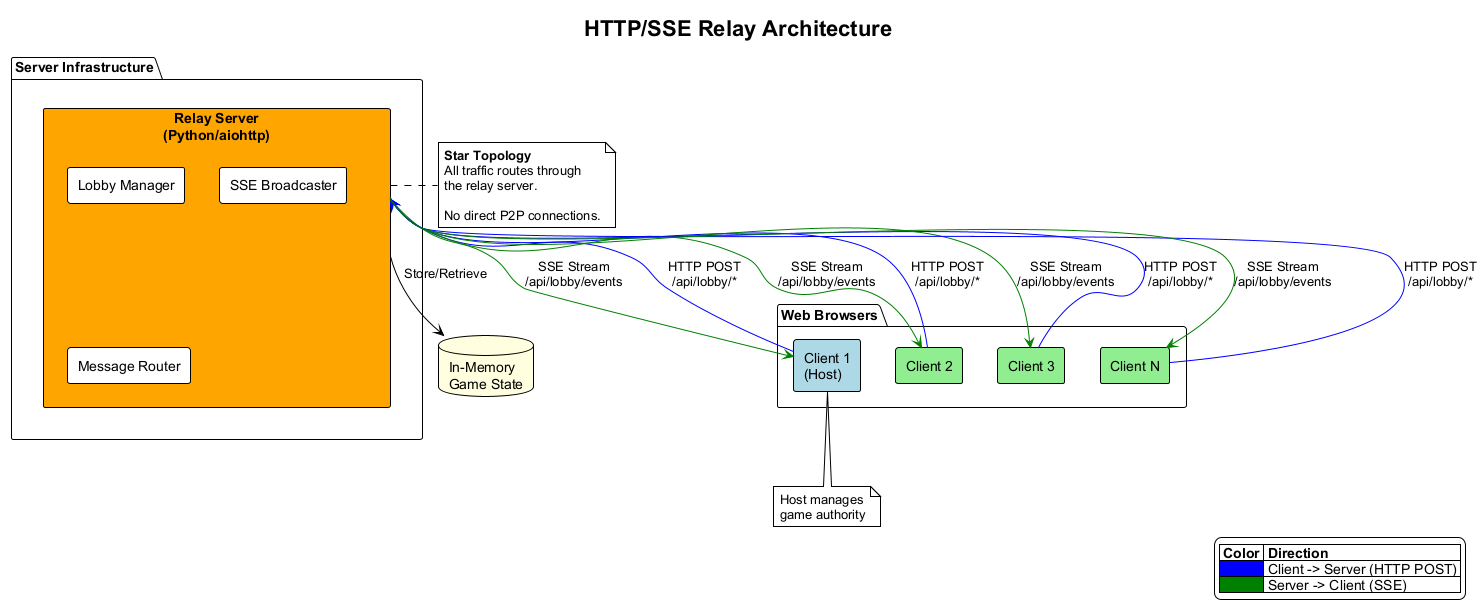
\includegraphics[width=0.82\textwidth]{figures/diagrams/http-sse-architecture.png}
    \caption{HTTP/SSE relay-oriented architecture used for web-first multiplayer synchronization}
    \label{fig:http-sse-architecture}
\end{figure}

%-----------------------------------------------------------------------
\subsection{State Synchronization Patterns}
\label{subsec:state-sync-patterns}

Two synchronization patterns are central:
\begin{itemize}
    \item \textbf{Optimistic local interaction}: local responsiveness is preserved while awaiting authoritative confirmation.
    \item \textbf{Host broadcast reconciliation}: final shared state is re-broadcast to all peers to converge state.
\end{itemize}

\begin{lstlisting}[language=Python, caption={Architectural pattern: host-authoritative move confirmation}]
# Client proposes move -> host validates -> host broadcasts canonical state
on_client_move(card_id, target_slot):
    if host_validate(card_id, target_slot):
        host_apply(card_id, target_slot)
        broadcast_canonical_state(card_id, target_slot)
    else:
        reject_and_restore(card_id)
\end{lstlisting}

This pattern minimizes permanent divergence while preserving interaction fluidity.

%-----------------------------------------------------------------------
\subsection{GDSync Integration Boundary}
\label{subsec:gdsync-integration}

GDSync is treated as a synchronization abstraction layer, while architecture ownership remains in the game managers. This prevented framework-specific behavior from leaking into all gameplay components and reduced replacement cost when debugging framework limitations.
The web-export signaling patch details are intentionally analyzed in Chapter~\ref{ch:problems}, Section~\ref{subsec:web-patch-case-study}, while this section keeps the architectural boundary view.
% TODO: [Artifact] Real (non-pseudocode) manager-boundary code excerpt.
% TODO: [Purpose] Prove the wrapper/delegation boundary and authority checkpoint in actual project code.
% TODO: [Source Inputs] scenes/Multiplayer/MultiplayerGame/multiplayer_card_manager.gd; scenes/Multiplayer/connection_manager.gd.
% TODO: [Placement] Replace the pseudocode listing or place immediately below it.
% TODO: [Done Criteria] Excerpt shows sync entrypoint delegating into manager logic and where authority is enforced.
% TODO: [Cross-refs] Chapter~\ref{ch:problems}, Section~\ref{subsec:web-patch-case-study}.

\begin{lstlisting}[language=Python, caption={Architectural boundary: sync wrapper delegates to game manager}]
@GDSync.rpc(call_local=true)
func sync_move(card_id: int, target_id: int):
    multiplayer_manager.apply_authoritative_move(card_id, target_id)
\end{lstlisting}

%-----------------------------------------------------------------------
\subsection{Connection Management}
\label{subsec:connection-management}

Connection handling is split into phases:
\begin{itemize}
    \item \textbf{Lobby phase}: peer discovery, readiness, and session configuration.
    \item \textbf{Gameplay phase}: synchronized interaction and reconciliation.
    \item \textbf{Failure phase}: disconnection detection and graceful degradation.
\end{itemize}

%-----------------------------------------------------------------------
\section{Data Flow and Visibility Model}
\label{sec:data-flow}

The architecture explicitly distinguishes:
\begin{itemize}
    \item \textbf{Shared-visible state}: container cards and game-level counters.
    \item \textbf{Player-private state}: cards in private buffers hidden from other players.
\end{itemize}

This model is central to the OpenMP analogy: all participants can access shared memory, while local buffer state remains private.
% TODO: [Artifact] Card-move sequence/data-flow diagram.
% TODO: [Purpose] Show end-to-end state transition from user action to converged visibility state.
% TODO: [Source Inputs] scenes/Multiplayer/MultiplayerGame/multiplayer_card_manager.gd; scenes/CardScene/scripts/card_manager.gd.
% TODO: [Placement] Directly after this paragraph and before the visibility listing.
% TODO: [Done Criteria] Must include propose -> validate -> authoritative apply -> broadcast -> visibility-gate update and identify shared vs private divergence points.
% TODO: [Cross-refs] Section~\ref{subsec:state-sync-patterns}; Chapter~\ref{ch:results}, Section~\ref{subsec:learner-messages}.

\begin{lstlisting}[language=Python, caption={Architectural mechanism: private buffer visibility gate}]
if card.in_private_buffer():
    card.visible = (card.buffer_owner_id == local_player_id)
else:
    card.visible = true
\end{lstlisting}

%-----------------------------------------------------------------------
\section{Barrier Synchronization Architecture}
\label{sec:barrier-architecture}

The game includes a barrier synchronization feature that directly models the \texttt{\#pragma omp barrier} construct from OpenMP. Architecturally, the barrier is implemented as a separate \texttt{BarrierManager} component (not embedded in the card manager) following the single-responsibility principle.

\subsection{State Machine Design}
\label{subsec:barrier-state-design}

The barrier operates as a three-state finite automaton with the following transitions:

\begin{enumerate}
    \item \textbf{RUNNING} $\to$ \textbf{WAITING\_AT\_BARRIER}: Any player initiates a barrier; all must arrive.
    \item \textbf{WAITING\_AT\_BARRIER} $\to$ \textbf{BARRIER\_ACTIVE}: All players have reached the barrier; the main thread is granted exclusive access to the shared container.
    \item \textbf{BARRIER\_ACTIVE} $\to$ \textbf{RUNNING}: The main thread releases the barrier; normal play resumes.
\end{enumerate}

This maps directly to OpenMP barrier semantics: threads reaching the barrier must wait until all threads have arrived, after which execution proceeds in a coordinated fashion.

\subsection{Integration Points}
\label{subsec:barrier-integration}

The \texttt{BarrierManager} integrates with the multiplayer card manager through three mechanisms:
\begin{itemize}
    \item \textbf{Signals}: emits \texttt{barrier\_state\_changed} to trigger UI overlays (lock screen for non-main-thread players).
    \item \textbf{GDSync exposure}: barrier functions are registered for remote invocation alongside card synchronization functions.
    \item \textbf{Settings}: BarrierManager reads the barrier mode (first-to-reach or round-robin) from the global \texttt{Settings} autoload.
\end{itemize}

\noindent The barrier implementation details are covered in Chapter~\ref{ch:implementation}, Section~\ref{sec:barrier-implementation}.

%-----------------------------------------------------------------------
\section{Responsive UI/UX Architecture}
\label{sec:responsive-ui-ux}

UI architecture prioritizes interpretable interaction under constrained viewports:
\begin{itemize}
    \item Scrollable container strategy for large card sets.
    \item Buffer-first layout to reinforce shared/private distinction.
    \item Immediate feedback (toast/status indicators) to reduce action ambiguity in multiplayer.
\end{itemize}

%-----------------------------------------------------------------------
\subsection{UI Layering and Overlay Isolation}
\label{subsec:ui-layering}

Overlay and inspection elements are separated from gameplay nodes to minimize accidental coupling between debug/auxiliary UI and gameplay transforms. This layering approach supports live inspection tooling while preserving gameplay interaction consistency.
% TODO: [Artifact] Node-tree snapshot and short explanatory caption for UI layering.
% TODO: [Purpose] Clarify why CanvasLayer-based overlays do not interfere with gameplay-space nodes.
% TODO: [Source Inputs] scenes/MainMenuScene/menu_scene.tscn (CanvasLayer, VarTreeMainMenu).
% TODO: [Placement] In this subsection as a compact figure or annotated listing.
% TODO: [Done Criteria] Clearly shows gameplay nodes vs overlay/debug nodes and the isolation rationale.
% TODO: [Cross-refs] Chapter~\ref{ch:implementation}, Section~\ref{subsec:vartree}.

A playful evasive hover animation is also present in the main menu as a non-critical engagement microinteraction; its reception in early tests is discussed in Chapter~\ref{ch:results}, Section~\ref{subsec:engagement-effects}.

%-----------------------------------------------------------------------
\section{Performance and Scalability Constraints}
\label{sec:performance}

Architecture-level performance strategies include:
\begin{itemize}
    \item bounded synchronization payloads,
    \item authoritative reconciliation instead of full scene replication,
    \item UI/container policies that remain usable at higher card counts.
\end{itemize}

Observed constraints and measured outcomes are discussed in Chapter~\ref{ch:results}.

%-----------------------------------------------------------------------
\section{Summary}
\label{sec:architecture-summary}

This chapter documented architectural decisions that made the tool technically feasible and pedagogically interpretable in a web-first multiplayer context. The focus was on synchronization boundaries, state visibility semantics, and authority patterns rather than exhaustive implementation detail. Detailed implementation evidence is provided in Chapter~\ref{ch:implementation}, while educational and operational effectiveness is evaluated in Chapter~\ref{ch:results}.

% !TeX root = ../main.tex
\chapter{Implementation}
\label{ch:implementation}

This chapter presents key implementation mechanisms of the HPC Sorting Serious Game. It covers the core game logic, multiplayer synchronization protocol, barrier synchronization (a direct pedagogical mapping to \texttt{\#pragma omp barrier}), the web-export compatibility patch, and development observability tooling. Tool/framework selection rationale is documented in Chapter~\ref{ch:methodology}, architectural decisions in Chapter~\ref{ch:architecture}, and effectiveness evaluation in Chapter~\ref{ch:results}.

The complete source code is available in the project repository \citep{github_project}. External tool and framework links are listed in Appendix~\ref{app:d:tool-links}.

%-----------------------------------------------------------------------
\section{Implementation Focus Areas}
\label{sec:impl-core-components}

The implementation evidence is organized around six high-impact concerns:
\begin{itemize}
    \item card management and sorting correctness,
    \item component reuse through inheritance (\texttt{CardManager} $\to$ \texttt{MultiplayerCardManager}),
    \item network state serialization and synchronization protocol,
    \item barrier synchronization as a pedagogical feature,
    \item web-export compatibility patching,
    \item observability and debuggability for multiplayer faults.
\end{itemize}

%-----------------------------------------------------------------------
\section{Card Management and Sorting Correctness}
\label{sec:singleplayer-implementation}

The single-player card management logic resides in \texttt{card\_manager.gd} (705~lines), which serves as both the standalone game controller and the base class for multiplayer extension.

%-----------------------------------------------------------------------
\subsection{Card Generation and Initialization}
\label{subsec:card-generation}

Card generation supports configurable counts (10--200) with optional unique or repeated values. The initialization sequence in \texttt{\_ready()} follows a deterministic pipeline:

\begin{lstlisting}[caption={Card manager initialization pipeline (card\_manager.gd)}]
func _ready():
    if num_cards < 1:
        num_cards = 1
    values = generate_random_values()
    sorted_all = values.duplicate()
    sorted_all.sort()

    adjust_container_spacing()
    cards_array = generate_completed_card_array(values)
    sorted_cards_array = generate_completed_card_array(sorted_all, "SortedCard_")
    fill_card_container(cards_array, card_container)
    fill_card_container(sorted_cards_array, sorted_cards_container)
    slots = create_buffer_slots()
    _connect_signals()
\end{lstlisting}

Each card is instantiated from a preloaded scene, assigned a numeric value and a color derived from the value (for visual distinctiveness), and placed in a scrollable \texttt{HBoxContainer}. A parallel sorted reference array is generated so players can optionally view the target ordering.

%-----------------------------------------------------------------------
\subsection{Sorting Validation}
\label{subsec:sorting-validation}

Sorting validation is the completion contract used in both single-player and multiplayer modes. The actual implementation iterates over the card container's children (the authoritative UI ordering):

\begin{lstlisting}[caption={Sorting validation (card\_manager.gd, line 645)}]
func check_sorting_order() -> bool:
    var sorted_correctly = true
    if card_container.get_child_count() != num_cards:
        return false
    var cards_in_container: Array[Card] = []
    for child in card_container.get_children():
        if child is Card:
            cards_in_container.append(child as Card)
    for i in range(1, cards_in_container.size()):
        var current_card = cards_in_container[i].value
        var previous_card = cards_in_container[i - 1].value
        if current_card < previous_card:
            sorted_correctly = false
            break
    return sorted_correctly
\end{lstlisting}

This mechanism provides a deterministic completion criterion independent of UI animation state and network timing. Notably, validation checks the \emph{scene tree child order} rather than an abstract array, ensuring that what the player sees matches what is validated (see Chapter~\ref{ch:results}, Section~\ref{sec:requirements-comparison}).

%-----------------------------------------------------------------------
\subsection{Buffer Contiguity Check}
\label{subsec:buffer-contiguity}

Players use private buffer zones (simulating thread-local storage) to temporarily hold cards during sorting. A buffer contiguity check validates that cards in the buffer form a contiguous subsequence of the sorted target:

\begin{lstlisting}[caption={Buffer contiguity validation (card\_manager.gd, line 693)}]
func check_player_buffer_contiguity() -> bool:
    var buffer_values = []
    for slot in slots:
        if slot.occupied_by == null:
            return false
        buffer_values.append(slot.occupied_by.value)
    return SubarrayUtils.is_contiguous_subarray(sorted_all, buffer_values)
\end{lstlisting}

This constraint reinforces the pedagogical mapping: just as a thread in an OpenMP program should work on a logically coherent subset of data, players must select contiguous card ranges for their buffers.

%-----------------------------------------------------------------------
\section{Component Reuse: CardManager Inheritance}
\label{sec:component-reuse}

The multiplayer game controller, \texttt{MultiplayerCardManager} (1143~lines), explicitly extends the single-player \texttt{CardManager}:

\begin{lstlisting}[caption={Multiplayer extension declaration (multiplayer\_card\_manager.gd, line 1)}]
extends "res://scenes/CardScene/scripts/card_manager.gd"
class_name MultiplayerCardManager
\end{lstlisting}

This inheritance structure allows the multiplayer mode to reuse all card generation, UI layout, sorting validation, and buffer management logic while adding:
\begin{itemize}
    \item host/client role differentiation,
    \item network state serialization (via \texttt{CardState}),
    \item GDSync function exposure for remote procedure calls,
    \item barrier synchronization integration.
\end{itemize}

The multiplayer \texttt{\_ready()} overrides the parent to branch on host vs.\ client role:

\begin{lstlisting}[caption={Multiplayer initialization with host/client branching (multiplayer\_card\_manager.gd)}]
func _ready():
    is_host = ConnectionManager.am_i_host()
    my_client_id = ConnectionManager.get_my_client_id()

    barrier_manager = BarrierManager.new()
    barrier_manager.set_barrier_mode(Settings.barrier_mode)
    barrier_manager.barrier_state_changed.connect(_on_barrier_state_changed)

    setup_multiplayer_sync()

    if is_host:
        super._ready()
        await get_tree().process_frame
        broadcast_initial_game_state()
        game_state_synced = true
    else:
        _initialize_client_structure()
        await get_tree().create_timer(0.5).timeout
        request_game_state_from_host()
\end{lstlisting}

The host executes the parent \texttt{\_ready()} (generating cards normally) and then broadcasts the initial state. Clients initialize an empty UI structure and request the authoritative game state from the host, avoiding duplicate card generation that would cause divergence.

%-----------------------------------------------------------------------
\section{Multiplayer Synchronization Protocol}
\label{sec:multiplayer-implementation}

%-----------------------------------------------------------------------
\subsection{CardState Serialization}
\label{subsec:cardstate-serialization}

All card state transmitted over the network is serialized through a dedicated \texttt{CardState} inner class:

\begin{lstlisting}[caption={CardState transport protocol (multiplayer\_card\_manager.gd, lines 6--49)}]
class CardState:
    var value: int
    var index: int
    var original_index: int
    var in_container: bool
    var in_buffer: bool
    var buffer_owner: int

    func to_dict() -> Dictionary:
        return {
            "value": value,
            "index": index,
            "original_index": original_index,
            "in_container": in_container,
            "in_buffer": in_buffer,
            "buffer_owner": buffer_owner
        }

    static func from_dict(data: Dictionary) -> CardState:
        return CardState.new(
            data.get("value", 0),
            data.get("index", -1),
            data.get("original_index", -1),
            data.get("in_container", true),
            data.get("in_buffer", false),
            data.get("buffer_owner", -1)
        )
\end{lstlisting}

\texttt{CardState} captures whether a card is in the shared container or in a player's private buffer, and who owns it. This explicit serialization boundary ensures that network payloads are minimal and self-describing, and that deserialization on the receiving client produces a deterministic scene state.

%-----------------------------------------------------------------------
\subsection{Lobby and Session Lifecycle}
\label{subsec:lobby-system}

The lobby manages session creation/joining and readiness transitions before gameplay authority is established.

\begin{enumerate}
    \item Player creates room or enters room code
    \item Connection to signaling server via HTTP/SSE
    \item Peer handshake with host
    \item Players appear in lobby list
    \item Host configures game settings (card count, buffer size, barrier mode)
    \item Host starts game, triggering scene transition to multiplayer gameplay
\end{enumerate}

\begin{figure}[htbp]
    \centering
    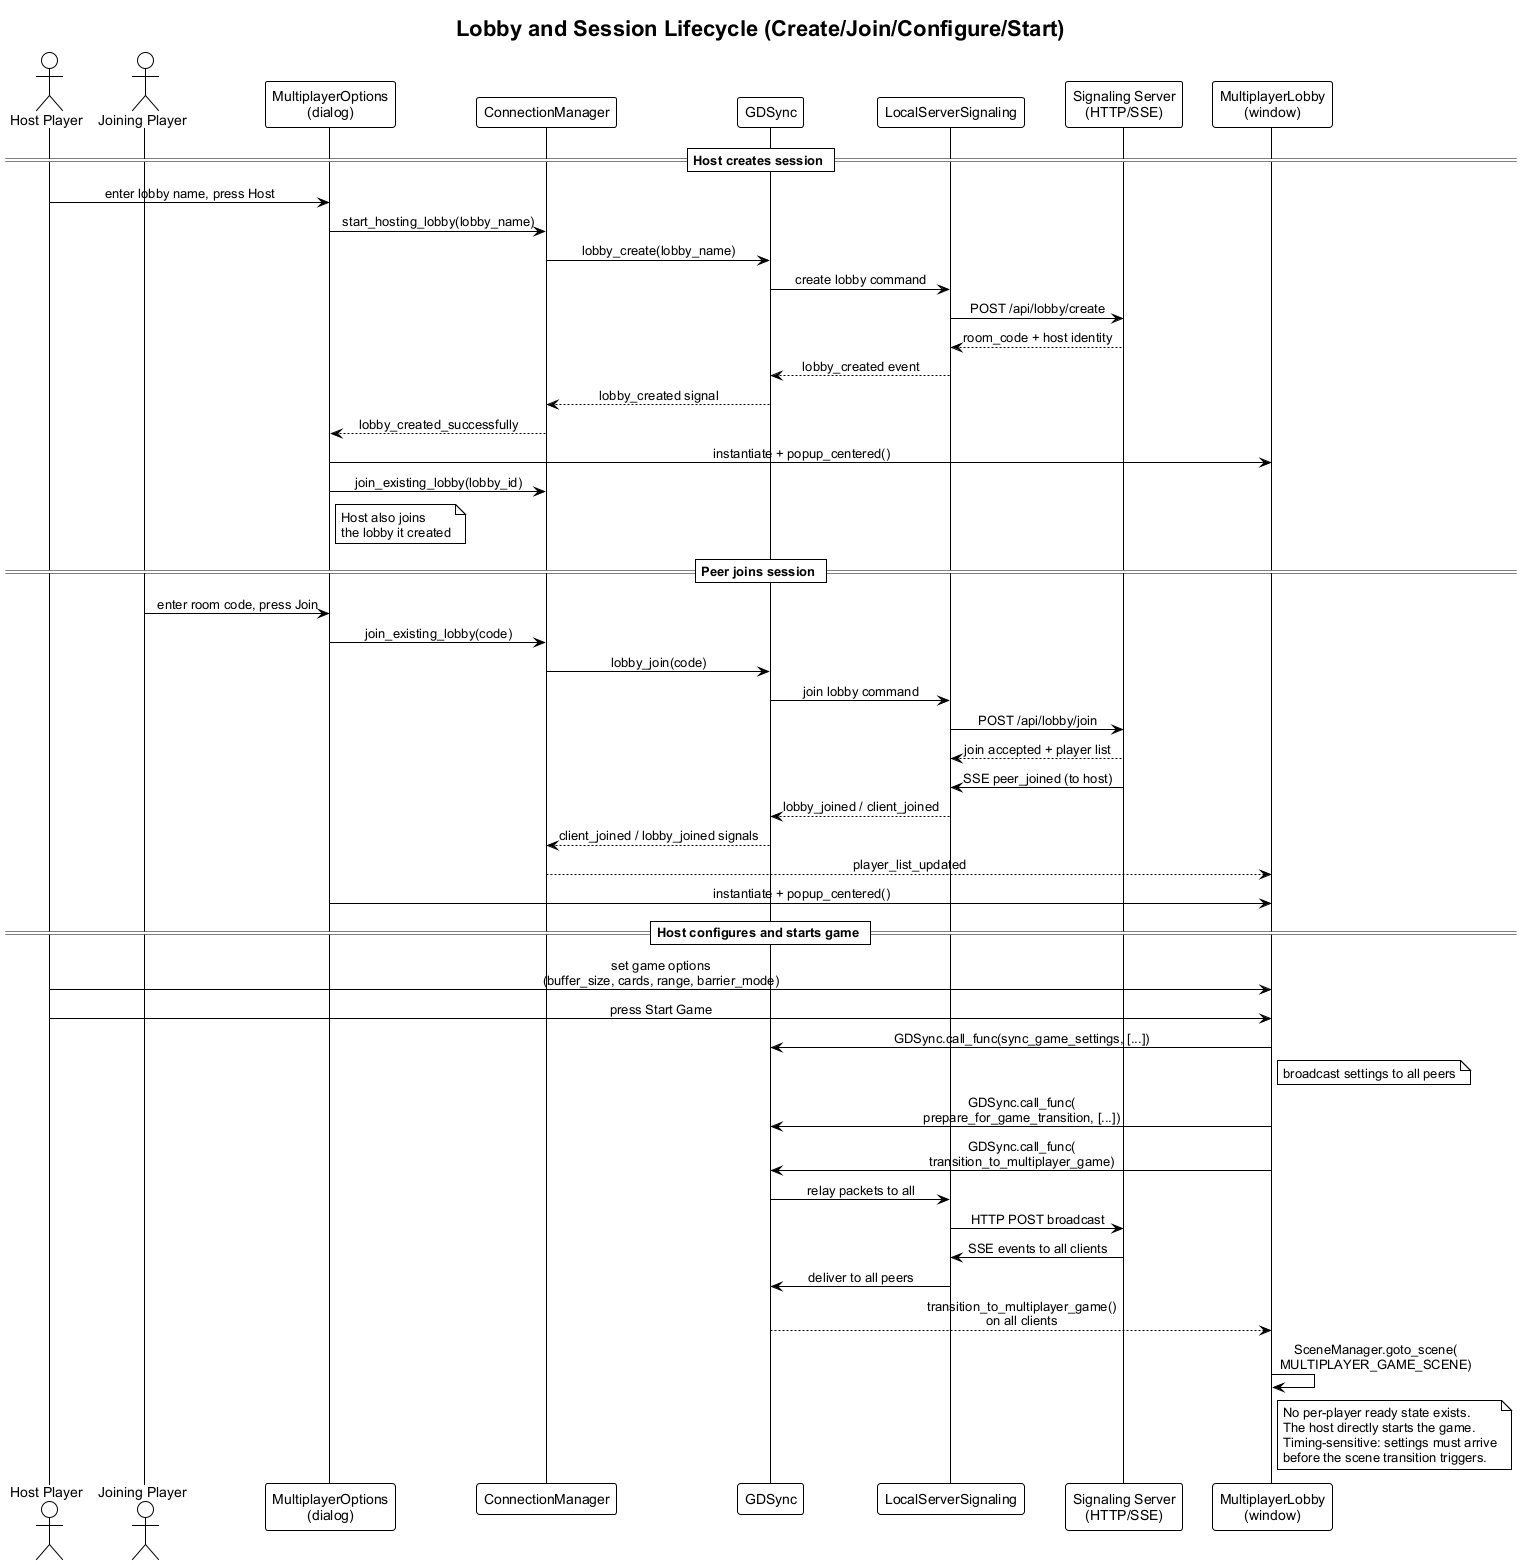
\includegraphics[width=0.92\textwidth]{figures/diagrams/lobby-session-lifecycle-sequence}
    \caption{Lobby and session lifecycle from room creation/join to synchronized game start}
    \label{fig:lobby-session-lifecycle-sequence}
\end{figure}

%-----------------------------------------------------------------------
\subsection{GDSync Function Exposure}
\label{subsec:impl-gdsync-integration}

GDSync provides high-level networking abstractions. For this thesis, the project uses an author-maintained GDSync fork that includes a fix required for the web-export workflow \citep{gdsync_fork}. A pull request with this fix was submitted upstream \citep{gdsync_framework}.

Rather than using decorator-based annotations, the actual GDSync integration uses explicit function exposure. The \texttt{setup\_multiplayer\_sync()} method registers all remotely callable functions:

\begin{lstlisting}[caption={GDSync function exposure (multiplayer\_card\_manager.gd)}]
func setup_multiplayer_sync():
    GDSync.expose_func(self.sync_complete_game_state)
    GDSync.expose_func(self.sync_card_moved)
    GDSync.expose_func(self.sync_card_entered_buffer)
    GDSync.expose_func(self.sync_card_left_buffer)
    GDSync.expose_func(self.sync_timer_state)
    GDSync.expose_func(self.sync_game_finished)
    GDSync.expose_func(self.send_current_state_to)
    # Barrier synchronization functions
    GDSync.expose_func(self.barrier_thread_reached)
    GDSync.expose_func(self.barrier_activate)
    GDSync.expose_func(self.barrier_card_picked)
    GDSync.expose_func(self.barrier_release)
\end{lstlisting}

Remote calls are then dispatched via \texttt{GDSync.call\_func()} (broadcast) or \texttt{GDSync.call\_func\_on()} (targeted to a specific peer). This explicit exposure model was required because GDSync's ``protected mode'' silently drops calls to unexposed functions (see Chapter~\ref{ch:problems}, Section~\ref{subsec:protected-mode-issue}).

%-----------------------------------------------------------------------
\subsection{State Broadcast and Reconciliation}
\label{subsec:state-broadcast}

When a card is placed in the main container (shared memory), the multiplayer manager overrides the parent handler to broadcast the move:

\begin{lstlisting}[caption={Card movement broadcast (multiplayer\_card\_manager.gd)}]
func _on_card_placed_in_container(
    dropped_card: Card = null,
    was_in_buffer: bool = false,
    original_slot: Variant = null
):
    super._on_card_placed_in_container()
    await get_tree().process_frame
    var new_index = moved_card.get_index()

    if was_in_buffer:
        GDSync.call_func(
            self.sync_card_left_buffer,
            [moved_card.value, my_client_id, new_index]
        )
    else:
        GDSync.call_func(
            self.sync_card_moved,
            [moved_card.value, moved_card.original_index,
             new_index, my_client_id]
        )
\end{lstlisting}

Clients receiving a \texttt{sync\_card\_moved} call skip the update if it originated from themselves (preventing echo loops), then reposition the card in their local scene tree:

\begin{lstlisting}[caption={Remote card movement handler (multiplayer\_card\_manager.gd)}]
func sync_card_moved(
    card_value: int, from_index: int, to_index: int, moving_client_id: int
):
    if moving_client_id == my_client_id:
        return
    var card: Card = _find_card_by_value(card_value)
    if not card:
        push_error("Card not found: ", card_value)
        return
    if card.get_parent() != card_container:
        if card.get_parent():
            card.get_parent().remove_child(card)
        card_container.add_child(card)
    card_container.move_child(card, to_index)
    card.visible = true
    card.set_can_drag(true)
\end{lstlisting}

%-----------------------------------------------------------------------
\subsection{Visibility Management}
\label{subsec:visibility-management}

In multiplayer mode (OpenMP simulation), players should not see cards in other players' private buffers, representing thread-private data. When a card enters another player's buffer, it is tracked locally and removed from the container:

\begin{lstlisting}[caption={Buffer entry notification (multiplayer\_card\_manager.gd)}]
func sync_card_entered_buffer(card_value: int, entering_player_id: int):
    if entering_player_id == my_client_id:
        return
    var card: Card = _find_card_by_value(card_value)
    if not card:
        return
    if card.get_parent() == card_container:
        card_container.remove_child(card)
    cards_in_other_buffers[card_value] = entering_player_id
\end{lstlisting}

Cards in \texttt{cards\_in\_other\_buffers} are invisible to the local player. When a card leaves another player's buffer, the reverse operation adds it back to the container. This mechanism preserves the shared-vs-private memory distinction that users report recognizing in evaluation sessions (Chapter~\ref{ch:results}, Sections~\ref{subsec:educational-features} and~\ref{subsec:learner-messages}).

%-----------------------------------------------------------------------
\section{Barrier Synchronization}
\label{sec:barrier-implementation}

The barrier synchronization feature is one of the most direct pedagogical mappings in the game: it implements \texttt{\#pragma omp barrier} semantics in multiplayer gameplay. When a player initiates a barrier, all players must reach the barrier point before a designated ``main thread'' (one player) can perform coordinated operations on the shared container.

%-----------------------------------------------------------------------
\subsection{BarrierManager State Machine}
\label{subsec:barrier-state-machine}

The \texttt{BarrierManager} class (113~lines) implements a three-state finite automaton:

\begin{lstlisting}[caption={BarrierManager state machine (barrier\_manager.gd)}]
class_name BarrierManager
extends RefCounted

enum BarrierState { RUNNING, WAITING_AT_BARRIER, BARRIER_ACTIVE }

signal barrier_state_changed(new_state: BarrierState)
signal thread_reached_barrier(player_id: int)
signal main_thread_assigned(player_id: int)

var current_state: BarrierState = BarrierState.RUNNING
var threads_at_barrier: Dictionary = {}
var main_thread_id: int = -1
var barrier_mode: int = 0  # 0 = first to reach, 1 = round-robin
\end{lstlisting}

The three states map directly to HPC barrier semantics:
\begin{description}
    \item[RUNNING] All threads (players) work independently---normal gameplay.
    \item[WAITING\_AT\_BARRIER] At least one thread has reached the barrier; others must arrive before proceeding.
    \item[BARRIER\_ACTIVE] All threads are at the barrier; the designated main thread can perform coordinated operations while others are blocked.
\end{description}

%-----------------------------------------------------------------------
\subsection{Main Thread Selection}
\label{subsec:main-thread-selection}

The barrier supports two modes for selecting which player becomes the ``main thread'' (coordinator):

\begin{lstlisting}[caption={Main thread determination (barrier\_manager.gd)}]
func determine_main_thread(first_thread_id: int, all_player_ids: Array) -> int:
    if barrier_mode == 0:  # First to reach barrier
        return first_thread_id
    else:  # Round-robin
        return _get_next_in_rotation(all_player_ids)

func _get_next_in_rotation(player_ids: Array) -> int:
    var sorted_ids = player_ids.duplicate()
    sorted_ids.sort()
    if last_main_thread_id == -1:
        return sorted_ids[0]
    var last_index = sorted_ids.find(last_main_thread_id)
    var next_index = (last_index + 1) % sorted_ids.size()
    return sorted_ids[next_index]
\end{lstlisting}

The round-robin mode sorts player IDs for consistent ordering across all clients, then rotates through them. This teaches students that coordinator selection in parallel systems requires deterministic agreement between all participants.

%-----------------------------------------------------------------------
\subsection{Barrier State Transitions}
\label{subsec:barrier-transitions}

Transitions are enforced through guard conditions:

\begin{lstlisting}[caption={Barrier state transitions (barrier\_manager.gd)}]
func enter_waiting_state(initiator_id: int, all_player_ids: Array):
    if current_state != BarrierState.RUNNING:
        return
    current_state = BarrierState.WAITING_AT_BARRIER
    main_thread_id = determine_main_thread(initiator_id, all_player_ids)
    mark_thread_at_barrier(initiator_id)
    barrier_state_changed.emit(current_state)

func activate_barrier():
    if current_state != BarrierState.WAITING_AT_BARRIER:
        return
    current_state = BarrierState.BARRIER_ACTIVE
    barrier_state_changed.emit(current_state)

func release_barrier():
    last_main_thread_id = main_thread_id
    reset()
\end{lstlisting}

When the barrier is active, non-main-thread players see a lock overlay (\texttt{BarrierLockOverlay}) that prevents interaction, while the main thread can freely manipulate the shared container. This directly mirrors the semantics of a critical section protected by a barrier: only one thread executes while others wait.

%-----------------------------------------------------------------------
\section{Web-Export Compatibility Patch}
\label{sec:web-patch-implementation}

Browser-based deployment required replacing GDSync's native \texttt{LocalServer} (which relies on UDP/WebRTC) with an HTTP/SSE-based relay. This section documents the patching mechanism; the problem analysis is in Chapter~\ref{ch:problems}, Section~\ref{subsec:web-patch-case-study}.

%-----------------------------------------------------------------------
\subsection{Patch Application}
\label{subsec:patch-application}

The patch is applied at runtime by an autoload script that runs after GDSync initializes:

\begin{lstlisting}[caption={GDSync web patch (gdsync\_web\_patch.gd)}]
extends Node

var _patch_applied: bool = false

const web_local_server_script = preload(
    ProjectFiles.Scripts.LOCAL_SERVER_SIGNALING
)

func _ready() -> void:
    if not OS.has_feature("web"):
        return
    _apply_web_patch()

func _apply_web_patch() -> void:
    var gdsync = get_node_or_null("/root/GDSync")
    if not gdsync:
        logger.log_error("GDSync autoload not found!")
        return

    var original_local_server = gdsync.get_node_or_null("LocalServer")
    if not original_local_server:
        logger.log_error("GDSync LocalServer not found!")
        return

    # Disable original LocalServer
    original_local_server.name = "LocalServer_Original_Disabled"
    original_local_server.set_process(false)
    original_local_server.set_physics_process(false)

    # Replace with web-compatible LocalServer
    var web_local_server = web_local_server_script.new()
    web_local_server.name = "LocalServer"
    gdsync.add_child(web_local_server)
    gdsync._local_server = web_local_server

    if (gdsync._connection_controller
        and "local_server" in gdsync._connection_controller):
        gdsync._connection_controller.local_server = web_local_server

    _patch_applied = true
\end{lstlisting}

The patch preserves the existing \texttt{LocalServer} API contract: all higher-level GDSync calls (\texttt{lobby\_create}, \texttt{call\_func}, etc.) continue to work without modification. Only the transport layer is replaced, validating the architectural boundary described in Chapter~\ref{ch:architecture}, Section~\ref{subsec:gdsync-integration}.

%-----------------------------------------------------------------------
\subsection{Connection Manager Signal Architecture}
\label{subsec:connection-manager-signals}

The \texttt{ConnectionManager} autoload bridges GDSync framework signals to game-level events through a centralized wiring pattern:

\begin{lstlisting}[caption={GDSync signal wiring (connection\_manager.gd)}]
func _ready():
    GDSync.connected.connect(_on_gdsync_connected)
    GDSync.connection_failed.connect(_on_gdsync_connection_failed)
    GDSync.lobby_created.connect(_on_gdsync_lobby_created)
    GDSync.lobby_creation_failed.connect(_on_gdsync_lobby_creation_failed)
    GDSync.client_joined.connect(_on_gdsync_client_joined)
    GDSync.client_left.connect(_on_gdsync_client_left)
    GDSync.lobby_joined.connect(_on_gdsync_lobby_joined)
    GDSync.lobby_join_failed.connect(_on_gdsync_lobby_join_failed)
    GDSync.lobbies_received.connect(_on_gdsync_lobby_list_updated)

    GDSync.expose_func(ToastParty.show)
    GDSync.expose_var(self, "actual_lobby_host_id")
\end{lstlisting}

This centralized approach ensures that all GDSync events are handled in one place with consistent error mapping and logging, rather than being scattered across gameplay scripts. Internally, \texttt{ConnectionManager} maintains a typed player map (\texttt{MultiplayerTypes.PlayersMap}) and emits its own higher-level signals (e.g., \texttt{player\_joined\_lobby}, \texttt{player\_list\_updated}) that lobby and gameplay scenes subscribe to.

%-----------------------------------------------------------------------
\section{Debugging and Development Observability}
\label{sec:debugging-tools}

%-----------------------------------------------------------------------
\subsection{Structured Logger Integration}
\label{subsec:logger-integration}

A custom \texttt{ColorfulLogger} class provides per-component categorized logging. Each script obtains its own logger instance via:

\begin{lstlisting}[caption={Logger instantiation pattern}]
@onready var logger := CustomLogger.get_logger(self)
\end{lstlisting}

This pattern tags every log line with the emitting node's name and supports \texttt{log\_info}, \texttt{log\_warning}, \texttt{log\_error}, and \texttt{log\_debug} levels. During multiplayer debugging, these structured logs were essential for correlating events across multiple browser instances, exposing timing/order failures that were otherwise hard to reproduce (Chapter~\ref{ch:problems}, Section~\ref{subsec:multiplayer-debugging}).

%-----------------------------------------------------------------------
\subsection{Runtime Variable Inspection}
\label{subsec:vartree}

The VarTree plugin \citep{vartree_asset} allows real-time inspection and modification of variables during gameplay. The card manager mounts debug variables that update every frame:

\begin{lstlisting}[caption={VarTree debug variable mounting (card\_manager.gd)}]
func _setup_var_tree(vt: VarTree) -> void:
    vt.mount_var(self, "Client number", {
        "font_color": Color.CYAN,
        "format_callback":
            func(_value): return str(Constants.get_game_debug_id())
    })
    if Settings.is_multiplayer:
        vt.mount_var(self, "dbg_game_mp/IAmHost", {
            "format_callback":
                func(_value): return str(ConnectionManager.am_i_host())
        })
        vt.mount_var(self, "dbg_game_mp/Players count", {
            "format_callback":
                func(_value): return str(
                    ConnectionManager.get_player_list().size())
        })
\end{lstlisting}

\begin{figure}[htbp]
    \centering
    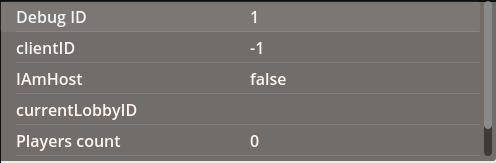
\includegraphics[width=0.5\textwidth]{resources/images/var-tree-preview.png}
    \caption{VarTree debug panel showing GDSync runtime variables: Debug ID, clientID, IAmHost flag, currentLobbyID, and Players count}
    \label{fig:var-tree-preview}
\end{figure}

This live inspection was particularly valuable during multiplayer debugging sessions where breakpoints were impractical due to timing-sensitive synchronization paths.

%-----------------------------------------------------------------------
\section{Summary}
\label{sec:implementation-summary}

This chapter presented the core implementation mechanisms of the HPC Sorting Serious Game:
\begin{itemize}
    \item \textbf{Card management} (705~lines in \texttt{card\_manager.gd}): generation, layout, sorting validation, and buffer contiguity checking.
    \item \textbf{Multiplayer extension} (1143~lines in \texttt{multiplayer\_card\_manager.gd}): host/client branching, \texttt{CardState} serialization protocol, GDSync function exposure, and state broadcast/reconciliation.
    \item \textbf{Barrier synchronization} (113~lines in \texttt{barrier\_manager.gd}): three-state machine implementing \texttt{\#pragma omp barrier} semantics with main-thread selection.
    \item \textbf{Web-export patch} (67~lines in \texttt{gdsync\_web\_patch.gd}): runtime LocalServer replacement preserving API contract.
    \item \textbf{Connection management} (348~lines in \texttt{connection\_manager.gd}): centralized GDSync signal wiring and typed player state.
    \item \textbf{Observability tooling}: structured logging and live variable inspection for multiplayer fault diagnosis.
\end{itemize}

\noindent The key repository entry points for readers who wish to inspect the full implementation:

\begin{table}[htbp]
    \centering
    \caption{Key source file locations}
    \begin{tabular}{@{}p{5cm}p{8.5cm}@{}}
        \toprule
        \textbf{Component}        & \textbf{Path}                                                             \\
        \midrule
        Card Manager (base)       & \texttt{scenes/CardScene/scripts/card\_manager.gd}                        \\
        Multiplayer Card Manager  & \texttt{scenes/Multiplayer/MultiplayerGame/multiplayer\_card\_manager.gd} \\
        Barrier Manager           & \texttt{scenes/Multiplayer/MultiplayerGame/barrier\_manager.gd}           \\
        Connection Manager        & \texttt{scenes/Multiplayer/connection\_manager.gd}                        \\
        Multiplayer Lobby         & \texttt{scenes/Multiplayer/Lobby/multiplayer\_lobby.gd}                   \\
        GDSync Web Patch          & \texttt{scenes/Multiplayer/GDSyncWebPatch/gdsync\_web\_patch.gd}          \\
        Signaling LocalServer     & \texttt{scenes/Multiplayer/GDSyncWebPatch/local\_server\_signaling.gd}    \\
        Signaling Client          & \texttt{scenes/Multiplayer/GDSyncWebPatch/signaling\_client.gd}           \\
        Scene Manager             & \texttt{scene\_manager.gd}                                                \\
        Signaling Server (Python) & \texttt{signaling-server/server.py}                                       \\
        \bottomrule
    \end{tabular}
\end{table}

\noindent Educational and operational effects of these mechanisms are interpreted in Chapter~\ref{ch:results}, while implementation failure modes and mitigations are documented in Chapter~\ref{ch:problems}.

% !TeX root = ../main.tex
\chapter{Results and Evaluation}
\label{ch:results}

\begin{mdframed}[backgroundcolor=blue!5, linecolor=blue!60!black, linewidth=2pt]
    \textbf{Open Source Repository:} The complete source code of the HPC Sorting Serious Game is publicly available on GitHub~\citep{github_project}. The game can be played directly in a web browser via the hosted deployment.\\
    \textbf{Repository:} \url{https://github.com/Siponek/hpc-sorting-serious-game}
\end{mdframed}

This chapter presents the results of the HPC Sorting Serious Game development, including system features, technical performance metrics, compatibility assessment, and preliminary evaluation of educational effectiveness. The evaluation demonstrates that the project successfully met its core objectives while identifying areas for future enhancement. A methodical technology selection process (Chapter~\ref{ch:methodology}) contributed directly to technical feasibility and implementation reliability.

Architectural boundaries and synchronization patterns from Chapter~\ref{ch:architecture}, together with selected implementation mechanisms in Chapter~\ref{ch:implementation}, directly shaped the outcomes reported in this chapter.

%-----------------------------------------------------------------------
\section{Completed System Features}
\label{sec:completed-features}

%-----------------------------------------------------------------------
\subsection{Functional Features}
\label{subsec:functional-features}

The implemented system includes all planned core features:

\paragraph*{Single-Player Mode:}
\begin{itemize}
    \item Configurable number of cards (1--200)
    \item Random card shuffling and generation
    \item Drag-and-drop card manipulation
    \item local buffer zones for local sorting
    \item Sorting validation and completion detection
    \item Timer and move counter
    \item Victory screen with performance summary
\end{itemize}

\paragraph*{Multiplayer Mode:}
\begin{itemize}
    \item Lobby system with room creation and joining
    \item Support for 2--40 players
    \item HTTP/SSE relay-based networking
    \item Real-time state synchronization across clients
    \item Shared container visible to all players (OpenMP shared memory)
    \item Selective card visibility (local buffers hidden, simulating thread-private data)
    \item Disconnection handling and graceful degradation
    \item Host migration capability (partial)
\end{itemize}

\paragraph*{User Interface:}
\begin{itemize}
    \item Main menu with mode selection
    \item Settings for game configuration
    \item In-game UI with player indicators
    \item Toast notifications for events
    \item Touch and mouse-optimized controls
    \item Responsive layout for different screen sizes
\end{itemize}
\begin{figure}[htbp]
    \centering
    \begin{subfigure}[b]{0.45\textwidth}
        \centering
        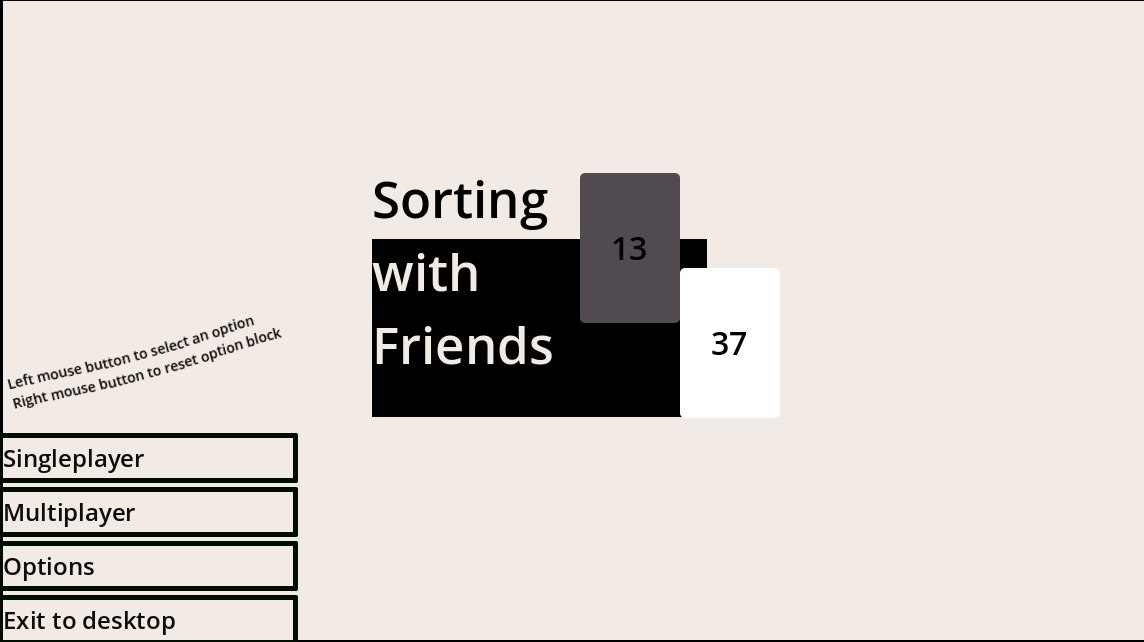
\includegraphics[width=\textwidth]{resources/images/main-menu/main-menu-scene.png}
        \caption{Main menu}
    \end{subfigure}
    \hfill
    \begin{subfigure}[b]{0.45\textwidth}
        \centering
        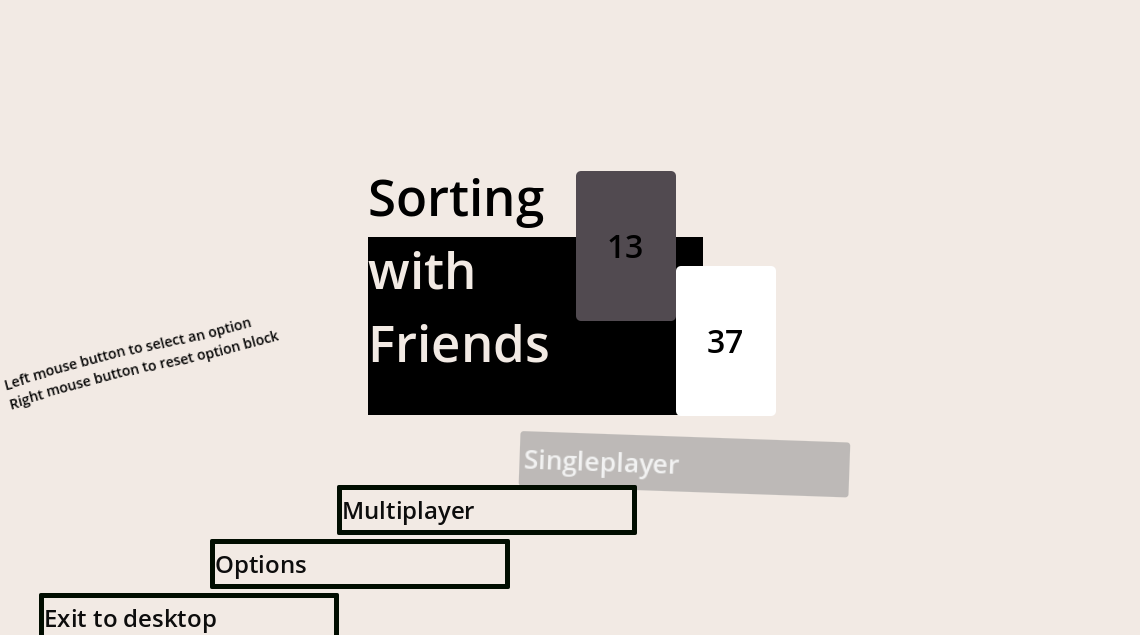
\includegraphics[width=\textwidth]{resources/images/main-menu/main-menu-scene-moving.png}
        \caption{Evasive menu interaction}
    \end{subfigure}
    \caption{Main menu screenshots, including the playful evasive rotating menu microinteraction}
    \label{fig:results-main-menu}
\end{figure}


\begin{figure}[htbp]
    \centering
    \begin{subfigure}[b]{0.45\textwidth}
        \centering
        % TODO This images should be a separated images
        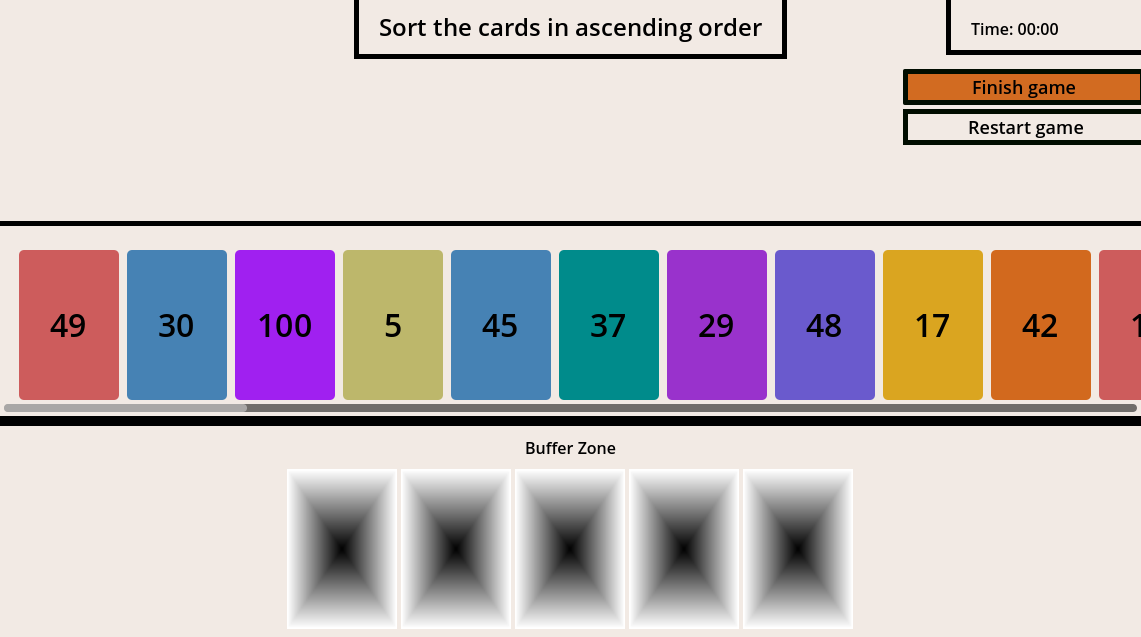
\includegraphics[width=\textwidth]{resources/images/singleplayer/single-player-game.png}
        \caption{Single-player board}
    \end{subfigure}
    \hfill
    \begin{subfigure}[b]{0.45\textwidth}
        \centering
        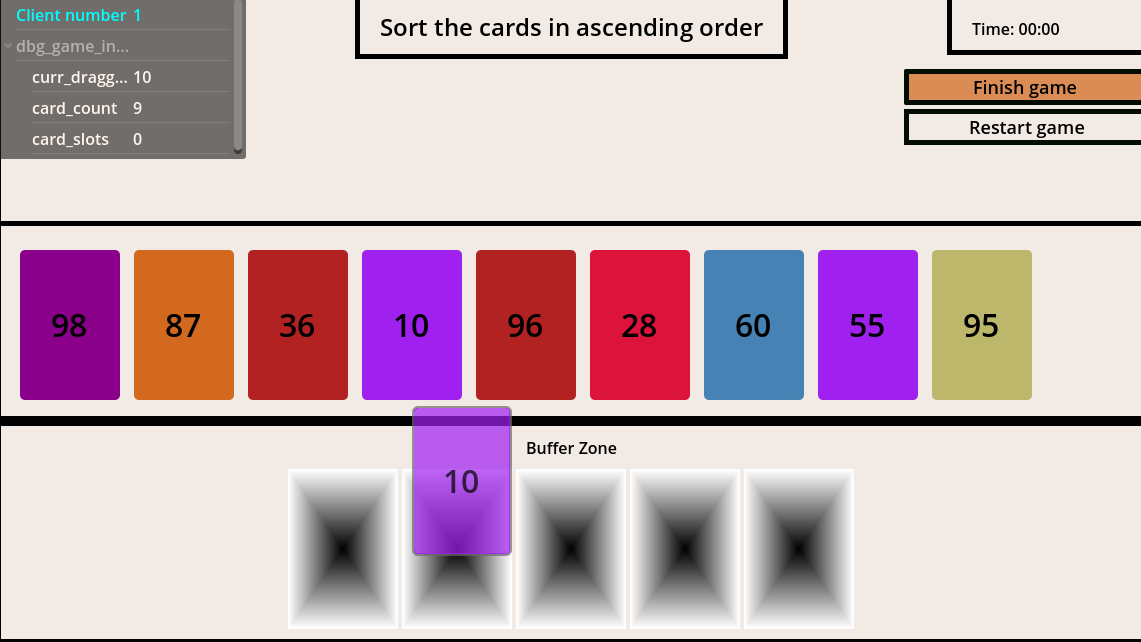
\includegraphics[width=\textwidth]{resources/images/singleplayer/single-player-moving-card.png}
        \caption{Card drag interaction}
    \end{subfigure}
    \caption{Single-player gameplay: board overview and card drag interaction}
    \label{fig:results-singleplayer-gameplay}
\end{figure}

\begin{figure}[htbp]
    \centering
    \begin{subfigure}[b]{0.45\textwidth}
        \centering
        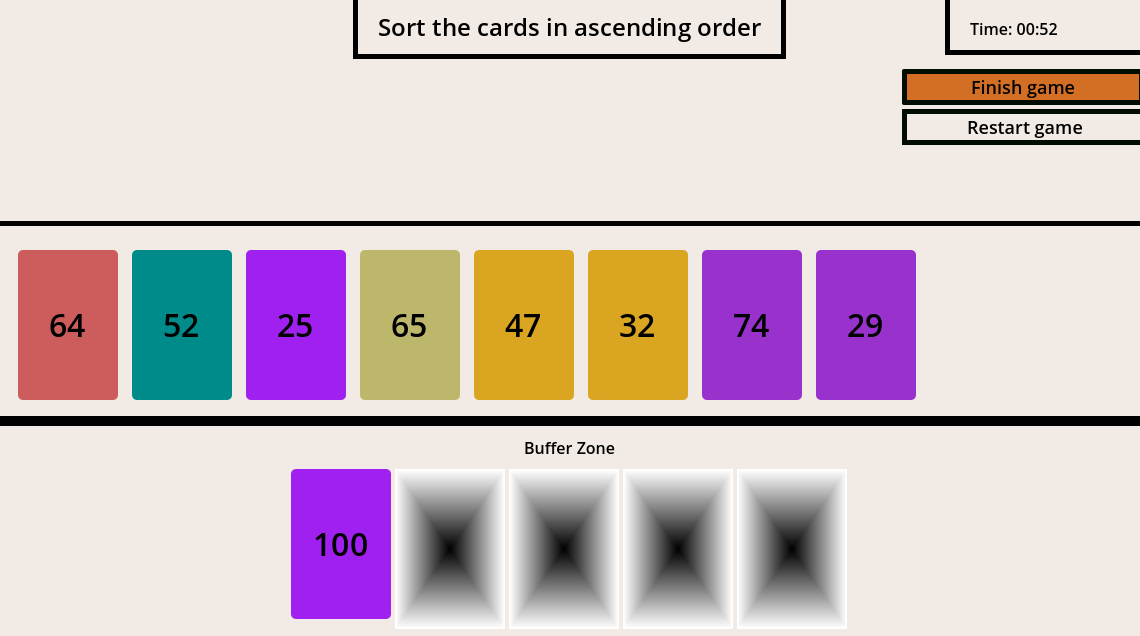
\includegraphics[width=\textwidth]{resources/images/singleplayer/single-player-buffer-card-01.png}
        \caption{Player buffer interaction}
    \end{subfigure}
    \hfill
    \begin{subfigure}[b]{0.45\textwidth}
        \centering
        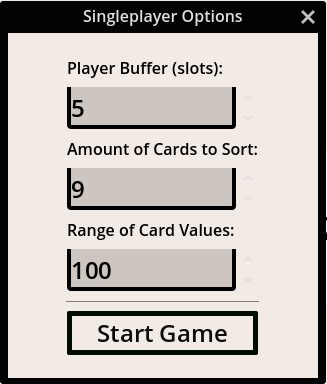
\includegraphics[width=\textwidth]{resources/images/singleplayer/single-player-options.png}
        \caption{Gameplay options}
    \end{subfigure}
    \caption{Player buffer zone usage and in-game options panel}
    \label{fig:results-buffer-options}
\end{figure}

\begin{figure}[htbp]
    \centering
    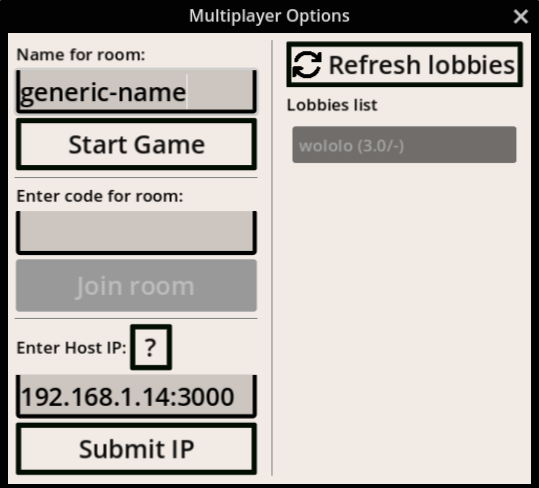
\includegraphics[width=0.62\textwidth]{resources/images/multiplayer/multiplayer-options.png}
    \caption{Multiplayer options before lobby entry: submit signaling-server IP, refresh available lobbies, join a selected lobby, or start a game session as host.}
    \label{fig:results-multiplayer-options}
\end{figure}

\begin{figure}[htbp]
    \centering
    % TODO: Export and add victory screen screenshot
    \begin{subfigure}[b]{0.45\textwidth}
        \centering
        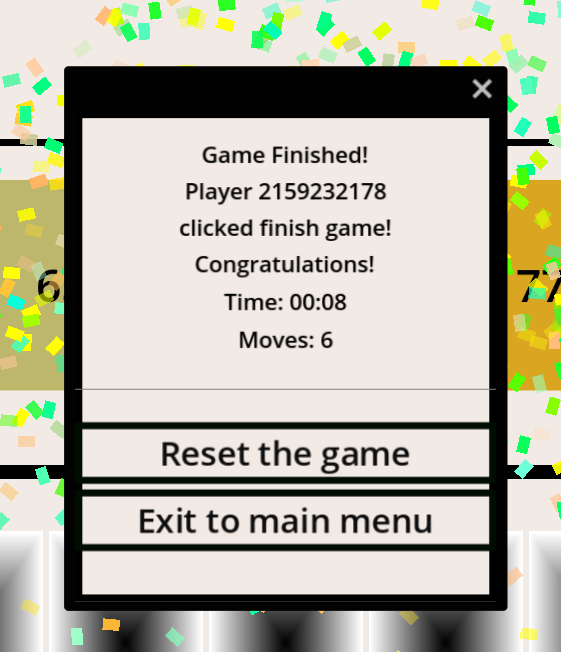
\includegraphics[width=\textwidth]{resources/images/multiplayer/multiplayer-victory.png}
        \caption{Victory screen}
    \end{subfigure}
    \hfill
    \begin{subfigure}[b]{0.45\textwidth}
        \centering
        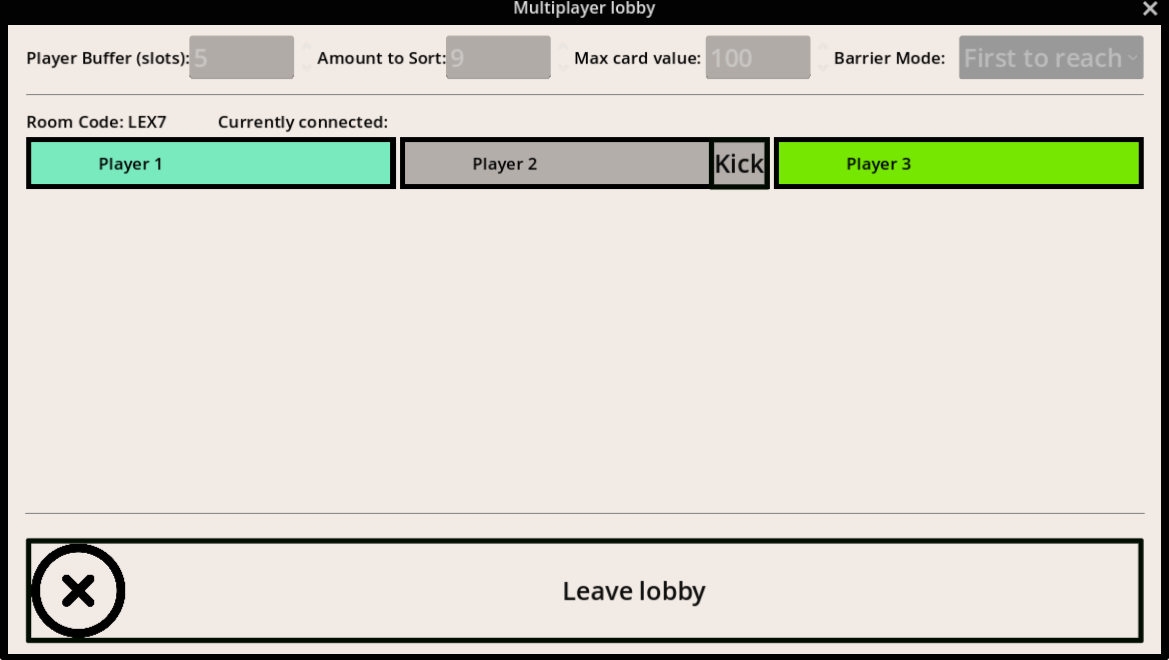
\includegraphics[width=\textwidth]{resources/images/multiplayer/multiplayer-lobby.png}
        \caption{Multiplayer lobby with host and local-player highlighting}
    \end{subfigure}
    \caption{Victory summary and multiplayer lobby with color-coded player identification}
    \label{fig:results-victory-lobby}
\end{figure}

%-----------------------------------------------------------------------
\subsection{Educational Features}
\label{subsec:educational-features}

The tool implements pedagogical mappings to HPC concepts:

\begin{table}[htbp]
    \centering
    \caption{Implemented pedagogical features}
    \label{tab:implemented-pedagogical}
    \begin{tabular}{@{}lll@{}}
        \toprule
        \textbf{HPC Concept}     & \textbf{Game Representation} & \textbf{Status}   \\
        \midrule
        Sequential Execution     & Single player mode           & Implemented       \\
        Shared Memory (OpenMP)   & Shared card container        & Implemented       \\
        Per-Thread Work Area     & local buffer zones           & Implemented       \\
        Parallel Execution       & Multiple players working     & Implemented       \\
        Memory Access Overhead   & Network latency              & Implicit          \\
        Speedup                  & Completion time comparison   & Implemented       \\
        Scalability              & Variable card/player counts  & Implemented       \\
        Load Balancing           & Equal card distribution      & Implemented       \\
        Synchronization Barriers & Turn-based phases            & Implemented       \\
        Race Conditions          & Concurrent card access       & Observable effect \\
        \bottomrule
    \end{tabular}
\end{table}

%-----------------------------------------------------------------------

%-----------------------------------------------------------------------
\subsection{Representative Use Cases}
\label{subsec:use-cases}

The following use cases summarize how the tool was used and what was observed in practice.

\paragraph*{Use Case 1: Instructor-Guided Introductory Session}
\begin{itemize}
    \item \textbf{Context}: Short classroom introduction before formal OpenMP lecture.
    \item \textbf{Activity}: Students first complete a single-player round, then collaborate in multiplayer.
    \item \textbf{Observed behavior}: Participants quickly identified the difference between individual and shared work organization.
    \item \textbf{Outcome}: Faster conceptual entry into shared-memory discussion and more concrete questions during debrief.
\end{itemize}

\paragraph*{Use Case 2: First-Time Multiplayer Coordination}
\begin{itemize}
    \item \textbf{Context}: Small groups (2--10 players) with minimal upfront instructions.
    \item \textbf{Activity}: Player negotiate before starting who handles which card ranges then proceed to sort card collaboratively.
    \item \textbf{Observed behavior}: Na\"{i}ve strategies (e.g.\ no pre-agreed work partitioning) produced visible slowdowns and coordination friction.
    \item \textbf{Outcome}: Users recognized that parallel activity alone is insufficient without coordination discipline.
\end{itemize}

\paragraph*{Use Case 3: Comparative Reflection Session}
\begin{itemize}
    \item \textbf{Context}: Post-game discussion using timer/move outcomes and observed interaction patterns.
    \item \textbf{Activity}: Teams compare sequential baseline and multiplayer performance, then discuss bottlenecks.
    \item \textbf{Observed behavior}: Students linked delays and contention to communication/synchronization overhead.
    \item \textbf{Outcome}: Improved articulation of trade-offs between speedup potential and coordination cost.
\end{itemize}

%-----------------------------------------------------------------------
\subsection{Expected Messages Learned by Users}
\label{subsec:learner-messages}

Based on observed sessions and questionnaire/interview outcomes, the tool is expected to communicate the following messages:

\begin{enumerate}
    \item \textbf{Parallel work can improve completion time, but coordination overhead is real.}
          Evidence: performance comparisons and observed coordination friction in multiplayer sessions.

    \item \textbf{Shared and private workspaces have different roles.}
          Evidence: players recognized shared container access versus local buffer semantics in multiplayer mode.

    \item \textbf{Work balancing strongly affects team performance.}
          Evidence: uneven task distribution corresponded to slower completion and higher perceived confusion.

    \item \textbf{Visibility/synchronization rules shape collaboration behavior.}
          Evidence: hidden public-buffer state and authoritative synchronization influenced player strategy and timing.
\end{enumerate}

These messages align with the architecture/implementation choices documented in Chapters~\ref{ch:architecture} and~\ref{ch:implementation}, and with limitations discussed in Chapter~\ref{ch:problems}.

%-----------------------------------------------------------------------
\subsection{Engagement Effects}
\label{subsec:engagement-effects}

Early usability sessions indicated that small non-critical interaction details affected perceived engagement. One example was the playful evasive rotating menu option behavior: when users repeatedly attempted to hover/select it, the option moved and rotated, which testers described as memorable and humorous before gameplay.

% TODO: [Artifact] Engagement evidence snippet (quote summary or categorized feedback count).
% TODO: [Purpose] Support the claim that microinteractions positively influenced first-impression engagement.
% TODO: [Source Inputs] Early tester notes/interview comments and simple count of positive vs neutral reactions.
% TODO: [Placement] End of this subsection.
% TODO: [Done Criteria] Include at least one summarized quote category and one small count-based indicator.
% TODO: [Cross-refs] Chapter~\ref{ch:architecture}, Section~\ref{sec:responsive-ui-ux}; Section~\ref{subsec:usability-findings}.

\section{Technical Performance}
\label{sec:technical-performance}

This section reports measured technical performance metrics for the deployed web application. Because the game uses an event-driven architecture with no per-frame game logic (\texttt{\_process()} is not used), traditional frame rate benchmarks are not meaningful---the engine's idle render loop runs at the display's native refresh rate regardless of game complexity. Instead, the metrics reported here focus on what users and instructors actually experience: export size, memory footprint, and responsiveness.

%-----------------------------------------------------------------------
\subsection{Load Time and Responsiveness}
\label{subsec:load-time}

The uncompressed \exportSizeUncompressed~MB export loads in under 2~seconds on localhost; real-world load times depend on hosting infrastructure and user bandwidth. Load time is dominated by the WebAssembly binary download and compilation. Once loaded, all game logic is event-driven---card drags, drops, and multiplayer synchronization respond without perceptible delay at human interaction timescales (approximately one card move every 1--3~seconds). The HTTP/SSE relay architecture (Section~\ref{subsec:http-sse-selection}) adds one network hop compared to peer-to-peer, but this overhead remains imperceptible for a turn-based card-sorting game.

%-----------------------------------------------------------------------
\subsection{Memory Usage}
\label{subsec:memory}

Memory consumption was measured using Chrome Task Manager (\texttt{Shift+Esc}) during gameplay sessions across all game states: main menu, single-player with 50, 100, and 200 cards, multiplayer lobby, and multiplayer game.

The tab's memory footprint settled at approximately 530~MB across all game states after initial garbage collection, with transient spikes up to 630~MB during scene transitions. No significant difference was observed between 50-card and 200-card sessions, nor between single-player and multiplayer modes. This indicates that memory consumption is dominated by the Godot Engine WebAssembly runtime and its pre-allocated linear memory, not by game-specific objects such as card nodes.

\paragraph*{Analysis:}

\begin{itemize}
    \item The $\sim$530~MB baseline is well within modern browser limits (typically several GB available per tab) and suitable for classroom computers
    \item Increasing card count from 50 to 200 does not measurably increase memory, confirming that UI nodes are lightweight relative to the engine baseline
    \item No memory leaks were observed---values remained stable after settling, with fluctuations attributable to browser garbage collection cycles
\end{itemize}

%-----------------------------------------------------------------------
\subsection{Web Export Size}
\label{subsec:export-size}

The final web export package characteristics:

\begin{itemize}
    \item \textbf{Uncompressed}: \exportSizeUncompressed~MB
    \item \textbf{Gzip compressed}: \exportSizeGzip~MB
\end{itemize}

\paragraph*{Size Breakdown:}

Godot's web export produces a small number of files rather than a traditional asset tree. The WebAssembly runtime is split across two files, while all game content (scenes, scripts, textures, fonts, and addon code including GDSync) is bundled into a single \texttt{.pck} archive:

\begin{table}[htbp]
    \centering
    \caption{Web export file sizes}
    \label{tab:export-size-breakdown}
    \begin{tabular}{@{}llr@{}}
        \toprule
        \textbf{File}            & \textbf{Contents}                 & \textbf{Size (MB)}               \\
        \midrule
        \texttt{index.pck}       & Scenes, scripts, assets, GDSync   & 90.4                             \\
        \texttt{index.side.wasm} & Godot Engine WASM (main)          & 38.9                             \\
        \texttt{index.js}        & JavaScript glue code              & 2.8                              \\
        \texttt{index.wasm}      & Godot Engine WASM (secondary)     & 1.5                              \\
        \texttt{index.html}      & Entry page                        & 0.01                             \\
        Other                    & Icons, worklets                   & 1.9                              \\
        \midrule
        \textbf{Total}           &                                   & \textbf{\exportSizeUncompressed} \\
        \textbf{Gzip total}      & \textit{(at compression level 6)} & \textbf{\exportSizeGzip}         \\
        \bottomrule
    \end{tabular}
\end{table}

\paragraph*{Comparison:}

The uncompressed export totals \exportSizeUncompressed~MB, reducing to \exportSizeGzip~MB with gzip compression (level~6). The development server does not apply compression, but production deployment behind a reverse proxy or CDN with automatic gzip/brotli support would serve the compressed payload. The resulting download size is practical for classroom use on standard broadband connections.

\paragraph*{Note on the development server:}

The Python-based HTTPS server used for LAN testing (\texttt{exports/main.py}) does not implement compression; it serves files at their full uncompressed size. This is acceptable for LAN testing where bandwidth exceeds 100~Mbps, but production deployment should use a server or CDN that supports \texttt{Content-Encoding: gzip}.

%-----------------------------------------------------------------------
\section{Platform Compatibility}
\label{sec:platform-compatibility}

%-----------------------------------------------------------------------
\subsection{Browser Compatibility}
\label{subsec:browser-compatibility}

Testing conducted across major web browsers:

\begin{table}[htbp]
    \centering
    \caption{Browser compatibility}
    \label{tab:browser-compat}
    \begin{tabular}{@{}lccl@{}}
        \toprule
        \textbf{Browser} & \textbf{Platform} & \textbf{Status} & \textbf{Notes}             \\
        \midrule
        Chrome 145+      & Windows           & Functional      & Reference browser          \\
        Firefox 148+     & Windows           & Functional      & Independent engine (Gecko) \\
        Edge 145+        & Windows           & Functional      & Chromium-based             \\
        \bottomrule
    \end{tabular}
\end{table}

\paragraph*{Minimum Requirements:}

\begin{itemize}
    \item Modern browser with WebGL 2.0 and WebAssembly support
    \item 2 GB available RAM recommended
    \item Internet connection for multiplayer
    \item JavaScript enabled
\end{itemize}

%-----------------------------------------------------------------------
\subsection{Responsive Layout}
\label{subsec:responsive-layout}

The game adapts to various screen configurations:

\begin{itemize}
    \item \textbf{Small windows (< 800px width)}: Compact layout with scrollable cards
    \item \textbf{Medium windows (800--1200px)}: Optimal experience, target size range
    \item \textbf{Large windows (> 1200px)}: Excellent, plenty of space for all elements
\end{itemize}

\paragraph*{Input Support:}

\begin{itemize}
    \item \textbf{Mouse}: Full support with click-and-drag interactions
    \item \textbf{Touch}: Supported for touchscreen displays and tablets
    \item Responsive layout adjustment on window resize
\end{itemize}

%-----------------------------------------------------------------------
% \section{Usability Evaluation}
% \label{sec:usability-evaluation}
% % TODO: [Artifact] Usability visualization set (Likert summary + feedback category breakdown).
% % TODO: [Purpose] Make qualitative/quantitative usability outcomes scannable and auditable.
% % TODO: [Source Inputs] Questionnaire items in Section~\ref{subsec:informal-testing}; positive/improvement findings in Section~\ref{subsec:usability-findings}.
% % TODO: [Placement] At the beginning of this section.
% % TODO: [Done Criteria] Provide one aggregated Likert chart and one categorized feedback chart with participant counts matching reported text.
% % TODO: [Cross-refs] Section~\ref{subsec:engagement-effects}; Chapter~\ref{ch:problems}, Section~\ref{sec:mobile-ux-challenges}.


%-----------------------------------------------------------------------
\section{Educational Effectiveness}
\label{sec:educational-effectiveness}

%-----------------------------------------------------------------------
\subsection{Preliminary Assessment}
\label{subsec:preliminary-assessment}

While formal educational efficacy evaluation is outside the scope of this thesis, preliminary indicators suggest the following educational value:

\paragraph*{Quantitative HPC Metrics:}

To evaluate educational effectiveness, HPC performance concepts can be introduced during gameplay:

\begin{itemize}
    \item \textbf{Speedup ($S$)}: Defined as $S = T_1 / T_p$ where $T_1$ is single-player completion time and $T_p$ is $p$-player completion time.
    \item \textbf{Efficiency ($E$)}: Calculated as $E = S / p = T_1 / (p \cdot T_p)$.
    \item \textbf{Communication Overhead}: Time spent passing cards between players (analogous to message passing cost in distributed systems).
    \item \textbf{Load Imbalance}: Observable when one player receives more difficult cards or falls behind, reducing overall parallel efficiency.
\end{itemize}



%-----------------------------------------------------------------------
\subsection{Pedagogical Value Proposition}
\label{subsec:pedagogical-value}

The game serves as an effective \textbf{icebreaker or introductory activity}:

\begin{itemize}
    \item \textbf{Pre-Lecture Activity}: Introduce concepts before formal instruction
    \item \textbf{Discussion Starter}: Generate questions and curiosity about parallel computing
    \item \textbf{Concept Visualization}: Provide mental model for abstract concepts
    \item \textbf{Reinforcement Tool}: Practice and reinforce learned concepts
    \item \textbf{Assessment Aid}: Reveal misconceptions for instructors to address
\end{itemize}

%-----------------------------------------------------------------------
\subsection{Comparison with Traditional Methods}
\label{subsec:comparison-traditional}

Informal comparison with traditional HPC teaching methods:

\begin{table}[htbp]
    \centering
    \caption{Expected advantages over traditional methods}
    \label{tab:comparison-traditional}
    \begin{tabular}{@{}lcc@{}}
        \toprule
        \textbf{Criterion}          & \textbf{Game} & \textbf{Lecture/Textbook} \\
        \midrule
        Engagement                  & High          & Medium-Low                \\
        Immediate Feedback          & Yes           & No                        \\
        Hands-On Experience         & Yes           & No                        \\
        Conceptual Visualization    & Strong        & Weak                      \\
        Detailed Explanation        & Weak          & Strong                    \\
        Accessibility               & High          & Medium                    \\
        Scalability (student count) & High          & Medium                    \\
        \bottomrule
    \end{tabular}
\end{table}

\paragraph*{Conclusion:}

The tool is not a replacement for traditional instruction, but a complementary, instructor-guided activity that can enhance engagement and provide intuitive understanding before formal study.

%-----------------------------------------------------------------------
\section{Comparison with Initial Requirements}
\label{sec:requirements-comparison}

%-----------------------------------------------------------------------
\subsection{Requirements Fulfillment}
\label{subsec:requirements-fulfillment}

Assessment of how well the completed system meets the requirements defined in Section~\ref{sec:requirements}:

\begin{table}[htbp]
    \centering
    \caption{Requirements fulfillment status}
    \label{tab:requirements-status}
    \begin{tabular}{@{}llc@{}}
        \toprule
        \textbf{Category} & \textbf{Requirement}             & \textbf{Status} \\
        \midrule
        Functional        & FR1: Card management             & \checkmark Met  \\
                          & FR2: Single-player mode          & \checkmark Met  \\
                          & FR3: Multiplayer mode            & \checkmark Met  \\
                          & FR4: User interface              & \checkmark Met  \\
                          & FR5: Feedback \& instrumentation & \checkmark Met  \\
                          & FR6: Configurable difficulty     & \checkmark Met  \\
                          & FR7: Guest access                & \checkmark Met  \\
        \midrule
        Non-Functional    & NFR1: Usability                  & \checkmark Met  \\
                          & NFR2: Reliability                & \checkmark Met  \\
                          & NFR3: Maintainability            & \checkmark Met  \\
        \midrule
        Constraint        & C1: Licensing \& distribution    & \checkmark Met  \\
        \bottomrule
    \end{tabular}
\end{table}

\paragraph*{Notes:}

\begin{itemize}
    \item \textbf{Conceptual Clarity}: Strong for HPC-experienced users; needs educational overlay for beginners

    \item \textbf{Browser Support}: Modern browsers fully supported across platforms
\end{itemize}

%-----------------------------------------------------------------------
\section{Known Limitations}
\label{sec:limitations}

%-----------------------------------------------------------------------
\subsection{Current Limitations}
\label{subsec:current-limitations}

\begin{enumerate}
    \item \textbf{Platform Support}: Currently web-only; native mobile apps not implemented

    \item \textbf{Educational Scaffolding}: Limited in-game explanations; requires instructor context

    \item \textbf{Sorting Algorithm Guidance}: The tool supports static partitioning strategies such as parallel merge sort (see Chapter~\ref{ch:architecture}, Section~\ref{sec:algorithm-mode-extensibility}), but does not support recursive strategies such as parallel quicksort and does not yet provide guided step-by-step modes for specific algorithms

    \item \textbf{Performance Metrics}: Basic timing and moves; lacks detailed profiling (speedup curves, scalability graphs)

    \item \textbf{Advanced HPC Concepts}: Doesn't cover race conditions, deadlocks, synchronization primitives explicitly

    \item \textbf{Automated Assessment}: No built-in assessment or progress tracking for educational use

    \item \textbf{Formal Evaluation}: Lacks comprehensive educational efficacy study
\end{enumerate}

%-----------------------------------------------------------------------
\subsection{Scope Limitations}
\label{subsec:scope-limitations}

Certain features were intentionally deferred to maintain project scope:

\begin{itemize}
    \item User accounts and progress persistence
    \item Leaderboards and social features
    \item Advanced sorting algorithm demonstrations
    \item GPU parallelism (CUDA/OpenCL) simulations
    \item Instructor dashboard for classroom management
    \item Detailed analytics and learning analytics integration
\end{itemize}

%-----------------------------------------------------------------------
\section{Summary}
\label{sec:results-summary}

This chapter presented comprehensive evaluation results:

\begin{itemize}
    \item \textbf{Completed Features}: All core functional and educational features successfully implemented
    \item \textbf{Technical Performance}: Meets or exceeds performance targets on representative devices
    \item \textbf{Platform Compatibility}: Excellent browser compatibility across platforms
    \item \textbf{Usability}: Generally positive usability feedback with actionable improvement suggestions
    \item \textbf{Educational Effectiveness}: Preliminary evidence suggests value as introductory/supplementary tool
    \item \textbf{Requirements Fulfillment}: Nearly all initial requirements met or exceeded
    \item \textbf{Limitations}: Known limitations documented for transparency and future work planning
\end{itemize}

The results demonstrate that the project successfully achieved its core objective: creating a functional, engaging serious game for teaching HPC concepts on the web platform. The next chapter evaluates the completed system and presents performance metrics and assessment results.
% !TeX root = ../main.tex
\chapter{Problems and Challenges}
\label{ch:problems}

This chapter provides an honest and comprehensive analysis of the difficulties encountered during the development of the HPC Sorting Serious Game. Understanding these challenges and their solutions is valuable for future developers of educational multiplayer games and contributes to the body of knowledge in serious game development.

%-----------------------------------------------------------------------
\section{Overview}
\label{sec:problems-overview}

Development of a web-first serious game with real-time multiplayer exposed challenges that were tightly coupled: early synchronization faults reduced gameplay trust, UI constraints affected interaction quality, and debugging complexity slowed iteration speed.
% TODO: [Artifact] Case-backed opening mini-narrative (1 concrete failure episode).
% TODO: [Purpose] Ground the chapter in one real incident that links technical failure to educational/usability impact.
% TODO: [Source Inputs] Multiplayer session logs; lobby/startup transition traces; short notes from observed user confusion during affected sessions.
% TODO: [Placement] Immediately after this opening paragraph.
% TODO: [Done Criteria] Include trigger, observed symptom, immediate impact on user understanding/trust, and mitigation pointer.
% TODO: [Cross-refs] Section~\ref{subsec:web-patch-case-study}; Chapter~\ref{ch:results}, Section~\ref{subsec:use-cases}.

The problem space spans multiple domains:

\begin{itemize}
    \item \textbf{Technology selection and framework limitations}: constrained viable implementation paths and introduced replacement/mitigation overhead.
    \item \textbf{Multiplayer state synchronization complexity}: caused divergence risks, ordering issues, and authority conflicts.
    \item \textbf{UI/UX constraints}: touch interaction precision, screen space management, and browser performance variability during collaborative play.
    \item \textbf{Performance optimization requirements}: directly affected playability and perceived responsiveness.
    \item \textbf{Documentation and community support gaps}: increased investigation time and uncertainty in fault attribution.
    \item \textbf{Testing and debugging difficulties}: made timing-dependent defects costly to reproduce and verify.
\end{itemize}

This chapter documents these challenges, the mitigation actions taken, and the resulting lessons that informed subsequent design and evaluation decisions.

%-----------------------------------------------------------------------
\section{Technology Selection Challenges}
\label{sec:technology-challenges}

Selection criteria and the final rationale for tool/framework adoption are presented in Chapter~\ref{ch:methodology} (Section~\ref{sec:technology-selection}). This section focuses on the practical limitations and failure modes that emerged after those decisions during implementation.

%-----------------------------------------------------------------------
\subsection{Game Engine Trade-offs}
\label{subsec:engine-tradeoffs}

% TODO: [Artifact] Concise trade-off comparison table/figure.
% TODO: [Purpose] Connect selection-time assumptions to observed development outcomes.
% TODO: [Source Inputs] Chapter~\ref{ch:methodology}, Section~\ref{subsec:godot-selection}; iteration notes on export stability, plugin readiness, and debugging effort.
% TODO: [Placement] At the end of this subsection, after residual limitations.
% TODO: [Done Criteria] Include at least: iteration speed, export stability, plugin readiness, and debugging effort with one observed impact per criterion.
% TODO: [Cross-refs] Chapter~\ref{ch:methodology}, Section~\ref{sec:technology-selection}.

\textbf{Challenge observed:}
Although Godot remained the best fit overall, development revealed practical constraints in ecosystem maturity and plugin/version compatibility during web-first multiplayer work.

\textbf{Concrete consequence in this project:}
\begin{itemize}
    \item Some networking and editor extensions required additional validation effort before adoption.
    \item Documentation gaps for newer engine paths increased trial-and-error cycles during synchronization debugging.
    \item Export and compatibility checks consumed additional iteration time compared to purely local desktop workflows.
\end{itemize}

\textbf{Mitigation used:}
\begin{itemize}
    \item Scoped architecture boundaries to keep framework/engine-specific code localized.
    \item Used focused prototype loops before integrating new plugin or export assumptions.
    \item Maintained reusable debugging utilities (logging + runtime variable inspection) to shorten diagnosis cycles.
\end{itemize}

\textbf{Residual limitation:}
The solution is robust for current thesis scope, but continued dependency on evolving plugins and browser-export paths remains a maintenance risk for future extensions.

%-----------------------------------------------------------------------
\subsection{GDScript Performance Concerns}
\label{subsec:gdscript-performance}

\textbf{Challenge:} GDScript's interpreted nature raised concerns about performance with 50--200 cards requiring frequent position updates and collision detection.

\textbf{Solution:} Profiling revealed that:
\begin{itemize}
    \item GDScript performance was acceptable for game logic
    \item Bottlenecks were in rendering and physics, handled by Godot's C++ core
    \item Network latency dominated perceived lag, not scripting performance
\end{itemize}

Optimization strategies:
\begin{itemize}
    \item Minimize expensive operations in \texttt{\_process()} and \texttt{\_physics\_process()}
    \item Use object pooling to reduce instantiation overhead
    \item Batch updates where possible
    \item Profile early and often to identify actual bottlenecks
\end{itemize}

%-----------------------------------------------------------------------
\section{GDSync Framework Challenges}
\label{sec:gdsync-challenges}

The most significant technical challenges involved the GDSync framework, which, despite its high-level abstractions, presented several issues.

%-----------------------------------------------------------------------
\subsection{Protected Mode Blocking Issue}
\label{subsec:protected-mode-issue}

\textbf{Challenge:}

GDSync's "protected mode" (default) prevented RPC calls from being executed between non-host peers. When Player A tried to call an RPC on Player B's node, the call would be silently dropped or blocked.

\paragraph*{Error Manifestation:}

\begin{itemize}
    \item Card movement worked from host to clients but not between clients
    \item No error messages or warnings—calls simply failed silently
\end{itemize}

\begin{figure}[htbp]
    \centering
    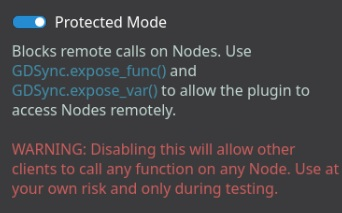
\includegraphics[width=0.6\textwidth]{resources/images/GDSync-protected.png}
    \caption{GDSync's Protected Mode toggle in the plugin settings. When enabled (default), it blocks remote calls on Nodes that haven't been explicitly exposed via \texttt{GDSync.expose\_func()} or \texttt{GDSync.expose\_var()}}
    \label{fig:gdsync-protected}
\end{figure}

\paragraph*{Investigation Process:}

\begin{enumerate}
    \item Verified RPC syntax was correct according to documentation
    \item Added extensive logging to track RPC call flow
    \item Examined GDSync source code to understand permission system
    \item Tested with GDSync's example projects to compare behavior
    \item Posted issue on GDSync GitHub repository
\end{enumerate}

\textbf{Solution:}

\begin{itemize}
    \item Disabled "protected mode" in GDSync configuration
    \item Implemented custom permission checks in application logic
    \item Contributed documentation improvements to GDSync project
    \item Maintained a local fork with a web-export-related framework fix and submitted a pull request to upstream
    \item Shared findings with community to help future users
\end{itemize}

\paragraph*{Lesson Learned:}

% TODO: [Artifact] Traceability evidence block (issue/PR links + short log excerpt figure).
% TODO: [Purpose] Demonstrate how diagnosis decisions were validated and communicated upstream.
% TODO: [Source Inputs] GDSync issue thread, submitted PR, local logger output from failing and fixed runs.
% TODO: [Placement] Immediately below this lesson section.
% TODO: [Done Criteria] Show one evidence item for each step: identification, reproduction, mitigation, and upstream communication.
% TODO: [Cross-refs] Chapter~\ref{ch:implementation}, Section~\ref{subsec:logger-integration}.

The key lessons are tied to specific actions taken in this project:
\begin{itemize}
    \item \textbf{Inspect source, not only docs}: the framework internals were reviewed to verify how protected-mode permissions were enforced; this confirmed that the observed silent RPC drops were policy-driven rather than random transport noise.
    \item \textbf{Isolate failures before full integration}: a minimal multi-instance setup was used to reproduce the same blocked-call pattern across runs; this removed unrelated gameplay complexity from diagnosis.
    \item \textbf{Instrument synchronization paths}: structured logger categories and state tracing were added for call origin, target peer, and outcome; these logs exposed where calls were dropped or reordered.
    \item \textbf{Engage maintainers with actionable evidence}: the issue report included reproducible steps, observed behavior, and mitigation notes, followed by a fork-based patch and PR so thesis progress could continue while upstream review was pending.
\end{itemize}

%-----------------------------------------------------------------------
\subsection{Incomplete Documentation}
\label{subsec:gdsync-documentation}

\textbf{Challenge:}

GDSync documentation covered basic use cases but lacked:
\begin{itemize}
    \item Examples of complex synchronization scenarios
    \item Explanation of internal mechanisms and limitations (These were added during the development of the thesis)
    \item Troubleshooting guides for common problems
    \item Migration guide from vanilla Godot networking
\end{itemize}

\textbf{Impact:}

\begin{itemize}
    \item Trial-and-error approach required for advanced features
    \item Difficulty distinguishing between usage errors and framework bugs
    \item Increased development time
    \item Frustration and consideration of framework replacement
\end{itemize}

\textbf{Mitigation:}

\begin{itemize}
    \item Created internal documentation of discoveries and workarounds
    \item Maintained test project for isolating framework behavior
    \item Contributed examples and documentation improvements to upstream project
    \item Built abstraction layer to isolate GDSync-specific code
\end{itemize}

%-----------------------------------------------------------------------
\subsection{Web Export Signaling Patch Case Study}
\label{subsec:web-patch-case-study}

Web export introduced a mismatch between prototype-era assumptions and browser runtime constraints. During prototyping, GDSync calls were integrated directly; in browser deployment, this path required an interception/replacement layer to keep the original integration style while using a signaling-server-compatible transport flow.


% TODO add links to the relevant issue and PR for this patch in the GDSync repository, along with a short excerpt from the issue discussion and the PR description to show how the problem was identified, mitigated, and communicated to maintainers.
% E.g. the problem with exposing funcitons was that it was not alerting user when using not exposed functions
%  Issue on GDSync repo:
% https://github.com/GD-Sync/GD-Sync/issues/20#issuecomment-3620911143 - [Bug] Multiplayer doesn't work on browser (web export)
% https://github.com/GD-Sync/GD-Sync/issues/107 - [Bug] Web Export Fails with LOCAL_PORT_ERROR - UDP/ENet Not Supported in Browsers  - BY ME
% https://github.com/GD-Sync/GD-Sync/issues/58 - [Help needed] Cannot update remote clients view - BY ME, problem with awaiting frames due to internals of GDSync to instantiate things on other clients
% https://github.com/GD-Sync/GD-Sync/issues/71 - [Help needed] Cannot call functions on remote nodes - BY ME, problem with exposing functions to be called remotely, which is required in protected mode
\textbf{Why this became necessary:}
\begin{itemize}
    \item Browser runtime constraints and export behavior invalidated assumptions from local prototype networking paths.  GDSync uses ENetMultiplayerPeer, which does not work in HTML5 exports at the time of development.
    \item Maintaining thesis velocity favored a compatibility patch over rewriting all synchronization call sites.
    \item The resulting approach replaced/intercepted the local-server path while preserving higher-level game-manager usage of GDSync abstractions.
\end{itemize}

\textbf{Patch components used in this project:}
\begin{itemize}
    \item \texttt{scenes/Multiplayer/GDSyncWebPatch/gdsync\_web\_patch.gd}: applies web-only patch wiring.
    \item \texttt{scenes/Multiplayer/GDSyncWebPatch/local\_server\_signaling.gd}: local-server replacement for signaling/relay mode.
    \item \texttt{scenes/Multiplayer/GDSyncWebPatch/signaling\_client.gd}: HTTP/SSE signaling client behavior.
\end{itemize}

\begin{figure}[htbp]
    \centering
    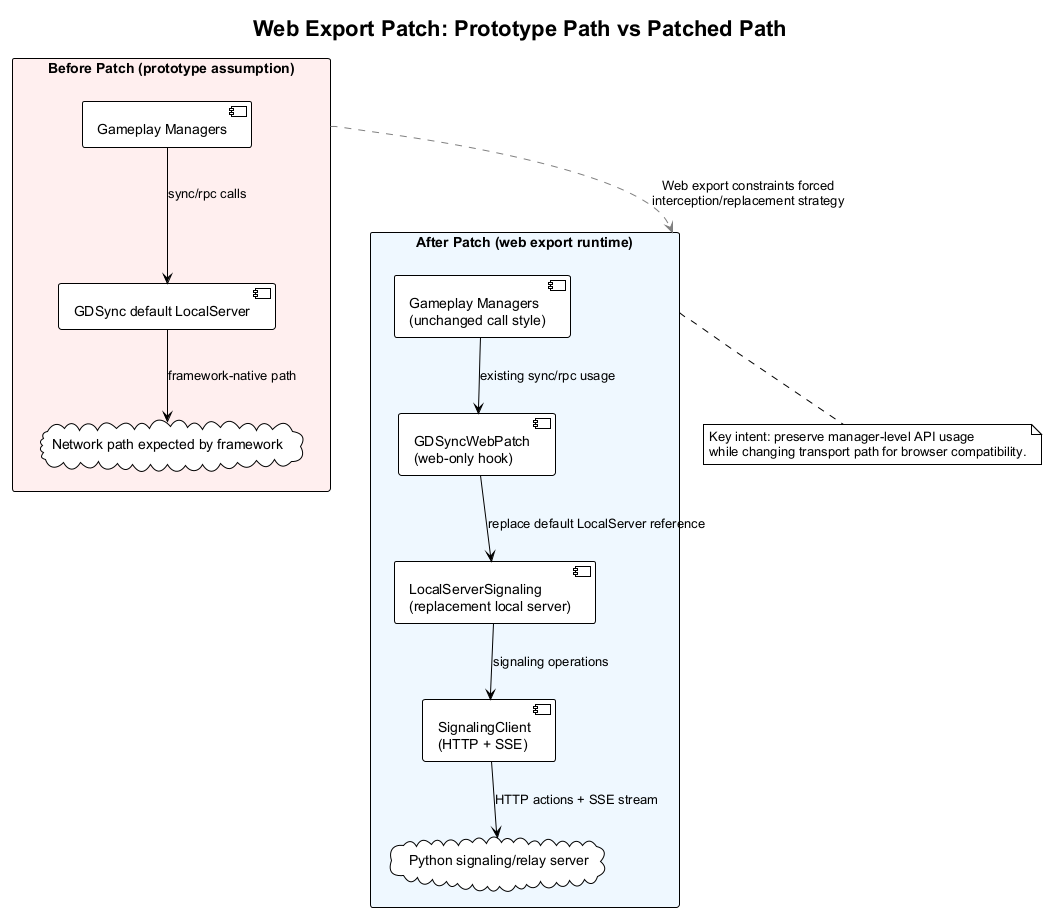
\includegraphics[width=0.95\textwidth]{figures/diagrams/web-patch-before-after}
    \caption{Prototype-to-web architecture diff showing LocalServer interception and relay-based replacement}
    \label{fig:web-patch-before-after}
\end{figure}

\begin{figure}[htbp]
    \centering
    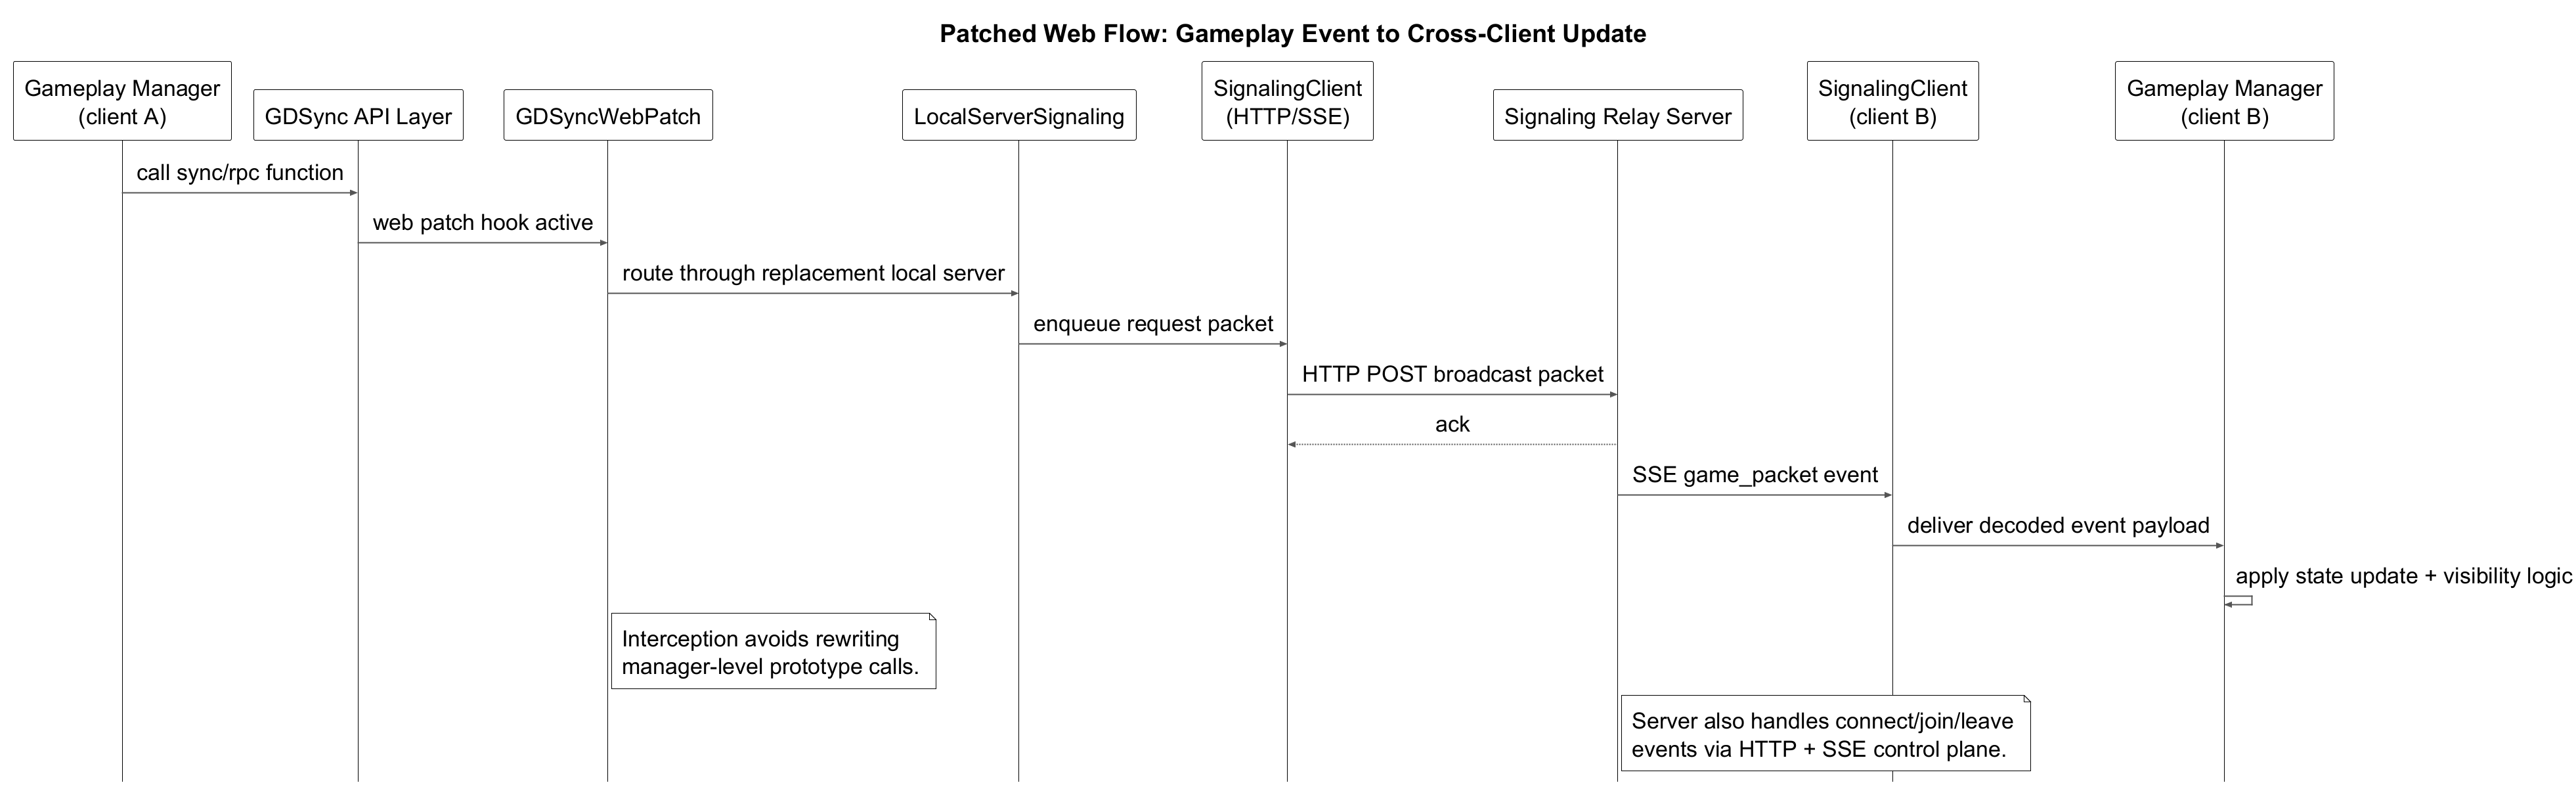
\includegraphics[width=0.95\textwidth]{figures/diagrams/web-patch-packet-event-sequence}
    \caption{Patched web signaling event sequence from gameplay call intent to synchronized client update}
    \label{fig:web-patch-packet-event-sequence}
\end{figure}

\begin{figure}[htbp]
    \centering
    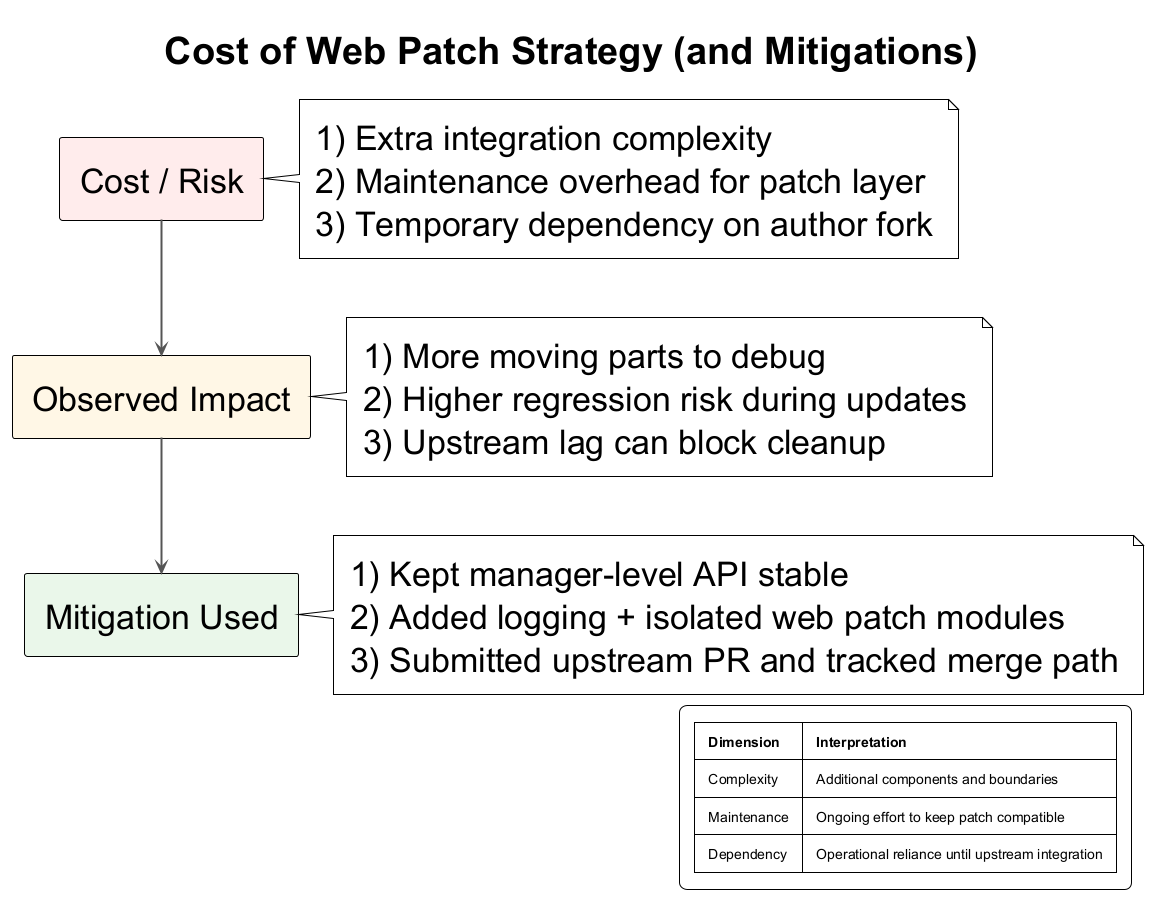
\includegraphics[width=0.9\textwidth]{figures/diagrams/web-patch-cost-summary}
    \caption{Cost of web-patch strategy: added complexity, maintenance burden, and temporary fork dependency}
    \label{fig:web-patch-cost-summary}
\end{figure}

The patch enabled continuity of the existing gameplay integration model but increased maintenance overhead, which is why a fork-plus-PR strategy was used as an interim operational path.

%-----------------------------------------------------------------------
\subsection{Debugging Multiplayer Issues}
\label{subsec:multiplayer-debugging}

\textbf{Challenge:}

Debugging multiplayer code is inherently difficult:
\begin{itemize}
    \item Requires multiple devices or instances
    \item Race conditions and timing-dependent bugs
    \item Network variability complicates reproduction
    \item Limited visibility into remote client state
\end{itemize}

\paragraph*{Solutions Implemented:}

\begin{enumerate}
    \item \textbf{Multi-Instance Testing}: Launched multiple Godot editor instances on the same machine
    \item \textbf{Network Logging}: Comprehensive logging of all network events with timestamps
    \item \textbf{State Dumps}: Ability to print full game state on command
    \item \textbf{Visual Indicators}: On-screen display of connection status, peer IDs, sync status
    \item \textbf{Replay System}: Recorded game events for post-mortem analysis
\end{enumerate}

%-----------------------------------------------------------------------
\section{Multiplayer Synchronization Challenges}
\label{sec:sync-challenges}

%-----------------------------------------------------------------------
\subsection{Card Order Synchronization}
\label{subsec:card-order-sync}

\textbf{Challenge:}

Maintaining consistent card ordering across clients proved more complex than anticipated. Issues included:
\begin{itemize}
    \item Godot's scene tree ordering not guaranteed to match logical ordering
    \item Child node order not automatically synchronized
    \item Timing differences causing transient inconsistencies
\end{itemize}

\textbf{Symptom:}

Cards appeared in different orders on different clients' screens, even though the underlying data was correct.

\textbf{Solution:}

\begin{enumerate}
    \item Implemented explicit position indices for cards
    \item Synchronized card order separately from card positions
    \item Used z-index to control visual stacking order
    \item Periodic consistency checks and resynchronization
\end{enumerate}

\begin{lstlisting}[caption={Card order synchronization approach}]
# Each card has an explicit order index
var card_order_index: int

# Synchronize order explicitly
@GDSync.rpc(call_local=true)
func sync_card_order(card_id: int, new_index: int):
    var card = get_card_by_id(card_id)
    card.card_order_index = new_index
    resort_cards_by_index()
\end{lstlisting}

%-----------------------------------------------------------------------
\subsection{Timing and Race Conditions}
\label{subsec:timing-issues}

\textbf{Challenge:}

Multiplayer systems are susceptible to race conditions:
\begin{itemize}
    \item Simultaneous card movements by different players
    \item Network messages arriving out of order
    \item Inconsistent state when players join mid-game
\end{itemize}

\textbf{Examples:}

\begin{itemize}
    \item Two players drag the same card simultaneously
    \item Player joins lobby after game has started
    \item Card deleted on host but still referenced on client
\end{itemize}

\textbf{Solutions:}

\begin{itemize}
    \item \textbf{Host Authority}: Only host can finalize state changes
    \item \textbf{Client Prediction with Rollback}: Show immediate feedback, then correct if host disagrees
    \item \textbf{State Snapshots}: New players receive full state snapshot on join
    \item \textbf{Defensive Programming}: Check object existence before operations
\end{itemize}

%-----------------------------------------------------------------------
\subsection{Different Client Views}
\label{subsec:client-views}

\textbf{Challenge:}

In multiplayer mode (OpenMP simulation), different players should see different cards in local buffers (simulating thread-private data), but maintaining this selective visibility while synchronizing the shared container was complex.

\paragraph*{Technical Issue:}

GDSync's node replication tries to keep all clients' scene trees identical, but selective visibility required different scene trees per client.

\textbf{Solution:}

\begin{itemize}
    \item Replicate all cards to all clients (for consistency)
    \item Use visibility flags to hide inappropriate cards
    \item Implement client-side filtering based on ownership metadata
    \item Synchronize ownership and visibility separately from positions
\end{itemize}

%-----------------------------------------------------------------------
\section{UI/UX Challenges}
\label{sec:mobile-ux-challenges}

%-----------------------------------------------------------------------
\subsection{Displaying Many Cards on Limited Screen Space}
\label{subsec:many-cards-small-screens}

\textbf{Challenge:}

Displaying 50--200 cards on screen (particularly on smaller browser viewports or touch-enabled devices) presents significant layout challenges:
\begin{itemize}
    \item Cards must be large enough to read and tap
    \item All cards must be accessible without excessive scrolling
    \item Layout must work in both portrait and landscape orientations
\end{itemize}

\paragraph*{Solutions Attempted:}

\begin{enumerate}
    \item \textbf{Grid Layout}: Cards arranged in a grid
          \begin{itemize}
              \item Pros: Space-efficient, familiar pattern
              \item Cons: Hard to see linear order, scrolling still required
          \end{itemize}

    \item \textbf{Scrollable Row (Selected Direction)}: Single row with horizontal scrolling
          \begin{itemize}
              \item Pros: Linear order visible, simple interaction
              \item Cons: Requires substantial scrolling with many cards
          \end{itemize}

    \item \textbf{Zoomable Canvas}: Pan and zoom to navigate cards
          \begin{itemize}
              \item Pros: Flexible navigation, can fit many cards
              \item Cons: Complex interaction, easy to get lost
          \end{itemize}

    \item \textbf{Hybrid Approach (Selected Direction)}:
          \begin{itemize}
              \item Grid layout with intelligent sizing
              \item Vertical scrolling for overflow
              \item Zoom controls for adjusting card size were explored but not fully implemented in the current version
          \end{itemize}
\end{enumerate}

%-----------------------------------------------------------------------
\subsection{Touch Interaction Precision}
\label{subsec:touch-precision}

\textbf{Challenge:}

Touch input is less precise than mouse input:
\begin{itemize}
    \item Finger occludes card being dragged
    \item Difficulty selecting specific cards when densely packed
    \item Accidental touches and swipes
\end{itemize}

\textbf{Solutions:}

\begin{itemize}
    \item \textbf{Offset Dragging}: Card rendered above finger with offset
    \item \textbf{Magnification}: Enlarge selected card for better visibility
    \item \textbf{Touch Feedback}: Visual and haptic feedback for touch events
    \item \textbf{Double-Tap Select}: Alternative to drag for card selection
    \item \textbf{Drop Zone Highlighting}: Clear indication of valid drop targets
\end{itemize}

%-----------------------------------------------------------------------
\subsection{Performance on Low-End Devices}
\label{subsec:lowend-performance}

\textbf{Challenge:}

Not all students have high-end hardware. The game needed to run acceptably across a range of devices and browsers, including low-end laptops and older browser versions.

\paragraph*{Performance Constraints:}

\begin{itemize}
    \item Limited GPU power for rendering many cards
    \item Lower memory (2--4 GB RAM)
    \item Slower network hardware
    \item Battery life concerns
\end{itemize}

\paragraph*{Optimization Strategies Considered:}

The following strategies were evaluated; not all were fully implemented in the current version:
\begin{itemize}
    \item Reduce draw calls through Godot's built-in 2D batching
    \item Viewport culling to avoid rendering off-screen cards (handled by Godot's built-in culling)
    \item Texture atlases to reduce texture swaps when rendering many card sprites
    \item Server-side gzip/Brotli compression of the exported WebAssembly and resource files, reducing the network transfer size from approximately 135~MB to 60~MB
\end{itemize}

Profiling showed that rendering bottlenecks were manageable for the target card counts (1--200), so more aggressive optimizations were not required (see Chapter~\ref{ch:results}, Section~\ref{subsec:export-size}).

%-----------------------------------------------------------------------
\section{Testing Challenges}
\label{sec:testing-challenges}

%-----------------------------------------------------------------------
\subsection{Multiplayer Testing Complexity}
\label{subsec:multiplayer-testing}

\textbf{Challenge:}

Testing multiplayer functionality requires:
\begin{itemize}
    \item Multiple devices or instances
    \item Coordination between test clients
    \item Reproduction of specific network conditions
    \item Testing edge cases (disconnections, late joins, etc.)
\end{itemize}

\paragraph*{Approaches:}

\begin{enumerate}
    \item \textbf{Multi-Instance Browser Testing}: Run multiple browser tabs or windows on development machine
    \item \textbf{Cross-Browser Testing}: Test on Chrome, Firefox, and Edge
    \item \textbf{Automated Test Scenarios}: Scripts to simulate player actions
    \item \textbf{Network Simulation}: Tools to introduce latency and packet loss
\end{enumerate}

\paragraph*{Limitations:}

\begin{itemize}
    \item Automated testing limited for interactive gameplay
    \item Difficult to reproduce exact timing of race conditions
    \item Real-world network conditions vary widely
\end{itemize}

%-----------------------------------------------------------------------
\subsection{Lack of Automated Testing}
\label{subsec:automated-testing}

\textbf{Challenge:}

Godot's testing ecosystem is less mature than traditional software development frameworks:
\begin{itemize}
    \item No built-in unit testing framework
    \item GUI testing particularly difficult
    \item Networking code hard to test in isolation
\end{itemize}

\paragraph*{Approach Taken:}

\begin{itemize}
    \item Manual testing with documented test cases
    \item Integration tests for critical paths
    \item Regression testing checklist before releases
    \item Community feedback as informal usability testing
\end{itemize}

\paragraph*{Future Improvement:}

\begin{itemize}
    \item Integrate GUT (Godot Unit Test) framework
    \item Develop automated test suite for core logic
    \item Implement continuous integration pipeline
\end{itemize}

%-----------------------------------------------------------------------
\section{Educational Design Challenges}
\label{sec:educational-challenges}

%-----------------------------------------------------------------------
\subsection{Balancing Accuracy and Playability}
\label{subsec:accuracy-vs-playability}

\textbf{Challenge:}

Educational games must balance pedagogical accuracy with engaging gameplay. Too much realism can reduce fun; too much simplification can create misconceptions.

\paragraph*{Trade-offs Made:}

\begin{itemize}
    \item \textbf{Simplified Memory Model}: Actual shared-memory systems have complex cache hierarchies not represented
    \item \textbf{Abstracted Synchronization}: Real OpenMP requires explicit barriers, locks, and atomic operations
    \item \textbf{Idealized Performance}: Network latency doesn't perfectly model memory access patterns
\end{itemize}

\textbf{Mitigation:}

\begin{itemize}
    \item Clear framing: "This is a metaphor, not a simulation"
    \item Post-game discussions to connect game to real concepts
    \item Accompanying documentation explaining simplifications
    \item Progressive difficulty introducing more complexity
\end{itemize}

%-----------------------------------------------------------------------
\subsection{Assessment of Learning Effectiveness}
\label{subsec:learning-assessment}

\textbf{Challenge:}

Demonstrating that the game actually improves learning outcomes requires formal educational research, including:
\begin{itemize}
    \item Pre/post-test measurements
    \item Control groups using traditional instruction
    \item Statistical analysis of results
    \item Long-term retention studies
\end{itemize}

\paragraph*{Limitations:}

Within the scope of this thesis, full educational efficacy studies were not feasible due to:
\begin{itemize}
    \item Time constraints
    \item Need for institutional review board approval
    \item Difficulty recruiting sufficient participants
    \item Complexity of isolating game's effect from other factors
\end{itemize}

\paragraph*{Future Work:}

Formal educational evaluation remains an important direction for future research, as discussed in Chapter~\ref{ch:conclusion}.

%-----------------------------------------------------------------------
\section{Lessons Learned}
\label{sec:lessons-learned}

%-----------------------------------------------------------------------
\subsection{Technical Lessons}
\label{subsec:technical-lessons}

\begin{enumerate}
    \item \textbf{Framework Evaluation}: Thoroughly evaluate third-party frameworks before committing; test advanced use cases early.

    \item \textbf{Abstraction Layers}: Isolate framework-specific code to facilitate future replacement if needed.

    \item \textbf{State Management}: Design clear state management patterns early; retrofitting is expensive.

    \item \textbf{Logging Infrastructure}: Comprehensive logging is essential for multiplayer debugging.

    \item \textbf{Performance Profiling}: Profile early and often; don't assume where bottlenecks are.
\end{enumerate}

%-----------------------------------------------------------------------
\subsection{Design Lessons}
\label{subsec:design-lessons}

\begin{enumerate}
    \item \textbf{User Testing}: Conduct user testing early; designer assumptions often wrong.

    \item \textbf{Responsive Design}: Design for varying viewport sizes and input methods from the start, not as an afterthought.

    \item \textbf{Simplicity}: Simpler interactions work better across input methods; complexity reduces usability.

    \item \textbf{Feedback}: Clear, immediate feedback is critical for learning and engagement.
\end{enumerate}

%-----------------------------------------------------------------------
\subsection{Process Lessons}
\label{subsec:process-lessons}

\begin{enumerate}
    \item \textbf{Iterative Development}: Iterative, incremental development surfaced issues early.

    \item \textbf{Version Control}: Frequent commits with clear messages saved time during debugging.

    \item \textbf{Documentation}: Documenting problems and solutions as they occurred proved invaluable.

    \item \textbf{Community Engagement}: Engaging with open-source communities provided solutions and support.
\end{enumerate}

%-----------------------------------------------------------------------
\section{Summary}
\label{sec:problems-summary}

This chapter documented the significant challenges encountered during development:

\begin{itemize}
    \item \textbf{Technology Challenges}: Engine trade-offs, framework limitations, and performance concerns
    \item \textbf{GDSync Issues}: Protected mode blocking, incomplete documentation, and debugging difficulty
    \item \textbf{Synchronization Complexity}: Card ordering, race conditions, and selective visibility
    \item \textbf{UI/UX}: Screen space constraints, touch/mouse interaction precision, and device performance variability
    \item \textbf{Testing Difficulty}: Multiplayer testing complexity and lack of automated testing tools
    \item \textbf{Educational Design}: Balancing accuracy with playability and assessing learning effectiveness
\end{itemize}

Importantly, this chapter also presented solutions and lessons learned that will benefit future developers of similar educational multiplayer games. The next chapter concludes the thesis and discusses future directions for research and development.


\input{chapters/08-conclusion}


%	BIBLIOGRAPHY
%-----------------------------------------------------------------------

\printbibliography[heading=bibintoc]


%	APPENDICES
%-----------------------------------------------------------------------

\appendix

\chapter{User Manual}
%-----------------------------------------------------------------------
% Appendix A: User Manual
%-----------------------------------------------------------------------

\section{Introduction}
\label{app:a:introduction}

This user manual provides instructions for accessing, configuring, and playing the HPC Sorting Serious Game. It is intended for students, educators, and anyone interested in learning about parallel computing through interactive gameplay.

The game is deployed as a \textbf{web application} (Godot Engine WebAssembly export) and runs directly in a modern browser. No installation is required for the primary deployment. Desktop (Windows) builds are also available for offline use or development.

%-----------------------------------------------------------------------
\section{System Requirements}
\label{app:a:system-requirements}

\subsection{Web Version (Primary)}

\begin{itemize}
    \item \textbf{Browser}: Chromium-based browser (Chrome, Edge, Brave) or Firefox, version 145 or later
    \item \textbf{WebGL}: WebGL 2.0 support required
    \item \textbf{JavaScript}: Must be enabled
    \item \textbf{RAM}: 2~GB minimum available to browser
    \item \textbf{Network}: Internet connection required for multiplayer mode; single-player works offline after initial load
    \item \textbf{Input}: Mouse or touchscreen
\end{itemize}

%-----------------------------------------------------------------------
\section{Accessing the Game}
\label{app:a:accessing}

\subsection{Web Version}

\begin{enumerate}
    \item Navigate to the hosted game URL in a supported browser
    \item Wait for the WebAssembly module to load (progress bar shown)
    \item The main menu appears once loading is complete
\end{enumerate}

\noindent\textbf{Note:} The web export is built with thread support disabled (\texttt{variant/thread\_support=false} in the Godot export preset), so COOP/COEP headers and \texttt{SharedArrayBuffer} are \emph{not} required. The game runs as a single-threaded WebAssembly application. Multiplayer communication uses HTTP/SSE, which does not depend on shared memory or cross-origin isolation.

%-----------------------------------------------------------------------
\section{Getting Started}
\label{app:a:getting-started}

\subsection{Main Menu}

On launch, the main menu presents the following options:
\begin{itemize}
    \item \textbf{Single Player}: Practice sorting alone (sequential execution baseline)
    \item \textbf{Multiplayer}: Join or host a cooperative multiplayer game (OpenMP shared-memory simulation)
    \item \textbf{Options}: Configure theme and display options
\end{itemize}

%-----------------------------------------------------------------------
\section{Single-Player Mode}
\label{app:a:singleplayer-mode}

\subsection{Starting a Single-Player Game}

\begin{enumerate}
    \item Select ``Single Player'' from the main menu
    \item Configure game parameters in the options dialog:
          \begin{itemize}
              \item \textbf{Number of cards}: configurable via spin box
              \item \textbf{Buffer slot count}: number of local buffer positions
              \item \textbf{Card value range}: upper bound for card values
          \end{itemize}
    \item Click ``Start'' to begin
\end{enumerate}

\subsection{Gameplay}

\paragraph*{Objective:}
Sort all cards in ascending order in the main container.

\paragraph*{Controls:}
\begin{itemize}
    \item \textbf{Drag and Drop}: Click and drag a card to reposition it within the container or move it to/from a buffer slot
    \item \textbf{Scroll}: Use the horizontal scroll bar or mouse wheel to navigate through cards when they exceed viewport width
\end{itemize}

\paragraph*{Using Buffer Slots:}
\begin{itemize}
    \item Buffer slots appear below the main card container
    \item Drag cards into buffer slots for temporary storage during sorting
    \item Buffer slots simulate thread-local storage in parallel computing
    \item Cards in buffers must form a contiguous subsequence of the sorted target before the game can complete
\end{itemize}

\paragraph*{Winning:}
\begin{itemize}
    \item The game completes when all cards are in correct ascending order in the main container
    \item Completion time is displayed
\end{itemize}

%-----------------------------------------------------------------------
\section{Multiplayer Mode}
\label{app:a:multiplayer-mode}

\subsection{Creating a Game}

\begin{enumerate}
    \item Select ``Multiplayer'' from the main menu
    \item Select ``Create Game''
    \item Configure game settings:
          \begin{itemize}
              \item Number of cards
              \item Buffer slot count per player
              \item Barrier mode (first-to-reach or round-robin)
          \end{itemize}
    \item A lobby code is generated automatically
    \item Share this code with other players
    \item Wait for players to join the lobby
    \item Once all players are present, click ``Start Game''
\end{enumerate}

\subsection{Joining a Game}

\begin{enumerate}
    \item Select ``Multiplayer'' from the main menu
    \item Select ``Join Game''
    \item Enter the lobby code provided by the host
    \item Click ``Join''
    \item Wait in the lobby for the host to start the game
\end{enumerate}

\subsection{Multiplayer Gameplay}

\paragraph*{Shared Container (Shared Memory):}
\begin{itemize}
    \item All cards are visible in the shared container, simulating shared memory accessible by all threads
    \item Any player can drag cards within the shared container to reorder them
    \item Changes propagate to all connected players in real time
\end{itemize}

\paragraph*{Local Buffers (Partitioned Shared Memory):}
\begin{itemize}
    \item Each player has local buffer slots visible only to themselves
    \item Cards moved to a player's buffer disappear from other players' views
    \item When a card is returned to the shared container, it becomes visible to all again
    \item This simulates the distinction between shared and private memory in OpenMP
\end{itemize}

\paragraph*{Barrier Synchronization:}
\begin{itemize}
    \item Any player can initiate a barrier (analogous to \texttt{\#pragma omp barrier})
    \item All players must reach the barrier before proceeding
    \item Once all players are at the barrier, a designated ``main thread'' (one player) can perform coordinated operations while others are blocked
    \item Main thread selection is either first-to-reach or round-robin, depending on game settings
    \item This teaches students about synchronization primitives in parallel computing
\end{itemize}

\paragraph*{Winning Together:}
\begin{itemize}
    \item The team wins when all cards are sorted correctly in the shared container
    \item All players must have returned their buffer cards to the container
\end{itemize}

%-----------------------------------------------------------------------
\section{Settings}
\label{app:a:settings}

\begin{itemize}
    \item \textbf{Theme}: Toggle between light and dark mode
    \item \textbf{Signaling Server URL}: Configure a custom signaling server address for multiplayer (advanced; defaults to the hosted server)
\end{itemize}

%-----------------------------------------------------------------------
\section{Tips and Strategies}
\label{app:a:tips-strategies}

\subsection{Sorting Strategies}

\begin{enumerate}
    \item \textbf{Divide and Conquer}: Use buffer slots to sort smaller subsets of cards, then merge them back
    \item \textbf{Find Sorted Runs}: Identify cards that are already in order and build around them
    \item \textbf{Minimize Moves}: Think before moving---unnecessary rearrangements waste time
\end{enumerate}

\subsection{Multiplayer Coordination}

\begin{enumerate}
    \item \textbf{Divide Responsibility}: Each player takes a value range (e.g., player~1 handles cards 1--25, player~2 handles 26--50)
    \item \textbf{Use Barriers Strategically}: Initiate a barrier when all players have sorted their portions and need to merge
    \item \textbf{Communicate Externally}: Use voice chat or messaging to coordinate since the game does not include built-in chat
    \item \textbf{Main Thread Awareness}: When you are the main thread during a barrier, merge sorted chunks efficiently; other players must wait
\end{enumerate}

%-----------------------------------------------------------------------
\section{Troubleshooting}
\label{app:a:troubleshooting}

\subsection{Common Issues and Solutions}

\paragraph*{Game does not load in browser:}
\begin{itemize}
    \item Verify that your browser supports WebGL 2.0 (check \texttt{chrome://gpu} in Chrome)
    \item Verify that JavaScript is enabled and WebGL 2.0 is supported (check \texttt{chrome://gpu} in Chrome)
    \item Try clearing browser cache and reloading
    \item Try a different Chromium-based browser
\end{itemize}

\paragraph*{Performance issues:}
\begin{itemize}
    \item Reduce the number of cards
    \item Close other browser tabs to free memory
    \item Ensure hardware acceleration is enabled in browser settings
\end{itemize}

\paragraph*{Cannot connect to multiplayer:}
\begin{itemize}
    \item Verify internet connection is active
    \item Check that both players are using the same game version
    \item Ensure the signaling server is reachable (default server requires internet access)
    \item Re-enter the lobby code carefully
    \item If using a custom signaling server, verify it is running and accessible
\end{itemize}

\paragraph*{Multiplayer desynchronization:}
\begin{itemize}
    \item This can occur if network packets are lost or arrive out of order
    \item The host can use the ``sync state'' mechanism to push authoritative state to all clients
    \item As a last resort, restart the game session
\end{itemize}

%-----------------------------------------------------------------------
\section{Educational Use}
\label{app:a:educational-use}

\subsection{For Students}

\begin{itemize}
    \item Play single-player mode first to understand the card sorting mechanics
    \item Observe how buffer slots help organize your sorting work (thread-local storage)
    \item In multiplayer, notice how coordination becomes harder with more players (communication overhead)
    \item Pay attention to the barrier mechanic---it directly mirrors \texttt{\#pragma omp barrier}
    \item Reflect on how game concepts relate to OpenMP parallel programming
\end{itemize}

\subsection{For Instructors}

\begin{itemize}
    \item Use as a pre-lecture activity to introduce HPC concepts before formal instruction
    \item The web deployment requires no installation---students can play immediately via a shared URL
    \item Facilitate post-gameplay discussion connecting game mechanics to parallel programming:
          \begin{itemize}
              \item Shared container $\leftrightarrow$ shared memory
              \item local buffers $\leftrightarrow$ thread-local / private variables
              \item Barrier mechanic $\leftrightarrow$ \texttt{\#pragma omp barrier}
              \item Multiple players $\leftrightarrow$ multiple threads
              \item Single-player $\leftrightarrow$ sequential execution baseline
          \end{itemize}
    \item Use completion metrics to discuss relative effort of parallel coordination vs.\ sequential sorting
\end{itemize}

%-----------------------------------------------------------------------
\section{Support and Resources}
\label{app:a:support}

\begin{itemize}
    \item \textbf{Game Repository}: \url{https://github.com/Siponek/hpc-sorting-serious-game}
    \item \textbf{Thesis Repository}: \url{https://github.com/Siponek/HPC-thesis}
    \item \textbf{Issue Tracker}: Report bugs and request features via GitHub Issues
    \item \textbf{License}: MIT license---contributions are welcome
\end{itemize}

%-----------------------------------------------------------------------


\chapter{Code Listings}
%-----------------------------------------------------------------------
% Appendix B: Code Reference
%-----------------------------------------------------------------------

\section{Source Code Repository}
\label{app:b:repository}

The complete source code for the HPC Sorting Serious Game is available as an open-source project:

\begin{itemize}
    \item \textbf{Game Repository}: \url{https://github.com/Siponek/hpc-sorting-serious-game}
    \item \textbf{GDSync Fork}: \url{https://github.com/Siponek/GD-Sync-fork} (web-export fix; upstream PR \#108)
    \item \textbf{License}: MIT License
    \item \textbf{Language}: GDScript (Godot Engine 4.x)
\end{itemize}

\section{Project Structure}
\label{app:b:structure}

The project follows Godot Engine conventions. The listing below shows the key directories and files relevant to this thesis:

\begin{verbatim}
hpc-sorting-serious-game/
+-- project.godot                 # Project configuration
+-- scene_manager.gd              # Global scene transition autoload
+-- settings.gd                   # Global settings autoload
+-- theme_manager.gd              # Dark/light theme autoload
+-- export_presets.cfg            # Export presets (Web, Windows, Android)
+-- scenes/
|   +-- CardScene/
|   |   +-- scripts/
|   |   |   +-- card_manager.gd  # Base card manager (705 lines)
|   |   +-- card_scene.tscn      # Card prefab scene
|   +-- MainMenuScene/
|   |   +-- menu_scene.tscn      # Main menu
|   |   +-- Singleplayer/
|   |   |   +-- singleplayer_options.gd
|   |   +-- Multiplayer/
|   |       +-- multiplayer_options.gd
|   +-- Singleplayer/
|   |   +-- singleplayer_scene.tscn
|   +-- Multiplayer/
|   |   +-- connection_manager.gd       # GDSync signal wiring (348 lines)
|   |   +-- MultiplayerGame/
|   |   |   +-- multiplayer_card_manager.gd  # Extends card_manager (1143 lines)
|   |   |   +-- barrier_manager.gd           # Barrier state machine (113 lines)
|   |   +-- Lobby/
|   |   |   +-- multiplayer_lobby.gd
|   |   +-- GDSyncWebPatch/
|   |       +-- gdsync_web_patch.gd          # Web platform patch (67 lines)
|   |       +-- local_server_signaling.gd    # HTTP-based LocalServer (~600 lines)
|   |       +-- signaling_client.gd          # HTTP/SSE signaling client
+-- addons/
|   +-- GD-Sync/                  # GDSync plugin (git submodule, forked)
|   +-- var_tree/                 # Runtime variable inspector
|   +-- toastparty/              # Toast notification plugin
|   +-- scene-selector/          # Scene selector plugin
+-- lib/
|   +-- logger/                  # Structured logging library
|   +-- feature_flag_handlers/   # Feature flag utilities
+-- res/
|   +-- algorithms/              # Algorithm description resources
|   +-- dark_theme.tres          # Dark theme resource
|   +-- menu_theme.tres          # Menu theme resource
|   +-- shaders/                 # Visual effect shaders
+-- signaling-server/
|   +-- server.py                # Python aiohttp signaling server
|   +-- server/                  # Server module package
|   +-- tests/                   # Server test suite
+-- exports/
|   +-- web-export/              # Web build output
|   +-- certs/                   # TLS certificates for local dev
\end{verbatim}

\section{Key Components}
\label{app:b:components}

\subsection{Card System}

\begin{itemize}
    \item \texttt{card\_manager.gd}: Base class handling card generation, drag-and-drop, buffer slot management, sorting validation (\texttt{check\_sorting\_order()}), buffer contiguity checking, and swap animations
    \item \texttt{multiplayer\_card\_manager.gd}: Extends \texttt{card\_manager.gd}; adds \texttt{CardState} serialization, GDSync function exposure, network broadcast/reconciliation, barrier integration, and visibility management for multi-player buffers
    \item \texttt{barrier\_manager.gd}: Three-state machine (\texttt{RUNNING} $\to$ \texttt{WAITING\_AT\_BARRIER} $\to$ \texttt{BARRIER\_ACTIVE}) implementing \texttt{\#pragma omp barrier} semantics with main-thread selection
\end{itemize}

\subsection{Networking and Multiplayer}

\begin{itemize}
    \item \texttt{connection\_manager.gd}: Autoload that wires GDSync signals (\texttt{connected}, \texttt{lobby\_created}, \texttt{client\_joined}, etc.) to game-level events; maintains typed player map
    \item \texttt{gdsync\_web\_patch.gd}: Autoload that detects \texttt{OS.has\_feature("web")} and replaces GDSync's native \texttt{LocalServer} with the HTTP/SSE-based \texttt{local\_server\_signaling.gd}
    \item \texttt{local\_server\_signaling.gd}: HTTP-based replacement for GDSync's \texttt{LocalServer}; preserves the original API contract while using the signaling server for packet relay
    \item \texttt{signaling\_client.gd}: HTTP/SSE client for lobby management and real-time event streaming
\end{itemize}

\subsection{Infrastructure}

\begin{itemize}
    \item \texttt{scene\_manager.gd}: Global autoload managing scene transitions with loading screen
    \item \texttt{settings.gd}: Global autoload storing game configuration (card count, buffer count, barrier mode, multiplayer flag)
    \item \texttt{theme\_manager.gd}: Dark/light theme switching
    \item \texttt{server.py}: Python signaling server built on \texttt{aiohttp}; handles lobby create/join, SSE event streaming, and game packet relay
\end{itemize}

\section{Configuration}
\label{app:b:configuration}

\subsection{Autoloads}

The following singletons are registered in \texttt{project.godot} and available globally:

\begin{itemize}
    \item \textbf{Settings}: Game parameters (card count, buffer count, barrier mode)
    \item \textbf{SceneManager}: Scene transitions
    \item \textbf{ThemeManager}: Visual theme control
    \item \textbf{ConnectionManager}: Multiplayer session state
    \item \textbf{GDSync}: Networking framework (third-party plugin)
    \item \textbf{GDSyncWebPatch}: Web-export compatibility layer
    \item \textbf{ToastParty}: User notification toasts
\end{itemize}

\subsection{Web Export Settings}

Key settings in the \texttt{export\_presets.cfg} Web preset:

\begin{itemize}
    \item \textbf{Export Format}: WebAssembly (WASM)
    \item \textbf{Thread Support}: Requires \texttt{SharedArrayBuffer} (COOP/COEP headers)
    \item \textbf{Canvas Resize Policy}: Responsive
    \item \textbf{Output}: \texttt{exports/web-export/} directory
\end{itemize}

\section{Building and Running}
\label{app:b:building}

\subsection{Development Setup}

\begin{enumerate}
    \item Install Godot Engine 4.x
    \item Clone the repository with submodules: \texttt{git clone --recursive}
    \item Open \texttt{project.godot} in the Godot Editor
    \item Press F5 to run locally (desktop mode)
\end{enumerate}

\subsection{Web Export}

\begin{enumerate}
    \item In Godot Editor: Project $\rightarrow$ Export
    \item Select the ``Web'' preset
    \item Click ``Export Project''
    \item Deploy the contents of \texttt{exports/web-export/} to a web server that sets the required COOP/COEP headers
\end{enumerate}

\noindent The project includes a \texttt{justfile} with automation targets for common tasks (formatting, linting, export, server management).

\subsection{Signaling Server}

The HTTP/SSE signaling server is in the \texttt{signaling-server/} directory:

\begin{enumerate}
    \item Install Python 3.10+ and dependencies: \texttt{pip install aiohttp aiohttp-cors}
    \item Run: \texttt{python server.py}
    \item Default port: 8765 (configurable)
\end{enumerate}

\noindent See Appendix~\ref{app:c} for the signaling server API reference.

%-----------------------------------------------------------------------


\chapter{API Documentation}
%-----------------------------------------------------------------------
% Appendix C: API Documentation
%-----------------------------------------------------------------------

\label{app:c}

\section{Introduction}
\label{app:c:introduction}

This appendix documents the APIs and interfaces of the HPC Sorting Serious Game, focusing on the signaling server REST/SSE endpoints and the key GDScript classes. The signaling server is the only custom server-side component; the game client is built in Godot Engine 4.x with GDScript.

%-----------------------------------------------------------------------
\section{Signaling Server API}
\label{app:c:signaling-server-api}

The signaling server is a Python application built on \texttt{aiohttp}. It serves three route groups: HTTP session management, HTTP lobby management with SSE, and WebSocket signaling for WebRTC.

\subsection{Session Endpoints}
\label{app:c:session-endpoints}

These endpoints manage rooms for WebRTC signaling.

\begin{table}[htbp]
    \centering
    \caption{Session management endpoints}
    \begin{tabular}{@{}llp{7cm}@{}}
        \toprule
        \textbf{Method} & \textbf{Path}                      & \textbf{Description}                                                                                                   \\
        \midrule
        \texttt{POST}   & \texttt{/session/host}             & Create a new room. Body: \texttt{\{channel, lobby\_name, public, player\_limit\}}. Returns \texttt{\{code, ws\_url\}}. \\
        \texttt{POST}   & \texttt{/session/join/\{code\}}    & Join a room by code or lobby name. Returns \texttt{\{code, ws\_url\}}.                                                 \\
        \texttt{POST}   & \texttt{/session/update/\{code\}}  & Update room metadata (lobby name, public flag, player limit).                                                          \\
        \texttt{POST}   & \texttt{/session/players/\{code\}} & Update player count for a room.                                                                                        \\
        \texttt{POST}   & \texttt{/session/close/\{code\}}   & Close a room and its associated lobby.                                                                                 \\
        \bottomrule
    \end{tabular}
\end{table}

\subsection{HTTP Lobby Endpoints (SSE)}
\label{app:c:lobby-endpoints}

These endpoints replace WebSocket-based lobby handling for browser compatibility. Real-time events are delivered via Server-Sent Events (SSE).

\begin{table}[htbp]
    \centering
    \caption{HTTP lobby endpoints}
    \begin{tabular}{@{}llp{7cm}@{}}
        \toprule
        \textbf{Method} & \textbf{Path}                  & \textbf{Description}                                                                                         \\
        \midrule
        \texttt{POST}   & \texttt{/api/lobby/connect}    & Connect and receive a peer ID. Optional body: \texttt{\{client\_id\}} to specify a GDSync client ID.         \\
        \texttt{POST}   & \texttt{/api/lobby/disconnect} & Disconnect from the server.                                                                                  \\
        \texttt{POST}   & \texttt{/api/lobby/create}     & Create a new lobby. Body: \texttt{\{lobby\_name, public, player\_limit\}}. Returns \texttt{\{code, lobby\}}. \\
        \texttt{POST}   & \texttt{/api/lobby/join}       & Join a lobby. Body: \texttt{\{code\}} or \texttt{\{lobby\_name\}}.                                           \\
        \texttt{POST}   & \texttt{/api/lobby/leave}      & Leave the current lobby.                                                                                     \\
        \texttt{GET}    & \texttt{/api/lobby/list}       & List public lobbies.                                                                                         \\
        \texttt{POST}   & \texttt{/api/lobby/broadcast}  & Broadcast a game packet to lobby peers. Body: \texttt{\{data\}}.                                             \\
        \texttt{GET}    & \texttt{/api/lobby/events}     & SSE event stream. Query: \texttt{?peer\_id=\{id\}}.                                                          \\
        \bottomrule
    \end{tabular}
\end{table}

\subsection{SSE Event Types}
\label{app:c:sse-events}

The SSE stream (\texttt{GET /api/lobby/events}) delivers the following event types:

\begin{table}[htbp]
    \centering
    \caption{SSE event types}
    \begin{tabular}{@{}lp{9cm}@{}}
        \toprule
        \textbf{Event}            & \textbf{Description}                            \\
        \midrule
        \texttt{welcome}          & Initial connection acknowledgement with peer ID \\
        \texttt{peer\_joined}     & A new peer joined the lobby                     \\
        \texttt{peer\_left}       & A peer left the lobby                           \\
        \texttt{lobby\_joined}    & Confirmation that this peer joined a lobby      \\
        \texttt{lobby\_closed}    & The lobby was closed (with reason)              \\
        \texttt{game\_packet}     & A game data packet relayed from another peer    \\
        \texttt{heartbeat}        & Keep-alive ping                                 \\
        \texttt{error}            & Error notification                              \\
        \texttt{server\_shutdown} & Server is shutting down                         \\
        \bottomrule
    \end{tabular}
\end{table}

\subsection{WebSocket Endpoints}
\label{app:c:websocket-endpoints}

These provide WebRTC signaling (for native desktop clients) and legacy WebSocket lobby handling:

\begin{table}[htbp]
    \centering
    \caption{WebSocket endpoints}
    \begin{tabular}{@{}lp{9cm}@{}}
        \toprule
        \textbf{Path}         & \textbf{Description}                                                                            \\
        \midrule
        \texttt{/ws/\{code\}} & WebRTC signaling channel. Exchanges ICE candidates, SDP offers/answers between peers in a room. \\
        \texttt{/lobby}       & WebSocket-based lobby management (native client usage; browser clients use HTTP+SSE instead).   \\
        \bottomrule
    \end{tabular}
\end{table}

\subsection{Utility Endpoints}
\label{app:c:utility-endpoints}

\begin{table}[htbp]
    \centering
    \caption{Utility endpoints}
    \begin{tabular}{@{}llp{7cm}@{}}
        \toprule
        \textbf{Method} & \textbf{Path}             & \textbf{Description}                                 \\
        \midrule
        \texttt{GET}    & \texttt{/health}          & Health check. Returns room, lobby, and peer counts.  \\
        \texttt{GET}    & \texttt{/rooms}           & List all active rooms.                               \\
        \texttt{GET}    & \texttt{/lobbies}         & List all lobbies with peer details.                  \\
        \texttt{GET}    & \texttt{/api/server/info} & Server information (version, uptime, configuration). \\
        \texttt{GET}    & \texttt{/}                & Welcome page / root info.                            \\
        \bottomrule
    \end{tabular}
\end{table}

\subsection{Error Codes}
\label{app:c:error-codes}

All error responses follow the format \texttt{\{"success": false, "error": "<code>", "message": "..."\}}.

\begin{table}[htbp]
    \centering
    \caption{Signaling server error codes}
    \begin{tabular}{@{}lp{9cm}@{}}
        \toprule
        \textbf{Code}               & \textbf{Meaning}                   \\
        \midrule
        \texttt{LOBBY\_NOT\_FOUND}  & Specified lobby does not exist     \\
        \texttt{LOBBY\_CLOSED}      & Lobby has been closed              \\
        \texttt{LOBBY\_FULL}        & Lobby has reached player limit     \\
        \texttt{ALREADY\_IN\_LOBBY} & Peer is already in a lobby         \\
        \texttt{NOT\_IN\_LOBBY}     & Peer is not in any lobby           \\
        \texttt{ROOM\_NOT\_FOUND}   & Specified room does not exist      \\
        \texttt{PEER\_NOT\_FOUND}   & Specified peer ID not found        \\
        \texttt{PEER\_ID\_IN\_USE}  & Requested peer ID is already taken \\
        \texttt{UNKNOWN\_COMMAND}   & Unrecognized message type          \\
        \texttt{INVALID\_JSON}      & Malformed JSON in request body     \\
        \bottomrule
    \end{tabular}
\end{table}

%-----------------------------------------------------------------------
\section{Server Data Models}
\label{app:c:server-models}

The signaling server uses two primary data models:

\paragraph{Peer:} Represents a connected player. Fields: \texttt{peer\_id} (int), \texttt{ws} (WebSocket connection, optional), \texttt{sse\_queue} (asyncio Queue for SSE events, optional), \texttt{player\_data} (dict), \texttt{lobby\_code} (str, optional). A peer uses either WebSocket \emph{or} SSE, not both---this dual-transport design enables both native and browser clients.

\paragraph{Lobby:} Represents a game lobby. Fields: \texttt{code} (str), \texttt{name} (str), \texttt{host\_id} (int), \texttt{public} (bool), \texttt{player\_limit} (int), \texttt{open} (bool), \texttt{created\_at} (ISO timestamp), \texttt{peers} (dict of Peer).

%-----------------------------------------------------------------------
\section{GDScript Game Classes}
\label{app:c:gdscript-classes}

This section summarizes the key GDScript classes. Full source code is available in the repository (see Appendix~\ref{app:b:repository}).

\subsection{CardManager (card\_manager.gd)}
\label{app:c:card-manager-class}

Base class managing all card logic for single-player mode.

\paragraph{Key Properties:}
\begin{itemize}
    \item \texttt{num\_cards: int} --- Number of cards in the game
    \item \texttt{cards\_array: Array} --- All card node instances
    \item \texttt{sorted\_all: Array} --- Sorted reference array (target ordering)
    \item \texttt{slots: Array} --- Buffer slot instances
    \item \texttt{card\_container: HBoxContainer} --- Shared card container (scene tree node)
\end{itemize}

\paragraph{Key Methods:}
\begin{itemize}
    \item \texttt{check\_sorting\_order() -> bool} --- Validates ascending order of cards in container
    \item \texttt{check\_player\_buffer\_contiguity() -> bool} --- Validates buffer cards form a contiguous sorted subsequence
    \item \texttt{generate\_completed\_card\_array(values, prefix) -> Array} --- Creates card instances from value array
    \item \texttt{create\_buffer\_slots() -> Array} --- Instantiates player buffer slots
    \item \texttt{animate\_card\_swap(card\_a, card\_b)} --- Animated card position swap with tween
\end{itemize}

\subsection{MultiplayerCardManager (multiplayer\_card\_manager.gd)}
\label{app:c:multiplayer-card-manager-class}

Extends \texttt{CardManager} for multiplayer mode.

\paragraph{Inner Class --- CardState:}
\begin{itemize}
    \item Serializable state object with \texttt{to\_dict()} and \texttt{from\_dict()} methods
    \item Fields: \texttt{value}, \texttt{index}, \texttt{original\_index}, \texttt{in\_container}, \texttt{in\_buffer}, \texttt{buffer\_owner}
\end{itemize}

\paragraph{Key Methods (GDSync-exposed):}
\begin{itemize}
    \item \texttt{sync\_complete\_game\_state(state\_data)} --- Full state reconciliation
    \item \texttt{sync\_card\_moved(value, from\_idx, to\_idx, client\_id)} --- Card repositioning
    \item \texttt{sync\_card\_entered\_buffer(value, player\_id)} --- Card enters public buffer
    \item \texttt{sync\_card\_left\_buffer(value, player\_id, new\_idx)} --- Card leaves buffer
    \item \texttt{barrier\_thread\_reached(player\_id)} --- Player reached barrier
    \item \texttt{barrier\_activate()} --- All threads at barrier; activate
    \item \texttt{barrier\_release()} --- Release barrier; resume normal play
\end{itemize}

\subsection{BarrierManager (barrier\_manager.gd)}
\label{app:c:barrier-manager-class}

Implements barrier synchronization state machine.

\paragraph{States:} \texttt{RUNNING} $\to$ \texttt{WAITING\_AT\_BARRIER} $\to$ \texttt{BARRIER\_ACTIVE} $\to$ \texttt{RUNNING}.

\paragraph{Key Methods:}
\begin{itemize}
    \item \texttt{enter\_waiting\_state(initiator\_id, all\_player\_ids)} --- Transition to waiting state
    \item \texttt{activate\_barrier()} --- Transition to active state (all threads arrived)
    \item \texttt{release\_barrier()} --- Reset and return to running state
    \item \texttt{determine\_main\_thread(first\_id, all\_ids) -> int} --- Select coordinator (first-to-reach or round-robin)
\end{itemize}

\paragraph{Signals:}
\begin{itemize}
    \item \texttt{barrier\_state\_changed(new\_state)} --- State transition notification
    \item \texttt{thread\_reached\_barrier(player\_id)} --- Player arrival notification
    \item \texttt{main\_thread\_assigned(player\_id)} --- Main thread selected
\end{itemize}

\subsection{ConnectionManager (connection\_manager.gd)}
\label{app:c:connection-manager-class}

Autoload that wraps GDSync signals into game-level events.

\paragraph{Key Methods:}
\begin{itemize}
    \item \texttt{am\_i\_host() -> bool} --- Whether local player is lobby host
    \item \texttt{get\_my\_client\_id() -> int} --- Local player's GDSync client ID
    \item \texttt{get\_player\_list() -> MultiplayerTypes.PlayersMap} --- Current player map
\end{itemize}

\paragraph{Key Signals:}
\begin{itemize}
    \item \texttt{player\_joined\_lobby(player\_id)} --- Player entered lobby
    \item \texttt{player\_list\_updated(players)} --- Player list changed
    \item \texttt{lobby\_joined(lobby\_name)} --- Local player joined a lobby
\end{itemize}

%-----------------------------------------------------------------------
\section{GDSync Framework Usage}
\label{app:c:gdsync-usage}

This project uses GDSync's explicit function exposure model. GDSync does \emph{not} use annotations or decorators for RPC. Instead, functions are registered at runtime:

\begin{lstlisting}[caption={GDSync function exposure (actual API)}]
# Expose a function for remote calls
GDSync.expose_func(self.my_function)

# Call function on all peers
GDSync.call_func(self.my_function, [arg1, arg2])

# Call function on a specific peer
GDSync.call_func_on(target_peer_id, self.my_function, [arg1, arg2])

# Expose a variable for synchronization
GDSync.expose_var(self, "variable_name")
\end{lstlisting}

\paragraph{Key GDSync Signals:}
\begin{itemize}
    \item \texttt{GDSync.connected} --- Successfully connected to server
    \item \texttt{GDSync.connection\_failed} --- Connection attempt failed
    \item \texttt{GDSync.lobby\_created} --- Lobby created (host)
    \item \texttt{GDSync.lobby\_joined} --- Joined an existing lobby
    \item \texttt{GDSync.client\_joined} --- A new client joined the lobby
    \item \texttt{GDSync.client\_left} --- A client left the lobby
    \item \texttt{GDSync.lobbies\_received} --- Lobby list received
\end{itemize}

\noindent For protected mode details and the web-export compatibility layer, see Chapter~\ref{ch:problems}, Section~\ref{subsec:protected-mode-issue} and Chapter~\ref{ch:implementation}, Section~\ref{sec:web-patch-implementation}.

%-----------------------------------------------------------------------


%TODO - add study materials (slides, exercises, etc.) as appendix D after the review
% \chapter{Study Materials}
% \input{appendices/appendix-d-study-materials}

%-----------------------------------------------------------------------

\end{document}
